\documentclass{ctexbook}

\usepackage{geometry}
\geometry{a4paper}
%\usepackage[UTF8, heading = false, scheme = plain]{ctex}%格式
\usepackage{ctex}
\usepackage{bm}
\usepackage{graphicx} %添加图片
\usepackage{amsthm}
\usepackage{amsmath}
\renewcommand{\vec}[1]{\boldsymbol{#1}} % 生产粗体向量,而不是带箭头的向量
\usepackage{amssymb}
\usepackage{booktabs} % excel导出的大表格
\usepackage{hyperref}
\usepackage{rotating}
\usepackage{extarrows}

%\newtheorem{definition}{Definition} %英文

%\newtheorem{theorem}{Theorem}

\newtheorem{definition}{定义}[section] %中文
\newtheorem{example}{例}[section]
\newtheorem{lemma}{引理}[section]

\newtheorem{theorem}{定理}[section]

%\newenvironment{proof}{{\noindent\it 证明}\quad}{\hfill □ \square□\par}

\DeclareMathOperator{\Ima}{Im}%定义新符号

\DeclareMathOperator{\Rank}{rank}%定义求秩算子

\title{\heiti 2022-2023 学年秋冬学期 \\ 线性代数I(H)期末复习讲义}
\author{2022-2023 秋冬线性代数 I(H)辅学期末复习授课 \\ 吴一航\ \ yhwu\_is@zju.edu.cn}

\begin{document}
\maketitle
\centerline{\huge \heiti 前言}
\vskip 0.3 in
\kaishu
线性代数作为一门重要的基础学科,是很多同学大一必修的课程,也是将来深入学习部分方向的基础。
竺院同学学习的《大学数学:代数与几何(第二版)》(居余马,李海中)授课的思路不同于国内绝大
部分的线性代数以及高等代数教材,从线性空间和线性映射出发引入矩阵,所以更加抽象,但是也
更加接近本质。

然而,这也导致可参考的资料有限。一般的线性代数以及高等代数教材都是从行列式入手,线性空间和
线性映射的内容要么在学完矩阵等内容后讲解,或者是根本不涉及。并且普通的考研数学也基本不涉及
这一部分,因此一直以来都只有《大学数学:代数与几何学习辅导》(林翠琴,居余马)一本教材的
配套辅导资料比较贴近,很多同学可能会参考国内的丘维声老师的高等代数或者是国外著名的MIT教授
Gilbert Strang 的网课,但内容还是略有差别,也比较耗费精力,对于很多同学而言并不是最好的
选择。虽然说学习知识更重要的在于体会其本质内容,体会其深入的思想,但现实问题
在于,缺少内容的总结以及题目的练习会使得很多同学无法适应这种抽象的学习思维。因此,我编写
本册的主要目的就在于给这一套教程一个合适的配套资料,使得同学们能在学习与复习时更加有头绪。

在编写与修订的过程中,我主要参考了教材《大学数学:代数与几何(第二版)》(居余马,李海中)
、《大学数学:代数与几何学习辅导》(林翠琴,居余马)、《高等代数(第二版)》(丘维声)、
《高等代数:学习指导书》(丘维声)、《线性代数辅导讲义》(汤家凤)、
《高等代数强化讲义》(李扬)以及《高等代数考研:高频真题分类精解300例》等,并参考了部分
历年试题。同时需要感谢谢集同学等在阅读过程中指出了本册中的一部分笔误。

在编写中,我主要按照2022-2023学年秋冬学期的考核要求编写,因此正交、正定等内容并未包含在内。
我的编写整体思路与教材章节顺序一致,除去高斯消元法的内容并未首先讲解,而是并入专题五中,如果
这一部分不够熟悉的同学,建议先阅读专题五的第一节内容。并且编写过程中我将教材及其辅导资料中
有价值的习题全部摘录,这些也是考试中很多习题的改编起点。除此之外,本册中多处内容提及教材中
相应内容,因此建议二者配套阅读。

除此之外,本册有一个精简版适用于期末短期复习,删除了部分较难的内容和习题,更加针对考试的难度,
如果对自己要求不是很高或者考前时间有限建议阅读精简版。

由于本人水平与时间有限,本册中可能还存在着一些问题,并且还有很多内容并没有详细展开提供严谨
的说明,答案的修订也比较仓促,希望各位见谅。如果条件允许,可以考虑开源共享源文件的方式,对
修订本册感兴趣的同学也可以参与进来,让本册更加完善,使得本册能更好地实现其目的。

最后,希望本册能对各位同学有所帮助,无论是对线性代数的学习与考试还是对未来遇见线性代数的
应用的情况。祝各位同学考试顺利,学有所成!

\begin{flushright}
    \songti 编者 \\
    2023年2月10日
\end{flushright}
\songti
\tableofcontents
\newpage
\setcounter{page}{1} % 将页码计数设置为1
\chapter{向量组与线性空间}

\section{Overview}
\begin{figure}[h]
	\centering
	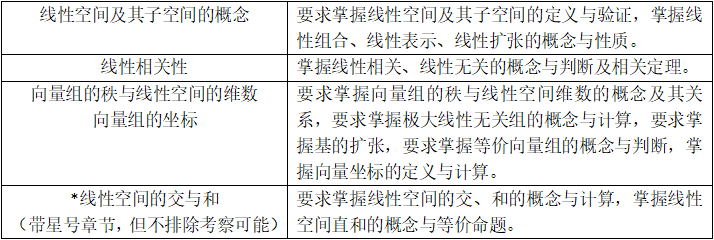
\includegraphics[scale=0.58]{1.png}
\end{figure}

\section{线性空间及其子空间的概念}
\subsection{线性空间的定义}
线性空间是我们接触的第一个比较重要的概念,它是定义在非空集合$V$和数域$\mathbf{F}$
上的,并且定义了$V$中的加法和$V\times \mathbf{F}$(即数域中的数与集合中向量之间的)数乘运算。
总结起来就是非空集合+数域+运算构成的。并且运算满足以下性质:

加法构成交换群$\langle V:+\rangle$(阿贝尔群,见教材1.10节,考试一般不要求)

1. 结合律:$a+(b+c)=(a+b)+c$;

2. 加法单位元:$\exists 0 \in V$,使得$\forall\alpha\in V$,有$a+0=0+a$;

3. 逆元:$\forall\alpha\in V,\exists b\in V$,有$a+b=b+a=0$,记$b=-a$;

4. 交换律:$\forall\alpha,\beta\in V, \alpha+\beta=\beta+\alpha$.

注意:加法零元和逆元是唯一的,我们可以定义减法运算为加上一个元素的逆。

数乘运算也满足四条性质:$\forall \alpha,\beta \in V,\forall \lambda,\mu\in\mathbf{F}$以及$\mathbf{F}$
上的乘法单位元1,有:

1. $1\cdot \alpha=\alpha$;

2. $\lambda(\mu\alpha)=(\lambda\mu)\alpha$;

3. $(\lambda+\mu)\alpha=\lambda\alpha+\mu\alpha$;

4. $\lambda(\alpha+\beta)=\lambda\alpha+\lambda\beta$.

注意,综合上述性质我们有方程$\lambda\beta+\lambda_1\alpha_1+\lambda_2\alpha_2+\cdots+\lambda_r\alpha_r=0$
在$\lambda\neq 0$时的解为$\beta=-\lambda^{-1}\lambda_1\alpha_1+-\lambda^{-1}\lambda_2\alpha_2+\cdots+-\lambda^{-1}\lambda_r\alpha_r$.

以上定义请务必牢记于心,考试可能要求你验证线性空间。记忆难度也并不大,阿贝尔群四条性质都有名称标注,
数乘运算也是结合律和分配律加单位元。

注意线性空间还有一个重要的概念是运算封闭,即线性空间中的元素进行加法或数乘运算后,得到的元素仍然是属于线性空间的。
这一点是定义要求的,加法封闭是阿贝尔群的要求,数乘请参考教材定义的要求。
\subsection{线性空间举例}
我们介绍三个常见的线性空间:

1. (多项式)$\mathbf{F}[x]_{n+1}=\{a_0+a_1x+\cdots+a_nx^n\ |\ a_i\in\mathbf{F}\}$构成线性空间,但
$$\mathbf{F}[x]_{n+1}=\{a_0+a_1x+\cdots+a_nx^n\ |\ a_i\in\mathbf{F},a_i\neq 0\}$$
不构成线性空间。

注:书上常将多项式记为$\mathbf{F}[x]_{n+1}$,表示次数不超过$n$的多项式的集合。

常见记号:$(k_1p_1+k_2p_2)(x)=k_1p_x(x)+k_2p_2(x)$。

2. (复数与实数)可以验证:全体复数构成的集合是数域$\mathbf{C}/\mathbf{R}$上的线性空间。此处一定注意复数$\mathbf{C}$在此处同时出现在集合和数域中。

注意:这一例子表明,同一集合可以在不同数域上构成不同的线性空间。特别是可以验证,线性空间$\mathbf{C(C)}$维数为1,不同于线性空间$\mathbf{C(R)}$维数为2。

当然,不同的集合也可以在同一个数域上构成不同的线性空间,例如$\mathbf{C(R)}$和$\mathbf{R(R)}$。

3. (线性方程组的解)可以验证,齐次线性方程组$AX=0$的解集是线性空间$\mathbf{F^n}$的一个子空间,但非齐次线性方程组的解不再构成线性空间,因为加法运算不封闭。(具体见教材P62的2.2节开头的例子以及P86习题3(3))。
\subsection{线性子空间}
我们首先看线性子空间的定义:
\begin{definition}
	设$W$是线性空间$V(\mathbf{F})$的非空子集,如果$W$对$V$中的运算也构成域$\mathbf{F}$
	上的线性空间,则称$W$是$V$的线性子空间(简称子空间).
\end{definition}
请一定注意定义中的非空子集,建议验证子空间时先验证非空。接下来是验证子空间的一般方法:
\begin{theorem}
	线性空间$V(\mathbf{F})$的非空子集$W$为$V$的子空间的充分必要条件是$W$对于$V(\mathbf{F})$的线性运算封闭.
\end{theorem}
这表明只要子空间中的元素满足对原空间的加法和数乘运算封闭即可。

注意线性空间有两个子空间称为平凡子空间,即仅含零元的子集$\{0\}$和其自身$V$。其它
子空间称为非平凡子空间。
\begin{example}
	\textup{(1)}说明$\mathbf{R}[x]_2$是$\mathbf{R}[x]_3$的子空间\textup{;}

	\textup{(2)}判断$W_1=\{(x,y,z)\ |\ \cfrac{x}{3}=\cfrac{y}{2}=z\},
	W_2=\{(x,,y,z)\ |\ x+y+z=1,x-y+z=1\}$是否为$\mathbf{R}^3$的子空间.
\end{example}
第二小问表明过原点的直线/平面构成三维空间的子空间,不过原点的无法保持线性性。

接下来我们讨论线性扩张及其性质,我们首先来看线性组合和线性表示的概念:
\begin{definition}
	设$V(\mathbf{F})$是一个线性空间,$\alpha_i\in V,\lambda_i\in \mathbf{F}(i=1,2,\cdots,m)$,
	则向量$\alpha=\lambda_1\alpha_1+\lambda_2\alpha_2+\cdots+\lambda_m\alpha_m$
	称为向量组$\{\alpha_1,\alpha_2,\cdots,\alpha_m\}$在域$\mathbf{F}$的线性组合,或说$\alpha$
	在域$\mathbf{F}$上可用向量组$\{\alpha_1,\alpha_2,\cdots,\alpha_m\}$线性表示.
\end{definition}
基于此,我们给出线性扩张的定义:
\begin{definition}
	设$S$是线性空间$V(\mathbf{F})$的非空子集,我们称
	$$L(S)=\{\lambda_1\alpha_1+\cdots+\lambda_k\alpha_k\ |\ \lambda_1,\cdots,\lambda_k\in\mathbf{F},\alpha_1,\cdots,\alpha_k\in S,k\in\mathbf{N^*}\}$$
	为$S$的线性扩张,即$S$中所有有限子集在域$\mathbf{F}$上的一切线性组合组成的$V(\mathbf{F})$的子集.
\end{definition}
下面的定理告诉我们可以通过线性扩张构造子空间:
\begin{theorem}
	线性空间$V(\mathbf{F})$的非空子集$S$的线性扩张$L(S)$是$V$中包含$S$的最小子空间.
\end{theorem}
这一定理的证明首先证明线性扩张是子空间,这是容易的,然后说明最小只需要说明$L(S)$是$V$中包含$S$的任意子空间的子集即可。

最后我们再说明有限维线性空间和无限维线性空间的定义,本课程研究的内容都在有限维线性空间:
\begin{definition}
	$V(\mathbf{F})$称为有限维线性空间,如果$V$中存在一个有限子集$S$使得$L(S)=V$,反之称为无限维线性空间.
\end{definition}
\begin{example}
	证明:$\mathbf{R}[x]_3$是有限维线性空间,$\mathbf{R}[x]$是无限维线性空间.
\end{example}
\subsection{习题}
\centerline{\heiti A组}
\begin{enumerate}
	\item 检验下列集合对指定的加法和数乘运算是否构成实数域上的线性空间.
	
	(1)有理数集$\mathbf{Q}$对普通的数的加法和乘法;

	(2)集合$\mathbf{R}^2$对通常的向量加法和如下定义的数量乘法:$\lambda\cdot(x,y)=(\lambda x,y)$;

	(3)$\mathbf{R}_+^n$(即$n$元正实数向量)对如下定义的加法和数乘运算:
	$$(a_1,\cdots,a_n)+(b_1,\cdots,b_n)=(a_1b_1,\cdots,a_nb_n),$$
	$$\lambda\cdot(a_1,\cdots,a_n)=(a_1^\lambda,\cdots,a_n^\lambda).$$

	(4)请继续完成教材P86第二章习题第一题9-11小问关于函数的加法数乘定义线性空间的问题.
	\item 请完成教材P86-86第二章习题第三题的全部小问.第5小问平常问题较多,实际上就是要判断满足一定条件的
	多项式是否构成子空间.
\end{enumerate}
\centerline{\heiti B组}
\begin{enumerate}
	\item 设$V$是一个线性空间,$W$是$V$的子集,证明:$W$是$V$的子空间$\iff L(W)=W$.
	\item 回答以下两个问题:

	(1)设$\mathbf{R}^+$是所有正实数组成的集合,加法和数乘定义如下:$\forall a,b \in \mathbf{R}^+,k\in \mathbf{R},a\oplus b = ab, k\odot a = a^k$,$\mathbf{R}^+$关于这一加法和数乘构成一个实线性空间,求$\mathbf{R}^+$的一组基;

	(2)设$V$是一个$n$维实线性空间,证明:存在$V$中的一个由可列无穷多个向量组成的向量组$\{\alpha_i\ |\ i\in\mathbf{Z}^+\}$,使得其中任意$n$个向量组成的向量组都是$V$的一组基.
\end{enumerate}
\centerline{\heiti C组}
\begin{enumerate}
	\item 设$E$是域$F$的一个子域.
	
	(1)证明:$F$关于自身的加法和乘法构成一个$E$上的向量空间,并举一例;

	(2)举例说明:$E(E\neq F)$不是$F$上的线性空间;

	(3)证明:若$V$是$F$上的一个线性空间,则$V$也是$E$上的一个线性空间.
\end{enumerate}

\section{线性相关性}
\subsection{线性相关性的定义}
研究线性相关性来源于我们希望知道有限维线性空间至少需要多少个向量张成,以下是其定义:
\begin{definition}
	设$V(\mathbf{F})$是一个线性空间,$\alpha_1,\alpha_2,\cdots,\alpha_m\in V$,如果存在
	不全为$0$的$\lambda_1,\lambda_2,\cdots,\lambda_m\in\mathbf{F}$,使得
	$$\lambda_1\alpha_1+\alpha_2\lambda_2+\cdots+\lambda_m\alpha_m=0$$
	成立,则称$\alpha_1,\alpha_2,\cdots,\alpha_m$线性相关,否则称线性无关(即系数只能为$0$).
\end{definition}
线性相关和线性无关的证明就是基于这个定义,请务必牢牢掌握。

直接由定义我们可以导出以下结论:

1. 线性空间中单个向量$\alpha$线性相关的充要条件是$\alpha$为零向量;

2. 任何含零向量的向量组都线性相关.

我们来看几个基本的例子:
\begin{example}
	\textup{(1)}判断$(1,1,0),(0,1,1),(1,0,-1)$的线性相关性;

	\textup{(2)}判断$(1,-3,1),(-1,2,-2),(1,1,3)$的线性相关性;

	\textup{(3)}判断$p_1(x)=1+x,p_2(x)=1-x,p_3(x)=x+x^2$的线性相关性;

	\textup{(4)}判断$1,\sin^2x,\cos^2x$的线性相关性;

	\textup{(5)}判断$1,2^x,2^{-x}$的线性相关性.
\end{example}
注意上述3-5题为不能代入特殊的$x$值来说明,例如(3)令$x=0$得到线性相关的做法是错误的,因为
(3)中线性空间就是多项式构成的线性空间,其中的元素就是多项式,不能代入值。注意(5)是特殊题型,
需要构造更多的方程来求解这一问题。
\subsection{线性相关性的定理}
本节内容十分重要,是理解线性空间结构的基础,希望同学们对以下定理及其证明十分熟练并且要有深刻的理解。
我们的主线思路是从不同方面理解线性相关性:
\begin{enumerate}
	\item 从线性组合看(定义)
	
	向量组线性相关$\iff$它们有系数不全为0的线性组合等于零向量;
	
	向量组线性无关$\iff$它们只有系数全为0的线性组合才会等于零向量。
	\item 从线性表示看(教材定理2.3)
	\begin{theorem}
		线性空间$V(\mathbf{F})$中的向量组$\alpha_1,\alpha_2,\cdots,\alpha_m(m \ge 2)$线性相关的充分必要条件是
		$\alpha_1,\alpha_2,\cdots,\alpha_m$中有一个向量可由其余向量在域$\mathbf{F}$上线性表示.
	\end{theorem}
	这一定理等价描述为,向量组线性无关的充分必要条件是其中的向量无法互相表示。这是显然的,因为向量组能互相表示
	利用定义可以轻松写出非零系数的线性表示。总结一下即为:

	向量组线性相关$\iff$其中至少有一个向量可以由其余向量线性表示;
	
	向量组线性无关$\iff$其中每一个向量都不能由其余向量线性表出。
	\item 从齐次线性方程组看(教材P66例3,实际上这一点与定义十分类似)

	列向量组$\alpha_1,\alpha_2,\cdots,\alpha_m$线性相关$\iff$齐次线性方程组$x_1\alpha_1+x_2\alpha_2+\cdots+x_m\alpha_m=0$有非零解;

	列向量组$\alpha_1,\alpha_2,\cdots,\alpha_m$线性无关$\iff$齐次线性方程组$x_1\alpha_1+x_2\alpha_2+\cdots+x_m\alpha_m=0$只有零解。
	\item 从向量组线性表示一个向量的方式看(教材定理2.4)
	\begin{theorem}
		若向量组$\alpha_1,\alpha_2,\cdots,\alpha_m$线性无关,而向量组$\beta,\alpha_1,\alpha_2,\cdots,\alpha_m$线性相关,
		则$\beta$可由$\alpha_1,\alpha_2,\cdots,\alpha_m$线性表示,且表示法唯一.
	\end{theorem}
	总结如下:若向量组外另一向量可由这一组向量线性表示,则

	向量组线性无关$\iff$表出方式唯一;

	向量组线性相关$\iff$表示方式有无穷多种。

	表示方式唯一的证明是经典的,即设有另一种表示方式,然后利用线性无关的定义说明这两种表示方式必定相同即可。
	\item 从向量组与它的部分组的关系看(教材P67例6)
	
	如果向量组的一个部分组线性相关,那么整个向量组也线性相关;

	如果向量组线性无关,那么它的任何一个部分组也线性无关。
\end{enumerate}
除此之外,我们还可以从矩阵的秩以及行列式是否为0的角度理解,这些内容后续会有介绍。

最后我们还要介绍一个定理,这一定理更加重要,证明可能较为复杂,但结论一定要熟练掌握:
\begin{theorem}
	设$V(\mathbf{F})$中向量组$\{\beta_1,\beta_2,\cdots,\beta_s\}$的每个向量可由另一向量组$\alpha_1,\alpha_2,\cdots,\alpha_r$
	线性表示.若$s>r$,则$\{\beta_1,\beta_2,\cdots,\beta_s\}$线性相关.
\end{theorem}
这一定理的等价命题为,$\{\beta_1,\beta_2,\cdots,\beta_s\}$线性无关则必有$s\le r$。

这一定理可通俗概括为:多的向量组可以被少的向量组线性表示,多的一定线性相关。反过来说,线性无关的向量只能被等长或更长的向量组线性表示。
\subsection{习题}
\centerline{\heiti A组}
\begin{enumerate}
	\item 请先完成教材P87-88第二章习题第10题的判断题;
	\item 证明:如果向量组线性相关,把每个向量去掉$m$个位置一致的分量,得到的缩短组仍线性相关;
	如果向量组线性无关,把每个向量添加$m$个位置一致的分量,得到的缩短组仍线性无关;
	\item $a$取何值时,$\beta_1=(1,3,6,2)^\mathrm{T},\beta_2=(2,1,2,-1)^\mathrm{T},\beta_3=(1,-1,a,-2)^\mathrm{T}$
	线性无关?
	\item 设$\alpha_1,\alpha_2,\cdots,\alpha_n\in\mathbf{F}^n$,证明:$\alpha_1,\alpha_2,\cdots,\alpha_n$线性无关
	的充要条件是$\mathbf{F}^n$中任一向量都可以由它们线性表示.
	\item 设$S_1=\{\alpha_1,\cdots,\alpha_s\},S_2=\{\beta_1,\cdots,\beta_t\}$是向量空间$V$的两个线性无关的子集,证明:
	$\alpha_1,\cdots,\alpha_s,\beta_1,\cdots,\beta_t$线性无关$\iff L(S_1)\cap L(S_2)=\{0\}$.
\end{enumerate}
\centerline{\heiti B组}
\begin{enumerate}
	\item 已知$\alpha_1\neq 0$,则$\alpha_1,\alpha_2,\cdots,\alpha_n$线性相关的充要条件是存在$i(2\le i\le n)$
	使得$\alpha_i$可由$\alpha_1,\alpha_2,\cdots,\alpha_{i-1}$线性表示,且表示法唯一.
	\item 设 $\sigma$ 是线性空间 $V$ 上的线性变换,如果 $\sigma^{k-1}(\alpha) \neq 0$,但 $\sigma^{k}(\alpha) = 0$,证明:\newline
	$\alpha,\ \sigma(\alpha),\ \dots,\ \sigma^{k-1}(\alpha)(k>0)$ 线性无关
	(本题还有对应的矩阵版本,解法基本一致).

	注:以上两题要采用从右向左/从左向右检查第一个不为0的系数的方法,这种思想是重要的.
	\item 设向量组$\alpha_1,\alpha_2,\cdots,\alpha_n$线性无关,在向量组$\beta,\alpha_1,\alpha_2,\cdots,\alpha_n$中至多有一个向量$\alpha_i(1\le i\le r)$
	可被其前面的$i$个向量$\beta,\alpha_1,\alpha_2,\cdots,\alpha_{i-1}$线性表示.
	\item 证明:$1,e^{\lambda_1\cdot x},e^{\lambda_2\cdot  x}(\lambda_1\neq\lambda_2$且均不为0$)$线性无关.
\end{enumerate}
\centerline{\heiti C组}
\begin{enumerate}
	\item 如果$n$阶方阵$A_1,A_2,\cdots,A_m$满足$A_i^2\neq O(i=1,2,\cdots,m)$,且当$i\neq j$时,$A_iA_j=O$,
	证明:$m\le n$.
	\item 已知$m$个向量$\alpha_1,\alpha_2,\cdots,\alpha_m$线性相关,但其中任意$m-1$个都线性无关,证明:
	
	(1)若$k_1\alpha_1+\cdots+k_m\alpha_m=0$,则$k_1,\cdots,k_m$全为0或全不为0;

	(2)若存在两个等式
	$$k_1\alpha_1+\cdots+k_m\alpha_m=0,$$
	$$l_1\alpha_1+\cdots+l_m\alpha_m=0,$$
	其中$l_1\neq 0$,证明:$\cfrac{k_1}{l_1}=\cdots=\cfrac{k_m}{l_m}$.
\end{enumerate}

\section{向量组的秩\ 线性空间的维数\ 向量组的坐标}
\subsection{秩与维数的概念}
\begin{definition}
	若线性空间$V(\mathbf{F})$的非空子集$S$中存在线性无关的向量组$B=\{\alpha_1,\alpha_2,\cdots,\alpha_m\}$,
	且$S$中每个向量都可以由$B$线性表示,则$B$中向量的个数$r$叫做$S$的秩,记作$r(S)= r$(实际上即为极大线性无关组的长度).
\end{definition}
\begin{definition}
	若线性空间$V(\mathbf{F})$的有限子集$B=\{\alpha_1,\alpha_2,\cdots,\alpha_n\}$线性无关,且$L(B) = V$,则称$B$为$V$的一组基,
	并称$n$为$V$的维数,记作$\dim V = n$.
\end{definition}
实际上,综合上述两个定义我们可以看到,如果$S$为有限维线性空间$V(\mathbf{F})$的子空间,那么$S$的秩就是$S$的维数。

从维数的定义中我们可以理解到,一个线性空间的基的长度必定是唯一的,否则同一个线性空间将会出现多个不同的维数,这是不合理的。
证明可以直接利用上一小节中的定理1.3.3,反证法即可。当然我们也可以不利用定理1.3.3,直接通过线性无关的定义以及线性方程组的解的情况讨论
得到线性空间维数唯一的结论(大家可以自行尝试,实际上我的期中复习2021版中也有讲解)。

我们需要提及一个概念,即自然基。例如三维空间的自然基为$(1,0,0),(0,1,0),(0,0,1)$,$n$维空间也有类似的推广(即$n$个只有一位为0其余全为1的向量)。
对于多项式我们则将$1,x,x^2,\cdots$称为自然基,矩阵、函数等也有相关的常用的基。
\subsection{相关定理与性质}
根据秩与维数的概念与定理1.3.3(或教材定理2.5),我们可以得到以下直接的结论:

1. $r(S)=n$,则$S$中$n+1$个向量必线性相关,$S$中任何线性无关向量组至多含$n$个向量,且将含$n$个线性无关向量的
向量组称为$S$的极大线性无关组。同理,$n$维线性空间中$n+1$个向量必线性相关,其中含$n$个线性无关向量的向量组称为
线性空间的一组基;

注意:极大线性无关组有两个关键词:线性无关与张成空间,我们还有两个结论:
\begin{itemize}
	\item 设向量组的秩为$r$,则它的任意$r$个线性无关的向量都构成它的一个极大线性无关组;
	\item 设向量组的秩为$r$,则若向量组可以由其中的$r$个向量线性表出,那么这$r$个向量就是原向量组的一个极大线性无关组。
\end{itemize}

2. 线性空间的基的个数(维数)是唯一的,但基中向量选取不唯一;

3. 若$r(S)=r$,$B=\{\alpha_1,\alpha_2,\cdots,\alpha_r\}$是$S$的极大线性无关组,则$L(S)=L(B)$,
即$\dim L(S)=r(S)$(秩与维数统一).

接下来我们介绍等价向量组的概念。我们称可以互相线性表示的两个向量组为等价向量组。可以回忆教材1.3节等价关系,可知等价向量组必须满足自反性、对称性以及传递性。
这一点是容易证明的。注意,等价向量组必定秩相等,这是由定理1.3.3(教材定理2.5)可以直接导出的。
关于等价向量组,在后续专题过渡矩阵中还有更多的讨论。

实际上上述结论将向量组的线性扩张替换为线性空间,向量组的秩替换为线性空间的维数,向量组的极大线性无关组替换为线性空间的基,
我们能得到大量等价的结论。除此之外还有和线性相关性以及秩有关的很多结论,我们在这两节习题中展示。
\begin{example}
	证明以下两个结论:

	\textup{(1)}设$U$和$W$都是$V$的非零子空间,如果$U\subseteq W$,那么$\dim U \le \dim W$;
	
	\textup{(2)}设$U$和$W$都是$V$的非零子空间,$U\subseteq W$,且$\dim U = \dim W$,则$U = W$.
\end{example}
最后是一个很重要的定理,这一定理在之后大量的定理证明中都有运用:
\begin{theorem}
	如果$W$是$n$维线性空间$V$的一个子空间,则$W$的基可以扩充为$V$的基.
\end{theorem}
这一定理表明我们可以往一个向量组添加向量扩充为基,之前我们通过求极大线性无关组丢掉一些向量
使得我们获得一组基。定理证明是简单的,实际上这就是教材定理2.6。
\subsection{求解极大线性无关组}
我们首先考察一个阶梯矩阵$A$。我们不难发现,阶梯矩阵的主元(非零行的第一个非零元素)所在的列
构成$A$的列向量的一个极大线性无关组。证明可以利用行列式的秩的相关概念,取出矩阵的子式考虑其行列式。

但我们一般的题目不会直接给出能够成阶梯矩阵的向量,但我们知道,矩阵经过初等行变换不改变列之间的
线性关系(思考其证明),所以我们求极大线性无关组的方法就是,将向量按列排列成矩阵,然后对矩阵做
初等行变换,化为阶梯形,找到主元所在的列,对应的原向量即组成一个极大线性无关组。

注意极大线性无关组是不唯一的,但上面给出了一个程式化的方法。实际上如果能一眼看出结果的也不必如此麻烦
(当然题目直接要求极大线性无关组还是应当写具体过程的)。
\begin{example}
	求向量组$\{\alpha_1=(1,-1,2,4),\alpha_2=(0,3,1,2),\alpha_3=(3,0,7,14),\alpha_4=(1,-1,2,0),\alpha_5=(2,1,5,6)\}$
	的极大线性无关组和秩.
\end{example}

\subsection{向量组的坐标}
坐标的概念实际上我们已经熟悉,例如高中学过的平面向量,平面向量的坐标表示就是二维平面的基$(0,1),(1,0)$
下的坐标表示。我们现在将这个概念拓展到更一般的线性空间:
\begin{definition}
	设$B=\{\beta_1,\beta_2,\cdots,\beta_n\}$是$n$维线性空间$V(\mathbf{F})$的一组基,如果$V$中元素$\alpha$
	表示为$\alpha=a_1\beta_1+a_2\beta_2+\cdots+a_n\beta_n$,则其系数组$a_1,a_2,\cdots,a_n$称为$\alpha$在
	基$B$下的坐标,记为$\alpha_B=(a_1,a_2,\cdots,a_n)$.
\end{definition}
我们很容易证明,$(\alpha+\beta)_B=\alpha_B+\beta_B$和$(\lambda\alpha)_B=\lambda\alpha_B$成立,
这表明坐标也保持了原空间的线性运算关系不变。并且我们不难证明坐标与向量是一一对应的,并且坐标处于$\mathbf{F}^n$空间中,
所以我们可以将对一般线性空间的研究转为研究简单的$\mathbf{F}^n$空间,这也是下一章中同构会提及的。

需要注意的是,$\mathbf{R}^n$中的向量在自然基下的坐标实际上就是向量本身,需要牢记。
\begin{example}
	分别求$p(x)=a_0+a_1x+a_2x^2$在基$B_1=\{1,x,x^2\}$和$B_2=\{1,x-1,(x-1)^2\}$下的坐标.
\end{example}
\subsection{习题}
\centerline{\heiti A组}
\begin{enumerate}
	\item 已知$\alpha_1=(1,2,4,3),\alpha_2=(1,-1,-6,6),\alpha_3=(-2,-1,2,-9),\alpha_4=(1,1,-2,7),\beta=(4,2,4,a)$.
	
	(1)求子空间$L(\alpha_1,\alpha_2,\alpha_3,\alpha_4)$的维数和一组基;

	(2)求$a$的值使得$\beta\in W$,并求$\beta$在(1)所选基下的坐标.
	\item 证明:$B=\{1,x-a,(x-a)^2\}(a\neq 0)$是$\mathbf{R}[x]_3$的一组基,并求$\mathbf{R}[x]_3$的
	自然基$\{1,x,x^2\}$中每个向量关于基$B$的坐标.
	\item 已知向量组$A=\{\alpha_1,\alpha_2,\alpha_3\},B=\{\alpha_1,\alpha_2,\alpha_3,\alpha_4\},C=\{\alpha_1,\alpha_2,\alpha_3,\alpha_5\}$
	的秩分别为$r(A)=r(B)=3,r(C)=4$,证明:$\{\alpha_1,\alpha_2,\alpha_3,\alpha_5-\alpha_4\}$的秩为4.
	\item 设向量组$\alpha_1,\alpha_2,\cdots,\alpha_s$的秩为$r$,在其中任取$m$个向量$\alpha_{i1},\alpha_{i2},\cdots,\alpha_{im}$,
	证明:向量组$\alpha_{i1},\alpha_{i2},\cdots,\alpha_{im}$的秩$\ge r+m-s$.
	\item 已知$\alpha_1,\alpha_2,\cdots,\alpha_n$线性无关,且$\alpha_1,\alpha_2,\cdots,\alpha_n,\beta,\gamma$线性相关,
	证明:要么$\beta,\gamma$可以由$\alpha_1,\alpha_2,\cdots,\alpha_n$线性表示,要么$\alpha_1,\alpha_2,\cdots,\alpha_n,\beta$
	与$\alpha_1,\alpha_2,\cdots,\alpha_n,\gamma$等价.
\end{enumerate}
\centerline{\heiti B组}
\begin{enumerate}
	\item 设线性空间$V(\mathbf{F})$中,向量$\beta$是$\alpha_1,\cdots,\alpha_r$的线性组合,但不是$\alpha_1,\cdots,\alpha_{r-1}$的线性组合,
	证明:$L(\alpha_1,\cdots,\alpha_{r-1},\alpha_r)=L(\alpha_1,\cdots,\alpha_{r-1},\beta)$.
	\item 利用列向量线性相关性,证明矩阵秩不等式:$|r(A)-r(B)|\le r(A\pm B) \le r(A)+r(B)$.
	\item $M_n(\mathbb{R})$表示实$n$阶方阵全体构成的集合,设$W=\{A\in M_n(\mathbb{R})\ |\ a_{ji}=ka_{ij},\ i \le j\}$,
	求当$k=0,1,2$时,$W$的一组基和维数.
	\item 设$\mathbf{R}[x]_3$是次数小于3的实系数多项式和全体零多项式一起组成的集合
	关于多项式加法和数乘多项式运算构成的实数域上的线性空间.

	(1)证明:$W=\{f(x)\in \mathbf{R}[x]_3\ |\ f(1)=0\}$是$\mathbf{R}[x]_3$的一个子空间,并求$W$的维数和一组基;

	(2)定义从$\mathbf{R}[x]_3$到$\mathbf{R}$的线性映射$\sigma(f(x))=f(1)$,证明:$\sigma$为线性映射,
	并求$\textup{Im }\sigma$和$\dim\ker\sigma$;

	(3)设$f,g,h \in \mathbf{R}[x]_3$且$f(1)=g(1)=h(1)=0$,证明:$f,g,h$线性相关.
	\item 设$V_1,V_2$是数域$\mathbf{F}$上的线性空间,$\forall (\alpha_1,\alpha_2),(\beta_1,\beta_2)\in V_1\times V_2,\forall k\in\mathbf{F}$,规定
	$$(\alpha_1,\alpha_2)+(\beta_1,\beta_2)=(\alpha_1+\beta_1,\alpha_2+\beta_2),$$
	$$k(\alpha_1,\alpha_2)=(k\alpha_1,k\alpha_2).$$

	(1)证明:$V_1\times V_2$关于以上运算构成数域$\mathbf{F}$上的线性空间;

	(2)若$\dim V_1=m,\dim V_2=n$,求$\dim(V_1\times V_2)$.
	\item (完成本题前可以先回顾专题三矩阵乘法交换问题一节)设$A \in \mathbf{F}^{n \times n}$,令$C(A)=\{B \in \mathbf{F}^{n \times n}\ |\ AB=BA\}$.
	
	(1)证明:$C(A)$为$\mathbf{F}^{n \times n}$的一个子空间;

	(2)当$A=E$时,求$C(A)$;

	(3)当$A$为对角线上元素互不相等的对角阵时,求$C(A)$的维数和一组基.
	\item 设$S(A)=\{B \in \mathbf{F}^{n\times n}\ |\ AB=0\}$.
	
	(1)证明:$S(A)$为$\mathbf{F}^{n\times n}$的子空间;
	
	(2)设$r(A)=r$,求$S(A)$的一组基和维数.
\end{enumerate}
\centerline{\heiti C组}
\begin{enumerate}
	\item (替换定理)设$\alpha_1,\alpha_2,\cdots,\alpha_r$线性无关,且可以被
	$\{\beta_1,\beta_2,\cdots,\beta_n\}$线性表示,则可以从$\{\beta_1,\beta_2,\cdots,\beta_n\}$
	选出$r$个向量替换成$\alpha_1,\alpha_2,\cdots,\alpha_r$后得到与$\{\beta_1,\beta_2,\cdots,\beta_n\}$
	等价的新向量组(注:可以使用数学归纳法证明).
	\item 设线性空间$V=\mathbf{F^n}$,证明:
	
	(1)存在$V$的子空间$W$,使得$W$的任一非零向量的分量均不为0;

	(2)若$V$的子空间$W$的任一非零向量的分量均不为0,则$\dim W=1$;

	(3)若$V$的子空间$W$的任一非零向量的零分量个数均不超过$r$,则$\dim W \le r+1$.
\end{enumerate}

\section{线性空间的交与和}
\subsection{线性空间的交与和的概念}
\begin{definition}
	设$W_1,W_2$是线性空间$V(\mathbf{F})$的两个子空间,则
	$$W_1 \cap W_2=\{\alpha\ |\ \alpha\in W_1 \textup{ and } \alpha\in W_2\};$$
	$$W_1 \cup W_2=\{\alpha\ |\ \alpha\in W_1 \textup{ or } \alpha\in W_2\};$$
	$$W_1 + W_2=\{\alpha_1+\alpha_2\ |\ \alpha_1\in W_1,\alpha_2\in W_2\}$$
	分别称为$W_1$和$W_2$的交、并、和.
\end{definition}
我们要注意,线性空间的交与和仍然是$V$的子空间,请各位同学自行证明。并且$V$的有限个子空间的交与和
仍然是$V$的子空间。

关于线性空间的并,我们必须注意线性空间的并不一定是线性空间,这很容易理解,
因为两个线性空间元素组合在一起,两个线性空间各取一个元素求和显然不一定在并集中,大家
可以自行举反例。我们给出以下结论:
$W_1 \cup W_2$为线性空间$\iff W_1 \subseteq W_2$或$W_2 \subseteq W_1 \iff W_1 \cup W_2=W_1+W_2.$

这一结论证明并不复杂,希望各位同学掌握。$V$的有限个子空间的并仍为$V$的子空间的充要条件是其中有一个
子空间能包含其他所有子空间。

我们可以从几何直观上理解这些概念,例如三维空间中两个不同的过原点的平面构成的线性空间的交是其交线(交线也过原点)构成的线性空间,
其和为整个三维空间。三维空间中一个平面与不在该平面上的直线的交只有零元,和为整个三维空间。
考试时我们遇到反例问题可以首先考虑这些简单的几何图形,当然无法解决时可以考虑$(1,0),(0,1),(1,1)$此类
简单的向量为基构成的空间。

关于线性空间的并我们还有一个重要的覆盖定理:
\begin{theorem}
	设$V_1,V_2,\cdots,V_s$是线性空间$V$的$s$个非平凡子空间,证明:$V$中至少存在一个向量
	不属于$V_1,V_2,\cdots,V_s$中的任何一个,即$V_1 \cup V_2 \cup \cdots \cup V_s\subsetneq V.$
\end{theorem}
这一定理表明,任何一个线性空间都不能被自身有限个非平凡子空间通过并得到。例如,有限条直线的并不可能是一个平面。
定理的证明可以使用数学归纳法,下面是一个应用的例子:
\begin{example}
	设$V_1,V_2,\cdots,V_s$是线性空间$V$的$s$个非平凡子空间,证明:存在$V$的一组基$\alpha_1,\alpha_2,\cdots,\alpha_n$
	都不在$V_1,V_2,\cdots,V_s$中.
\end{example}
\subsection{维数公式}
\begin{theorem}
	设$W_1,W_2$是线性空间$V(\mathbf{F})$的两个子空间,则
	$$\dim W_1+\dim W_2=\dim(W_1+W_2)+\dim(W_1\cap W_2).$$
\end{theorem}
上式称为子空间的维数公式,区别于下一专题中的线性映射基本定理的维数公式。这一定理的证明思想
是重要的,利用基的扩张等技巧,需要同学们熟练掌握,下面是一个证明思想类似的例子:
\begin{example}
	已知$A,B$分别是数域$\mathbf{F}$上的$s \times k$和$k \times n$矩阵,$X$是$n \times 1$
	的列向量,证明:所有满足$ABX=0$的$BX$构成一个线性空间$V$,且维数为$r(B)-r(AB).$
\end{example}
\subsection{直和的概念与等价条件}
我们证明或者和空间很多时候都是利用和空间定义进行向量分解,这种分解唯一时即为直和。我们有如下定义:
\begin{definition}
	设$W_1,W_2$是线性空间$V(\mathbf{F})$的两个子空间,若$W_1 \cap W_2=\{0\}$,则$W_1+W_2$叫做
	$W_1$与$W_2$的直和,记作$W_1\oplus W_2$.此时称$W_1,W_2$为互补子空间,或$W_1$是$W_2$的补空间,
	或$W_2$是$W_1$的补空间.
\end{definition}
我们需要注意,一个线性子空间的补空间并不唯一,请同学们给出相应的例子。

直和有以下等价的命题,我们证明或者利用直和都可以任意选择:
\begin{theorem}
	对子空间$W_1,W_2$,下列命题等价:

	\textup{(1)}$W_1+W_2$是直和,即$W_1 \cap W_2=\{0\}$;

	\textup{(2)}$W_1+W_2$中的每个向量$\alpha$的分解式$\alpha=\alpha_1+\alpha_2(\alpha_1\in W_1,\alpha_2\in W_2)$唯一;

	\textup{(3)}零向量的分解式$0=\alpha_1+\alpha_2(\alpha_1\in W_1,\alpha_2\in W_2)$仅当$\alpha_1=\alpha_2=0$时成立;

	\textup{(4)}$\dim (W_1+W_2)=\dim W_1+\dim W_2$.
\end{theorem}
我们也可以定义有限个子空间的直和,即$V=W_1\oplus+W_2\oplus\cdots\oplus W_n \iff W_i \cap \sum\limits_{j \neq i}W_j=\{0\}$。
等价命题也是上述定理的推广,例如唯一分解、0的分解以及维数公式推广。我们有一个与多空间直和相关的定理:
\begin{theorem}
	若$V=V_1\oplus V_2$,$V_1=V_{11}\oplus\cdots\oplus V_{1s}$,$V_2=V_{21}\oplus\cdots\oplus V_{2t}$,则
	$$V=V_{11}\oplus\cdots\oplus V_{1s}\oplus V_{21}\oplus\cdots\oplus V_{2t}.$$
\end{theorem}
我们证明直和一般有两种思路,一种是先证和,再证直和,我们来看一个例子:
\begin{example}
	数域$\mathbf{F}$上所有$n$级矩阵组成的线性空间$V=M_n(\mathbf{F})$,$V_1$表示所有对称矩阵
	组成的集合,$V_2$表示所有反对称矩阵组成的集合,证明:$V_1,V_2$都是$V$的子空间,且$V=V_1\oplus V_2$.
\end{example}
还有一种证明$V=V_1\oplus V_2$的方式是先令$W=V_1+V_2$,先证明和为直和(即交为$\{0\}$)再证$W=V$即可,
下面是一个例子:
\begin{example}
	设$A$是数域$\mathbf{F}$上的一个$n$阶可逆方阵,$A$的前$r$个行向量组成的矩阵为$B$,后$n-r$个
	行向量组成的矩阵为$C$,$n$元线性方程组$BX=0$与$CX=0$的解空间分别为$V_1,V_2$,证明:$\mathbf{F}^n=V_1\oplus V_2$.
\end{example}
\subsection{习题}
\centerline{\heiti A组}
\begin{enumerate}
	\item 设$V=\{(a_1,a_2,a_3,a_4)\ |\ a_1+a_2+a_3+a_4=0\}$,$W=\{(a_1,a_2,a_3,a_4)\ |\ a_1-a_2-a_3+a_4=0,a_1+a_2+a_3-a_4=0\}$.
	
	(1)证明:$V$和$W$为$\mathbf{R}^4$的子空间;

	(2)分别求$V \cap W$,$V+W$以及$W$的补空间的维数与一组基.
	\item 设 $f_1=-1+x,\ f_2=1-x^2,\ f_3=1-x^3,\ g_1=x-x^2,\ g_2=x+x^3,\ V_1=L\left(f_1,\ f_2,\ f_3\right),\ V_2=L\left(g_1,\ g_2\right)$,求:

	(1)$V_1+V_2$ 的基和维数;

	(2)$V_1 \cap V_2$ 的基和维数;

	(3)$V_2$ 在 $\mathbf{R}[x]_4$ 空间的补。
	\item 在数域$\mathbf{F}$上,已知$V_1,V_2$分别为方程组$x_1+x_2+\cdots+x_n=0$与$x_1=x_2=\cdots=x_n$
	的解空间,求证:$\mathbf{F}^n=V_1\oplus V_2$.
\end{enumerate}
\centerline{\heiti B组}
\begin{enumerate}
	\item 设$$W_1=\left\{\begin{pmatrix}
		x & -x \\ y & z
	\end{pmatrix}\ \bigg|\ x,y,z\in \mathbf{F} \right\},W_2=\left\{\begin{pmatrix}
		a & b \\ -a & c
	\end{pmatrix}\ \bigg|\ a,b,c\in \mathbf{F} \right\}.$$

	(1)证明:$W_1,W_2$是$M_2(\mathbf{F})$的子空间,并求$\dim W_1,\dim W_2,\dim(W_1+W_2),\dim(W_1\cap W_2)$;

	(2)求$W_1\cap W_2$的一组基,并求$A=\begin{pmatrix}
		3 & -3 \\ -3 & 1
	\end{pmatrix}$关于这组基的坐标.
	\item 设$V$是域$\mathbb{F}$上的$n$维线性空间,$\{\alpha_1,\alpha_2,\cdots,\alpha_n\}$
	是$V$的一组基,且
	$$V_1=L(\alpha_1+2\alpha_2+\cdots+n\alpha_n);$$
	$$V_2=\{k_1\alpha_1+k_2\alpha_2+\cdots+k_n\alpha_n\ |\ k_1+\cfrac{k_2}{2}+\cdots+\cfrac{k_n}{n}=0\}.$$
	
	证明:

	(1)$V_2$是$V$的子空间;

	(2)$V=V_1\oplus V_2$.
	\item 设$\mathbf{F}$为数域,$V_1=\{A\in\mathbf{F}^{n\times n}\ |\ A^\mathrm{T}=A\}$,
	$V_2=\{A\in\mathbf{F}^{n\times n}\ |\ A^\mathrm{T}=-A\}$,$V_3=\{A\in\mathbf{F}^{n\times n}\ |\ A$为上三角矩阵$\}$.

	(1)证明:$V_1,V_2,V_3$都是$\mathbf{F}^{n\times n}$的子空间;

	(2)证明:$\mathbf{F}^{n\times n}=V_1+V_3$但不为直和,$\mathbf{F}^{n\times n}=V_2\oplus V_3$.
	\item 已知$V_1,V_2$是有限维线性空间$V$的子空间,且$\dim(V_1+V_2)=\dim(V_1 \cap V_2)+1$,证明:
	要么$V_1 \subseteq V_2$,要么$V_2 \subseteq V_1$.
	\item 证明:和$\sum\limits_{i=1}^{s}V_i$为直和的充要条件是$V_i \cap \sum\limits_{j=1}^{i-1}V_j=\{0\}(i=1,2,\cdots,s)$.
	\item 判断下列说法是否正确:
	
	(1)若$V \subseteq V_1 \cup V_2 \cup \cdots \cup V_s$,则$V=(V_1 \cap V)\cup(V_2 \cap V)\cup\cdots\cup(V_s \cap V)$;

	(2)若$V \subseteq V_1+V_2+\cdots +V_s$,则$V=(V_1 \cap V)+(V_2 \cap V)+\cdots+(V_s \cap V)$.
	\item 设$V$为有限维线性空间,$V_1$为其非零子空间,证明:存在唯一的子空间$V_2$,使得$V=V_1\oplus V_2$的
	充要条件为$V_1=V$.
\end{enumerate}
\centerline{\heiti C组}
\begin{enumerate}
	\item 设$V$是域$\mathbb{F}$上的$n$阶对称矩阵关于矩阵加法和数乘运算构成的线性空间,令
	$$U=\{A\in V\ |\ \textup{tr}(A)=0\},\ W=\{\lambda E\ |\ \lambda\in\mathbf{F}\}.$$

	(1)证明:$U,W$为$V$的子空间;

	(2)分别求$U,W$的一组基和维数;

	(3)证明:$V=U\oplus W$.
	\item 设$W_0,W_1,W_2,\cdots,W_s$是线性空间$V$的$s+1$个非平凡子空间,且$W_0 \subseteq W_1 \cup W_2 \cup \cdots \cup W_s$,
	证明:必存在$i$使得$W_0\subseteq W_i$.
	\item 已知$\sigma_1,\sigma_2,\cdots,\sigma_s$是线性空间$V$上的$s$个两两不同的线性变换,证明:在$V$中
	必存在向量$\alpha$使得$\sigma_1(\alpha),\sigma_2(\alpha),\cdots,\sigma_s(\alpha)$也两两不同.
	\item $A$是数域$\mathbf{F}$上的$n$阶方阵,$f_1(x),f_2(x),\cdots,f_s(x)\in \mathbf{F}[x]$且两两互素,
	且$f(x)=f_1(x)\cdots f_s(x)$,记$n$元齐次线性方程组$f(A)X=0,f_1(A)X=0,\cdots,f_s(A)X=0$的解空间分别为
	$V,V_1,\cdots,V_s$,证明:$V=V_1\oplus\cdots\oplus V_s$.
	
	注:这一题是一个非常重要的结论,我们在特征值专题还能再见到其作用。简单的应用是,
	我们可以直接证明$A^2=A \iff r(A)+r(E-A)=n$,$A^2=E \iff r(A+E)=r(A-E)=n$甚至更高阶的类似的秩等式。
\end{enumerate}
\chapter{线性映射及其矩阵表示}

\section{Overview}
\begin{figure}[h]
	\centering
	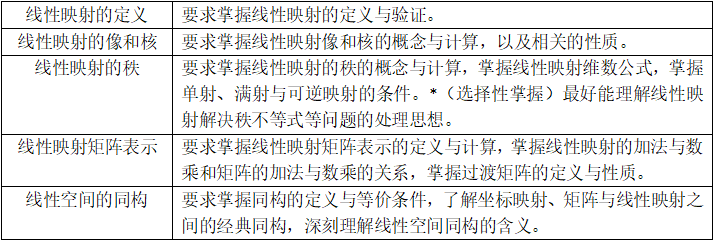
\includegraphics[scale=0.58]{2.png}
\end{figure}

\section{线性映射的定义}
\subsection{线性映射的定义}
\begin{definition}
	从线性空间$V_1(\mathbf{F})$到$V_2(\mathbf{F})$的一个映射$\sigma$是线性的,
	如果$\forall \alpha,\beta \in V_1$和$\forall \lambda,\mu \in \mathbf{F}$都有
	\begin{equation}
		\sigma(\lambda\alpha+\mu\beta)=\lambda\sigma(\alpha)+\mu\sigma(\beta).
	\end{equation}
	
	从线性空间$V$到自身的线性映射$\sigma$也叫作$V$上的线性变换,
	从线性空间$V(\mathbf{F})$到域$\mathbf{F}$的线性映射$f$叫作$V$上的线性函数(线性形式).
\end{definition}
实际上,上述定义式(1)可以分拆为以下(2)(3)式:
\begin{equation}
	\sigma(\alpha+\beta)=\sigma(\alpha)+\sigma(\beta)
\end{equation}
\begin{equation}
	\sigma(\lambda\alpha)=\lambda\sigma(\alpha)
\end{equation}
其中(2)称为加性,(3)称为齐次性.

根据定义,我们容易知道熟悉的过原点的直线(一次函数)是线性映射,而不过原点的直线不代表线性映射。

特别注意:根据定义,线性映射一定将出发空间的零元映射到到达空间的零元,
这是一个映射为线性映射的必要条件。
\subsection{线性映射的基本运算}
本节介绍线性映射的加法、数乘的定义,并介绍线性映射乘法(即复合)和逆运算。

我们需要首先说明一个记号,我们把线性空间$V_1(\mathbf{F})$到$V_2(\mathbf{F})$的所有线性映射组成的集合记作$L(V_1,V_2)$.
我们希望在这个集合上定义线性空间,于是需要定义其中元素(线性映射)的加法和数乘运算:
\begin{definition}
	设$\sigma,\ \tau\in L(V_1,V_2)$,规定$\sigma$与$\tau$之和及$\lambda$与
	$\sigma$的数乘$\lambda\sigma$分别为
	\begin{equation}
		(\sigma+\tau)(\alpha)=\sigma(\alpha)+\tau(\alpha),\ \forall\alpha\in V_1
	\end{equation}
	\begin{equation}
		(\lambda\sigma)(\alpha)=\lambda(\sigma(\alpha)),\ \forall\alpha\in V_1
	\end{equation}
\end{definition}
\begin{example}
	证明:$L(V_1,V_2)$与上述定义的线性映射加法和数乘构成域$\mathbf{F}$上的线性空间.
\end{example}
下面讨论线性映射的复合。设$\sigma \in L(V_1,V_2),\ \tau \in L(V_2,V_3)$,则$\tau\sigma$是$L(V_1,V_3)$
中的元素,且$\tau\sigma(\alpha)=\tau(\sigma(\alpha)),\ \forall \alpha \in V_1$.
\begin{example}
	证明:上述定义的映射$\tau\sigma$是线性映射.
\end{example}
注意:在上述定义中一定注意$\sigma$和$\tau$的顺序,我们需要先使用$\sigma$将$V_1$中的元素映射到
$V_2$,然后再用外层的$\tau$映射到$V_3$。

下面定义逆映射。如果可逆映射$\sigma:V_1 \to V_2$的逆映射为$\sigma^{-1}$,则$\sigma^{-1}\sigma=I_{V_1}$且
$\sigma\sigma^{-1}=I_{V_2}$。其中$I_{V}$的含义为$V$上的恒等映射,即$I_V(\alpha)=\alpha,\ \forall \alpha \in V$。
\begin{example}
	证明:上述定义的逆映射$\sigma^{-1}$为线性映射.
\end{example}
\subsection{线性映射举例}
本节内容希望各位同学按照教材3.1节例1-9了解常见的线性映射,了解一定的几何意义(虽然不会直接考察,但是对理解有帮助)。
其中例1、7、8、9希望同学们当做练习,例2中旋转变换的矩阵表示的求幂在矩阵计算专题中有提及,
例3镜面变换本是重点,但今年不要求内积空间,例6投影变换将在幂等矩阵中我们会再次提及。
\subsection{线性映射的确定}
有限维空间上的线性映射被基上的像唯一确定,即
\begin{theorem}
	已知线性映射$\sigma,\tau\in L(V_1,V_2)$,且有$V_1$的基$B=\{\alpha_1,\alpha_2,\cdots,\alpha_n\}$,
	若$\sigma(\alpha_i)=\tau(\alpha_i),\ \forall \alpha_i \in B$,则有$\sigma=\tau$.
\end{theorem}
即映射在一组基上的像确定了,则映射是唯一的。这一证明是容易的,希望同学自行尝试。
进一步地,我们有如下定理:
\begin{theorem}
	设$B=\{\alpha_1,\alpha_2,\cdots,\alpha_n\}$是$V_1(\mathrm{T})$的基,$S=\{\beta_1,\beta_2,\cdots,\beta_n\}$
	是$V_2$中任意$n$个向量,则存在唯一的$\sigma\in L(V_1,V_2)$使得$\sigma(\alpha_i)=\beta_i,\ i=1,2,\cdots,n$.
\end{theorem}
这一定理即教材定理3.6,希望同学们自己先尝试自己证明,只需先定义映射然后证明其线性性即可,唯一性在上一个定理中已经说明。
\subsection{习题}
\centerline{\heiti A组}
\begin{enumerate}
	\item 写出下列映射的出发空间和到达空间,并判断其是否为线性映射:
	
	(1)$\sigma(x_1,x_2)=(x_1-x_2,x_1,x_1+x_2)$;

	(2)$\sigma(x_1,x_2)=(x_1x_2,x_1+x_2)$;

	(3)$\sigma(p(x))=p(x+1)-p(x),\ \forall p(x) \in \mathbf{R}[x]_n$;

	(4)$\sigma(p(x))=p(a),\ \forall p(x)$,其中$a$为常数;

	(5)$\sigma(\xi)=2\xi+\xi_0$,其中$\xi$是线性空间$V$中的一个固定向量.
	\item 设$\sigma,\tau \in L(V,V)$且$\sigma^2=\sigma$,$\tau^2=\tau$,证明:
	
	(1)$\sigma^k=\sigma$(幂等变换);

	(2)若$(\sigma+\tau)^2=\sigma+\tau$,则$\sigma\tau=\theta$(零变换);

	(3)设$\sigma\tau=\tau\sigma$,则$(\sigma+\tau-\sigma\tau)^2=\sigma+\tau-\sigma\tau$.
	\item 是否存在$\mathbf{R}^3$到$\mathbf{R}^2$的线性映射$\sigma$使得$\sigma(1,-1,1)=(1,0)$,
	$\sigma(1,1,1)=(0,1)$.
\end{enumerate}
\centerline{\heiti B组}
\begin{enumerate}
	\item 已知
	$$\alpha_1=(1,-1),\alpha_2=(2,-1),\alpha_3=(-3,2);$$
	$$\beta_1=(1,0),\beta_2=(0,1),\beta_3=(1,1).$$
	是否存在$\sigma\in L(\mathbf{R}^2,\mathbf{R}^2)$,使得$\sigma(\alpha_i)=\beta_i(i=1,2,3)$.
	\item 设$\{\alpha_1,\alpha_2\}$是线性空间$V(\mathbf{F})$的一组基,$x_1\alpha_1+x_2\alpha_2 \in V$,
	定义$T(x_1\alpha_1+x_2\alpha_2)=r_1x_1\alpha_1+r_2x_2\alpha_2$,其中$r_1,r_2$是域$F$中的两个常数,
	证明:$T$是$V$上的一个线性变换,当$V=\mathbf{R}^2$时,说明$T$的几何意义.
	\item 已知$\mathbf{R}$上的线性变换$\sigma(x_1,x_2)=(x_1-x_2,x_1+x_2)$,$\tau(x_1,x_2)=(x_1-x_2,x_1-x_2)$.
	
	(1)求$\sigma^2(x_1,x_2)$;

	(2)$\sigma$是否可逆?如可逆,求$\sigma^{-1}(x_1,x_2)$;

	(3)求$\xi\in L(\mathbf{R}^2,\mathbf{R}^2)$,使得$\xi\tau=\theta$(零变换).
	\item 设$A,B,C,D \in \mathbf{F}^{n \times n}$,若
	$$T:X \to AXB+CX+XD,\ \forall X \in \mathbf{F}^{n \times n}.$$
	证明:

	(1)$T$为$\mathbf{F}^{n \times n}$上的线性变换;

	(2)当$C=D=0$时,$T$可逆的充要条件是$|AB| \neq 0$.
\end{enumerate}
\centerline{\heiti C组}
\begin{enumerate}
	\item 设 $V(\mathbf{F})$ 是一个 $n$ 维线性空间,$\sigma \in L(V,\ V)$,证明:

	(1)在 $\mathbf{F}[x]$ 中有一个次数不高于 $n^2$ 的多项式 $p(x)$ 使 $p(\sigma)=0$;
	
	(2)$\sigma$ 可逆$\iff$有一常数项不为 $0$ 的多项式 $p(x)$ 使 $p(\sigma)=0$。
\end{enumerate}

\section{线性映射的像、核与秩}
\subsection{线性映射的像和核的定义}
\begin{definition}
	设$\sigma$是线性空间$V_1(\mathbf{F})$到$V_2(\mathbf{F})$的线性映射,$V_1$的所有元素
	在$\sigma$下的像组成的集合
	$$\sigma(V_1)=\{\beta\ |\ \beta=\sigma(\alpha),\ \alpha \in V_1\}$$
	称为$\sigma$的像(或值域),记作$\textup{Im }\sigma$,$V_2$的零元$0_2$在$\sigma$下的完全原像
	$$\sigma^{-1}(0_2)=\{\alpha\ |\ \sigma(\alpha)=0_2,\ \alpha \in V_!\}$$
	称为$\sigma$的核,记作$\ker \sigma$.
\end{definition}
注意核的定义中$0_2$代表$V_2$中的零元,实际上下标也可以省略。

注意,线性映射的像和核分别是$V_2$和$V_1$的子空间。同样地,若$W_1$和$W_2$分别是$V_1$和$V_2$的
子空间,则$\sigma(W_1)$和$\sigma^{-1}(W_2)$也分别是$V_2$和$V_1$的子空间。以上命题的证明很简单,各位可以自行尝试。

下面是一种经典题型,即已知线性映射求线性映射的像和核,注意方法如下:

1. 像空间$\textup{Im }\sigma=\sigma(V_1)=L(\sigma(\alpha_1),\sigma(\alpha_2),\cdots,\sigma(\alpha_n))$,即线性映射在
一组基下的像的线性扩张,解答写出极大线性无关组然后扩张即可;

2. 核空间直接令$\sigma(\alpha)=0$,利用解线性方程组得到解$\alpha$,结果的线性扩张即为核空间。
\begin{example}
	已知$\mathbf{R}^3$到$\mathbf{R}^2$的映射$\sigma$为$\sigma(x_1,x_2,x_3)=(x_1+x_2,x_2-x_3)$,
	求$\sigma$的像和核.
\end{example}
\subsection{线性映射的秩的定义}
我们已知$\textup{Im }\sigma=\sigma(V_1)=L(\sigma(\alpha_1),\sigma(\alpha_2),\cdots,\sigma(\alpha_n))$,
我们基于此定义线性映射的秩:
\begin{definition}
	设$\sigma\in L(V_1,V_2)$,如果$\sigma(V_1)$是$V_2$的有限维子空间,则
	$\sigma(V_1)$的维数称为$\sigma$的秩,记作$r(\sigma)$,即$r(\sigma)=\dim \sigma(V_1)$.
\end{definition}
简单理解即线性映射的秩即为线性映射像空间的维数。
\subsection{线性映射基本定理(维数公式)}
这一定理是本学期最重要的定理之一,因其重要性也被冠以线性映射基本定理(有线维线性空间)的名号:
\begin{theorem}
	设$\sigma \in L(V_1,V_2)$,若$\dim V_1=n$,则
	$$r(\sigma)+\dim\ker\sigma=n.$$
\end{theorem}
这一定理的证明方式希望大家熟练掌握,下面是一个思想上类似的例子:
\begin{example}
	设$\sigma$为有限维线性空间$V$上的线性变换,$W$是$V$的子空间,证明:
	$$\dim\sigma(W)+\dim(\sigma^{-1}(0) \cap W)=\dim W.$$
\end{example}
基于线性映射基本定理,我们可以得到如下定理:
\begin{theorem}
	对$\sigma \in L(V_1,V_2)$且$\dim V_1=\dim V_2=n$,我们有
	$\ker\sigma=\{0\}\iff \sigma$为单射$\iff \sigma$为满射$\iff \sigma$为双射(可逆)$\iff r(\sigma)=n$(满秩).
\end{theorem}
显然这一定理前提适用于一切有限维空间上的线性变换。我们需要注意的是,上述第一个等价式不是基于线性映射基本定理得到的,
是教材定理3.1的内容,证明较为容易,建议先自己尝试证明。

线性映射基本定理还隐藏着一个结论,即不可能存在从低维空间到高维空间的满射(反证法代入维数公式即可,当然也可以利用线性相关性证明)。
\subsection{线性映射的像和核的进一步讨论}
\textbf{注:本节内容如果时间不够可以快速略过,只需大致了解重要原则以及结论即可。}

关于线性变换的像和核有很多的包含关系或等式等结论,实际上很多问题都来源于线性映射基本定理及其推论,本节我们主要探讨这一话题。

我们首先说明几个重要的原则:

1. 解决此类问题大多需要综合利用维数公式及其推论,需要讲题给条件转化为合适的等价表述然后解决;

2. 注意集合相等的证明方式,实际上就是两个集合互相包含。实际上很多时候一边的包含是显然的,只需证明另一边;

3. 时刻注意线性映射的像和核的定义,线性空间的交、和与直和的概念,例如看到像需要想到其存在原像,看到和与直和要想到将向量分拆等。

接下来我们看一些经典的结论(已知$V$为有限维线性空间,$\sigma\in L(V,V)$),有余力的同学可以思考其证明,其中结论1最为常见:

1. 若$\sigma$为幂等变换(即$\sigma^2=\sigma$)有$V=\ker\sigma\oplus\textup{Im }\sigma$;

2. $r(\sigma^2)=r(\sigma) \iff V=\ker\sigma\oplus\textup{Im }\sigma$;

3. $\ker\sigma=\ker\sigma^2 \iff \ker\sigma \cap \textup{Im }\sigma=\{0\} \iff \textup{Im }\sigma=\textup{Im }\sigma^2 \iff V=\ker\sigma\oplus \textup{Im }\sigma$;

4. $\ker\sigma \subseteq \ker\sigma^2 \subseteq \ker\sigma^3 \subseteq \cdots$;

5. $\textup{Im }\sigma \supseteq \textup{Im }\sigma^2 \supseteq \textup{Im }\sigma^3 \supseteq \cdots$;

6. 存在正整数$m$使得对任意的$n>m$都有$\ker\sigma^n=\ker\sigma^m$,$\textup{Im }\sigma^n=\textup{Im }\sigma^m$;

7. 存在正整数$m$使得$V=\textup{Im }\sigma^m+\ker\sigma^m$;

8. $\dim(\ker\sigma+\textup{Im }\sigma) \ge \cfrac{n}{2}$,等号成立充要条件为$\ker\sigma=\textup{Im }\sigma$.
\subsection{习题}
\centerline{\heiti A组}
\begin{enumerate}
	\item 是否存在$\mathbf{R}^2$到$\mathbf{R}^3$的线性映射$\sigma$使得$\sigma(3,2)=(1,0,0)$,$\sigma(1,5)=(1,1,0)$,$\sigma(-1,4)=(1,1,1)$.
	\item 求$\sigma(x_1,x_2,\cdots,x_n)=(x_1,0,\cdots,0)$的像、核与秩.
\end{enumerate}
\centerline{\heiti B组}
\begin{enumerate}
	\item 已知$\mathbf{R}^3$上的两个线性变换$\sigma,\tau$为:
	$$\sigma(x_1,x_2,x_3)=(x_3,0,0),$$
	$$\tau(x_1,x_2,x_3)=(x_1+x_2+x_3,x_1-x_2,0).$$
	(1)求$r(\sigma)$,$r(\tau)$,$\textup{Im }\sigma$,$\ker\sigma$;

	(2)求$r(\tau\sigma)$,$r(\sigma\tau)$,$r(\sigma+\tau)$;

	(3)求$\textup{Im }\tau+\ker\tau$.
	\item 设$\sigma(p(x))=p'(x)$(求导),$\forall p(x) \in \mathbf{R}[x]_n$.
	
	(1)证明:$\sigma$是$\mathbf{R}[x]_n$上的线性变换;

	(2)求$\sigma$的值域和$r(\sigma)$,说明$\sigma$是否可逆;

	(3)求$\sigma$的核及其维数;

	(4)求$r(\sigma)+\dim\ker\sigma$,问:$\mathbf{R}[x]_n=\ker\sigma+\textup{Im }\sigma$是否成立.
	\item 设$V$为有限维线性空间,$T\in L(V,V)$且$T$不是恒等变换也不是零变换,问:下列情况是否可能发生,
	如果可能请举例,不可能请说明理由.

	(1)$\textup{Im }T \cap \ker T = \{0\}$;

	(2)$\textup{Im }T \subset \ker T$;

	(3)$\ker T = \textup{Im }T$;

	(4)$\ker T \subset \textup{Im }T$.
	\item 若$\sigma_1,\sigma_2\in L(V,V)$,判断下列说法是否正确,正确请给出证明,反之给出反例:
	
	(1)由$r(\sigma)+\dim\ker\sigma=n$可知$V=\ker\sigma+\textup{Im }\sigma$;

	(2)若有$\textup{Im }T \cap \ker T = \{0\}$,则$V=\ker\sigma+\textup{Im }\sigma$成立;

	(3)因为$\forall \alpha \in V$有$(\sigma_1+\sigma_2)(\alpha)=\sigma_1(\alpha)+\sigma_2(\alpha)$,
	所以$(\sigma_1+\sigma_2)(V)=\sigma_1(V)+\sigma_2(V)$;

	(4)$(I-\sigma)(V)+\sigma(V)=V$($I$为恒等映射).
	\item 已知$V$为有限维线性空间,$\sigma\in L(V,V)$,且$\ker\sigma=\textup{Im }\sigma$,证明:
	
	(1)$n$为偶数;

	(2)存在$V$的一组基$\alpha_1,\cdots,\alpha_n$使得
	$$\sigma(\alpha_1,\cdots,\alpha_n)=(\alpha_1,\cdots,\alpha_n)\begin{pmatrix}
		0 & E_{\frac{n}{2}} \\ 0 & 0
	\end{pmatrix}.$$
\end{enumerate}
\centerline{\heiti C组}
\begin{enumerate}
	\item 设$V$是一个$n$维线性空间,$V=W_1\oplus W_2$,$\sigma\in L(V,V)$,证明:$\sigma$可逆$\iff V=\sigma(W_1)+\sigma(W_2)$.
	\item 设$V_1,V_2,V_3$分别为$m,n,s$维线性空间,$\sigma\in L(V_1,V_2),\tau\in L(V_2,V_3)$,则
	$$r(\sigma)+r(\tau)-n \le r(\tau\sigma) \le \min(r(\sigma),r(\tau)).$$
	\item 设$V_1$是有线维线性空间,$\sigma,\tau\in L(V_1,V_2)$,则
	$$r(\sigma+\tau) \le r(\sigma)+r(\tau).$$
	
	事实上前两题的结论在下一章节矩阵的秩中都会涉及,此处有兴趣的同学可以尝试从线性映射的角度理解这两个秩不等式.
	由于这是教材中小字部分内容,一般而言不在考察范围,如果出现且无法找到合适方式,可以考虑化为矩阵进行证明.
	\item 设$\sigma\in L(V,V)$,$\dim V_1=n$,且$\sigma^2=\sigma$,$I$是$V$上的恒等变换,证明:
	
	(1)$(I-\sigma)(V) \in \ker\sigma$;

	(2)$r(I-\sigma)+r(\sigma)=n$.
	\item 已知$V$为有限维线性空间,$\sigma\in L(V,V)$,且$\sigma^2=\theta$(零映射),证明:
	
	(1)$\sigma$的像空间维数不超过$\cfrac{n}{2}$;

	(2)设$A$是$\sigma$在某组基下的矩阵,则方程组$AX=0$的基础解系至少有$\cfrac{n}{2}$个解.
\end{enumerate}

\section{线性映射矩阵表示}
\subsection{一个最基本的定义}
\begin{definition}
	设$B_1=\{\epsilon_1,\epsilon_2,\dots,\epsilon_n\}$是$V_1(F)$的基,$B_2=\{\alpha_1,\alpha_2,\cdots,\alpha_m\}$是$V_2(F)$的基,
	则线性映射$\sigma \in L(V_1,V_2)$被它作用于基$B_1$的像
	$$\sigma(B_1)=\{\sigma(\epsilon_1),\sigma(\epsilon_2),\dots,\sigma(\epsilon_n)\}$$
	所唯一确定,而$\sigma(B_1)$是$V_2$的一个子集,于是
	$$\begin{cases}
		\sigma(\epsilon_1)=a_{11}\alpha_1+a_{21}\alpha_2+\cdots+a_{m1}\alpha_m \\
		\sigma(\epsilon_2)=a_{12}\alpha_1+a_{22}\alpha_2+\cdots+a_{m2}\alpha_m \\
		\cdots \\
		\sigma(\epsilon_n)=a_{1n}\alpha_1+a_{2n}\alpha_2+\cdots+a_{mn}\alpha_m
	\end{cases}.$$
	我们将$\sigma(B_1)=\{\sigma(\epsilon_1),\sigma(\epsilon_2),\dots,\sigma(\epsilon_n)\}$
	关于基$B_2$的坐标排列成矩阵$M(\sigma)$,即
	$$M(\sigma)=\begin{pmatrix}
		a_{11} & a_{12} & \cdots & a_{1n} \\
		a_{21} & a_{22} & \cdots & a_{2n} \\
		\cdots & \cdots &        & \cdots \\
		a_{m1} & a_{m2} & \cdots & a_{mn}
	\end{pmatrix}.$$
\end{definition}
更通俗来说,线性映射矩阵表示就是将线性映射在一组基上的像在另一组基下的坐标按列排列的结果。

之后我们会经常看见两种记号,即$(\sigma(\epsilon_1),\sigma(\epsilon_2),\dots,\sigma(\epsilon_n))$ 
和$\sigma(\epsilon_1,\epsilon_2,\dots,\epsilon_n)$。实际上是等价的,等价原因是
$(\sigma(\epsilon_1),\sigma(\epsilon_2),\dots,\sigma(\epsilon_n))A=(\sigma(\epsilon_1,\epsilon_2,\dots,\epsilon_n))A=\sigma((\epsilon_1,\epsilon_2,\dots,\epsilon_n)A)$成立,
这一性质在之后会有运用,证明并不复杂,可以自行尝试或参考我的矩阵辅学授课。

除此之外,我们还应当强调以下结论,在我们后续研究线性方程组解的相关性质时是常用的:
\begin{theorem}
	线性映射是单射当且仅当其矩阵表示为列满秩矩阵,线性映射是满射当且仅当其矩阵表示为行满秩矩阵.
\end{theorem}
这一结论的证明比较基本,希望大家能透过这一个结论看到列满秩矩阵与行满秩矩阵更本质的特征。
\subsection{一组简单的例子}
\begin{example}
	已知$\sigma \in L(\mathbf{R}^3,\mathbf{R}^3)$且$\sigma(x_1,x_2,x_3)=(x_1+x_2,x_1-x_3, x_2)$
	
	\textup{(1)}求$\sigma$的像空间和核空间;

	\textup{(2)}求$\sigma$关于$\mathbf{R}^3$自然基的矩阵.
\end{example}

\begin{example}
	设$A=\begin{pmatrix}1 & 0 & 2 \\ -1 & 2 & 1 \\ 1 & 2 & 5\end{pmatrix}$为两个三维线性空间之间的线性映射$\sigma$对应的矩阵,
	求$\sigma$的像空间和核空间.
\end{example}

\begin{example}
	已知$3$阶矩阵$A=\begin{pmatrix}
		1 & 0 & 1 \\ 0 & -1 & 0 \\ -1 & 1 & -1
	\end{pmatrix}$,定义$\mathbf{F}^{3 \times 3}$上的线性变换$\sigma(X)=AX,\ X \in \mathbf{F}^{3 \times 3}$,
	求$\sigma$的像和核.
\end{example}
实际上,例题2.4.1和2.4.3都是属于已知映射求像和核的题目,具体方法在像和核一节已经讲述,并且求矩阵表示也是根据上面的定义
即可,都是程式化的。然而例7则有不同,但此题与例2.4.1、2.4.2也有关联。实际上
此类问题像空间就是以矩阵列空间为坐标的向量的线性扩张,核空间是以矩阵零空间的基(即$AX=0$的基础解系)为坐标的向量的线性扩张,
推导见例7解析或我的矩阵辅学,希望各位同学能掌握推导并理解这三个例题之间的关系与区别。

\subsection{习题}
\centerline{\heiti B组}
\begin{enumerate}
	\item 已知$f_1=1-x,f_2=1+x^2,f_3=x+2x^2$是$\mathbf{R}[x]_3$中三个元素,$\sigma$是$\mathbf{R}[x]_3$
	上的线性变换且满足$\sigma(f_1)=2+x^2,\sigma(f_2)=x,\sigma(f_3)=1+x+x^2$.

	(1)证明:$f_1,f_2,f_3$构成$\mathbf{R}[x]_3$的一组基;

	(2)求$\sigma$在基$\{f_1,f_2,f_3\}$下的矩阵;

	(3)设$f=1+2x+3x^2$,求$\sigma(f)$.
	\item 设$V=M_2(\mathbf{R})$是$\mathbf{R}$上所有$2 \times 2$矩阵构成的实数域上的线性空间,
	已知
	$$A=\begin{pmatrix}1 & -1 \\ \lambda & 1 \end{pmatrix}(\lambda \in \mathbf{R}),\ \ B=\begin{pmatrix}1 & 2 \\ -1 & -1 \end{pmatrix}$$

	\textup{(1)}证明:$\phi(X)=AXB$为$V$上的线性变换;

	\textup{(2)}证明:$\lambda\neq-1$时,$\phi$为可逆线性变换;

	\textup{(3)}$\lambda=-1$时,求$\phi$的像空间和核空间;

	\textup{(4)}将\textup{(3)}中的值域扩充为$V$的一组基,并求$\phi$在这组基下的矩阵.
	\item 设矩阵空间$\mathbf{R}^{2\times 2}$的子空间为
	$$V=\{X=(x_{ij})_{2\times 2}\ |\ x_{11}+x_{12}+x_{21}=0,\ x_{ij}\in \mathbf{R}\}$$
	V中的线性变换为$\sigma(X)=X+X^\mathrm{T}$,求$V$的一组基,使得$\sigma$在该基下的矩阵表示为对角矩阵.
	\item 设 $\mathbf{R}[x]_4$ 是数域 $\mathbf{R}$ 上次数小于 $4$ 的多项式所构成的线性空间 ( 约定零多项式次数为 $-\infty$ )。$M_2(\mathbf{R})$ 是 $\mathbf{R}$ 上 $2$ 阶方阵所构成的线性空间,定义 $T : \mathbf{R}[x]_4 \to M_2(\mathbf{R})$ 如下,对 $f(x) \in \mathbf{R}[x]_4$,

	$$
	T(f(x))=\begin{pmatrix}f(0) & f(1) \\ f(-1) & f(0)\end{pmatrix}
	$$
	
	\textup{(1)}求出 $T$ 的核空间 $N(T)$ 和像空间 $R(T)$;
	
	\textup{(2)}求$T$在$\mathbf{R}[x]_4$和$M_2(\mathbf{R})$的基下的矩阵表示.
\end{enumerate}
\centerline{\heiti C组}
\begin{enumerate}
	\item 设矩阵$A \in \mathbf{F}^{m \times n}$,$A$的秩$r(A)=r$,定义$\mathbf{F}^{n \times p}$到$\mathbf{F}^{m \times p}$的线性映射
	$\sigma$,使得$\forall X \in \mathbf{F}^{n \times p}$,$\sigma(X)=AX$.求$\sigma$核空间的维数.
	\item 设$V$为数域$\mathbf{F}$上的线性空间,称$L(V,\mathbf{F})$(所有$V$到$\mathbf{F}$的线性映射构成的线性空间)
	为$V$的对偶空间,记为$V'$。若$T \in L(V,W)$,则$T$的对偶映射是$T' \in L(W',V')$:对于$\phi \in V'$,
	$T'(\phi)=\phi T$.

	\textup{(1)}设$v_1,v_2,\dots,v_n$是$V$的基,则$v_1,v_2,\dots,v_n$的对偶基是$V'$中的元素组$\phi_1,\dots,\phi_n$,
	其中每个$\phi_j$都是$L(V,\mathbf{F})$中的元素,使得
	$$\phi_j(v_k)=\begin{cases}
		1 & k=j \\ 0 & k \neq j
	\end{cases}$$
	试证明对偶基是对偶空间的基;

	\textup{(2)}证明对偶映射是线性映射,并证明$\forall T \in L(U,V)$,$S \in L(V,W)$,$(ST)'=T'S'$;

	\textup{(3)}证明$\dim \ker(T')=\dim \ker(T)+\dim W-\dim V$;

	\textup{(4)}证明$\dim \textup{Im}(T)=\dim \textup{Im}(T')$;

	\textup{(5)}证明$T$是单射等价于$T'$是满射,$T$是满射等价于$T'$是单射;

	\textup{(6)}证明$T'$的矩阵是$T$的转置.
\end{enumerate}
\section{线性空间的同构}
\subsection{线性空间同构的概念}
\begin{definition}
	如果由线性空间$V_(\mathbf{F})$到$V_2(\mathbf{F})$存在一个线性双射$\sigma$,则称
	$V_(\mathbf{F})$和$V_2(\mathbf{F})$是同构的,记作$V_1(\mathbf{F}) \cong V_2(\mathbf{F})$,
	$\sigma$称为$V_(\mathbf{F})$到$V_2(\mathbf{F})$的一个同构映射.
\end{definition}
容易验证同构为等价关系,且对上述同构映射$\sigma$,$V_1$中向量组$\{\alpha_1,\alpha_2,\cdots,\alpha_m\}$与$V_2$中对应的
$\{\sigma(\alpha_1),\sigma(\alpha_2),\cdots,\sigma(\alpha_m)\}$有相同的线性相关性,这不难证明。

下面是同构的等价条件:
\begin{theorem}
	两个线性空间$V_(\mathbf{F})$和$V_2(\mathbf{F})$同构的充要条件是它们的维数相等.
\end{theorem}
上述即教材定理3.8,定理的证明是简单的,利用维数公式以及同构是等价关系即可。

我们需要指出,同构是本教材中最重要的概念之一,它统一了教材2-3章所学的内容,
将线性空间可以按维数划分为不同的等价类,并且表明线性空间最本质的结构就在于
基及其维数,之前第二章研究的线性相关性与向量组的秩等就是研究线性空间的内部结构,
而线性映射则将相同或不同结构的线性空间联系在一起,同构则表明只要线性空间维数相同,
则可以将两个空间中的所有元素一一对应。
\subsection{线性空间同构举例}
在上一节最后我们提到,同构则表明只要线性空间维数相同,则可以将两个空间中的所有元素
一一对应。本节则研究几个经典的一一对应的例子。

1. 坐标映射:请回顾上一专题中向量的坐标,证明坐标映射是同构映射(实际上是显然的,因为一个
向量在一组基下坐标唯一,而一个坐标对应唯一一个向量);

2. 若$\dim V_1(\mathbf{F})=m$,$\dim V_2(\mathbf{F})=n$,则$L(V_1,V_2) \cong F^{m \times n}$。
证明有两种方式,一种来源于教材定理3.7,较为复杂,我们实际上只需要通过线性映射矩阵表示即可说明。

下面我们通过几个例题进一步了解几个常见的例子(简单题基本只需要判断维数是否相等即可):
\begin{example}
	指出下面各组内的两个线性空间是否同构,若同构可以进一步思考同构映射的构造:

	\textup{(1)}最高次不超过$n-1$的多项式构成的线性空间$\mathbf{R}[x]_n$与$\mathbf{R}^n$;

	\textup{(2)}全体复数在实数域上的线性空间$\mathbf{C}(\mathbf{R})$与$\mathbf{R}^2$;

	\textup{(3)}全体二元复向量$\mathbf{C}^2$在实数域上构成的线性空间$\mathbf{C}^2(\mathbf{R})$与$\mathbf{R}[x]_4$;

	\textup{(4)}全体二元复向量$\mathbf{C}^2$在复数域上构成的线性空间$\mathbf{C}^2(\mathbf{C})$与$L(\mathbf{R}^4,\mathbf{R})$.
\end{example}

\subsection{一些相似的定理}
\begin{theorem}
	\textbf{线性映射对向量坐标的影响}
	
	设$\sigma \in L(V_1,V_2)$关于$V_1$和$V_2$的基$B_1$和基$B_2$的矩阵为$A=(a_{ij})_{m \times n}$,
	且$\alpha$与$\sigma(\alpha)$在基$B_1$和基$B_2$下的坐标分别为$X$和$Y$,则$Y=AX$.
\end{theorem}
上述即教材定理4.1,这一定理给出一个向量经过线性映射之后,其坐标的变化。我们可以用下图表示:
\begin{figure}[h]
	\centering
	
\includegraphics[scale=0.75]{3.png}
\end{figure}

图中我们可以看出通过坐标映射后得到的新映射即为定理4.1描述的映射。

在描述下一定理之前,我们首先介绍过渡矩阵(变换矩阵)的概念。
\begin{definition}
	设$B_1=\{\alpha_1,\alpha_2,\cdots,\alpha_n\}$与$B_2=\{\beta_1,\beta_2,\cdots,\beta_n\}$是线性空间
	$V(\mathbf{F})$的任意两组基,$B_2$中每个基向量被基$B_1$表示为
	$$\begin{cases}
		\beta_1=a_{11}\alpha_1+a_{21}\alpha_2+\cdots+a_{n1}\alpha_n \\
		\beta_2=a_{12}\alpha_1+a_{22}\alpha_2+\cdots+a_{n2}\alpha_n \\
		\cdots \\
		\beta_n=a_{1n}\alpha_1+a_{2n}\alpha_2+\cdots+a_{nn}\alpha_n
	\end{cases}.$$
	将上式用矩阵表示为
	$$(\beta_1,\beta_2,\cdots,\beta_n)=(\alpha_1,\alpha_2,\cdots,\alpha_n)\begin{pmatrix}
		a_{11} & a_{12} & \cdots & a_{1n} \\
		a_{21} & a_{22} & \cdots & a_{2n} \\
		\cdots & \cdots &        & \cdots \\
		a_{n1} & a_{n2} & \cdots & a_{nn}
	\end{pmatrix}.$$
	我们将这一矩阵称为即$B_1$变为基$B_2$的变换矩阵(或过渡矩阵).
\end{definition}
简单而言就是将$B_2$中的向量在$B_1$下的坐标按列排列。需要注意表述中是$B_1$变为基$B_2$还是反过来,
这两个矩阵互逆。注意过渡矩阵一定是基与基之间的表示矩阵,并且过渡矩阵一定可逆。
\begin{theorem}
	\textbf{基的选择对向量坐标的影响}
	
	设线性空间$V$的两组基为$B_1$和$B_2$,且基$B_1$到$B_2$的变换矩阵(过渡矩阵)为$A$,如果
	$\xi \in V(F)$,且在$B_1$和$B_2$下的坐标分别为$X$和$Y$,则$Y=A^{-1}X$.
\end{theorem}
上述即教材定理4.10,描述同一个向量在不同基下坐标之间的关系。事实上,这与本节同构关系紧密,因为
同构意味着两个线性空间结构一致,故同构映射可以保持向量组的线性关系不变。在同构关系下,
线性组合对应线性组合,线性无关对应线性无关,线性相关对应线性相关。我们有如下定理:
\begin{theorem}
	设$(\alpha_1,\alpha_2,\cdots,\alpha_n)$是线性无关的向量组,且
	$$(\beta_1,\beta_2,\cdots,\beta_s)=(\alpha_1,\alpha_2,\cdots,\alpha_n)A,$$
	则向量组$(\beta_1,\beta_2,\cdots,\beta_s)$的秩等于矩阵$A$的秩.
\end{theorem}
定理的证明需要用到坐标映射是同构映射这一事实,我们不难发现等式左侧向量组与$A$的列向量组是等价的。
事实上我们也可以由此发现,过渡矩阵一定是可逆矩阵。
\begin{theorem}
	已知$\beta_i=a_{1i}\alpha_1+a_{2i}\alpha_2+\cdots+a_{ni}\alpha_n(i=1,2,\cdots,n)$,
	且$A=(a_{ij})$可逆,则$\alpha_1,\alpha_2,\cdots,\alpha_n$与$\beta_1,\beta_2,\cdots,\beta_n$
	是等价的.
\end{theorem}
实际上这一定理与上一定理的思想都是类似的,我们可以看一个例题练习一下:
\begin{example}
	已知$\beta_1=\alpha_2+\alpha_3$,$\beta_2=\alpha_1+\alpha_3$,$\beta_3=\alpha_1+\alpha_2$,
	证明$\alpha_1,\alpha_2,\alpha_3$与$\beta_1,\beta_2,\beta_3$等价.
\end{example}
\begin{theorem}
	\textbf{基的选择对映射矩阵的影响}
	
	设线性变换$\sigma \in L(V,V)$,$B_1=\{\alpha_1,\dots,\alpha_n\}$和$B_2=\{\beta_1,\dots,\beta_n\}$
	是线性空间的$V(F)$的两组基,基$B_1$变为基$B_2$的变换矩阵为$C$,如果$\sigma$在基$B_1$下的矩阵为$A$,
	则$\sigma$关于基$B_2$所对应的矩阵为$C^{-1}AC$.
\end{theorem}
上述即教材定理7.4,研究同一个映射在不同基下表示矩阵之间的关系。实际上我们将在下一专题初等矩阵一节进一步讨论。
这一定理的证明需要用到我们之前描述的两种线性映射矩阵表示的统一性。

\subsection{习题}
\centerline{\heiti A组}
\begin{enumerate}
	\item 给定$\mathbf{R}^4$的两组基
	$$\alpha_1=(1,1,1,1),\ \alpha_2=(1,1,-1,-1),\ \alpha_3=(1,-1,1,-1),\ \alpha_4=(1,-1,-1,1);$$
	$$\beta_1=(1,1,0,1),\beta_2=(2,1,3,1),\beta_3=(1,1,0,0),\beta_4=(0,1,-1,-1).$$
	求由基$\alpha_1,\alpha_2,\alpha_3,\alpha_4$到基$\beta_1,\beta_2,\beta_3,\beta_4$的
	过渡矩阵,并求向量$\xi=(1,0,0,-1)$在基$\alpha_1,\alpha_2,\alpha_3,\alpha_4$下的坐标.
\end{enumerate}
\centerline{\heiti B组}
\begin{enumerate}
	\item 设$B=\{\beta_1,\beta_2,\cdots,\beta_n\}$是实数域$\mathbf{R}$上的线性空间$V$的一组基,
	$T \in L(V)$,$T(\beta_1)=\beta_2,T(\beta_2)=\beta_3,\cdots,T(\beta_{n-1})=T(\beta_n),T(\beta_n)=\sum\limits_{i=1}^{n}a_i\beta_i(a_i \in \mathbf{R})$,
	求$T$关于基$B$的表示矩阵,并求在什么条件下$T$是同构映射.
	\item 设$V(\mathbf{R})$是线性空间,$\sigma$是$V(\mathbf{R})$到$R^3$的同构映射,且
	$\sigma(\alpha_1)=(1,0,1)$,$\sigma(\alpha_2)=(-2,1,0)$,$\sigma(\alpha_3)=(-3,2,1)$,$\sigma(\alpha_4)=(1,1,2)$.

	(1)$\alpha_1$在$L(\alpha_2,\alpha_3)$中吗;

	(2)设$W_1=L(\alpha_1,\alpha_2)$,$W_2=L(\alpha_3,\alpha_4)$,求$W_1\cap W_2$.
	\item 设$c_1,c_2,\cdots,c_n$是$n$个互异的实常数,证明:$\mathbf{R}[x]_n$到$\mathbf{R}$的一个映射$\sigma$:
	$$\sigma(p(x))=(p(c_1),p(c_2),\cdots,p(c_n))$$
	是$\mathbf{R}[x]_n$到$\mathbf{R}$的一个同构映射.
	\item 证明:当$n$为奇数时,$\alpha_1,\alpha_2,\cdots,\alpha_n$线性无关的充要条件是
	$\alpha_1+\alpha_2,\alpha_2+\alpha_3,\cdots,\alpha_n+\alpha_1$线性无关.
	\item 已知三维线性空间 $V$ 的线性变换 $\sigma$ 关于基 $\{\alpha_1,\ \alpha_2,\ \alpha_3\}$ 所对应的矩阵为

	$$
	\begin{pmatrix}1 & 2 & -1 \\ 2 & 1 & 0 \\ 3 & 0 & 1\end{pmatrix}
	$$
	
	\textup{(1)}求 $\sigma$ 在基 $\{\beta_1,\ \beta_2,\ \beta_3\}$ 下对应的矩阵 $B$,其中:
		$$
		\beta_1=2\alpha_1+\alpha_2+3\alpha_3,\ \beta_2=\alpha_1+\alpha_2+2\alpha_3,\ \beta_3=-\alpha_1+\alpha_2+\alpha_3
		$$
	
	\textup{(2)}求 $\sigma$ 的值域 $\sigma(V)$ 和核 $\textup{ker}\sigma$;
	
	\textup{(3)}把 $\sigma(V)$ 的基扩充为 $V$ 的基,并求 $\sigma$ 在这组基下对应的矩阵;
	
	\textup{(4)}把 $\textup{ker}\sigma$ 的基扩充为 $V$ 的基,并求 $\sigma$ 在这组基下对应的矩阵.
	\item 设
	$$B_1=\left\{\begin{pmatrix}
		1 & 0 \\ 0 & 0
	\end{pmatrix},\begin{pmatrix}
		0 & 1 \\ 0 & 0
	\end{pmatrix},\begin{pmatrix}
		0 & 0 \\ 1 & 0
	\end{pmatrix}\begin{pmatrix}
		0 & 0 \\ 0 & 1
	\end{pmatrix}\right\},$$
	$$B_2=\left\{\begin{pmatrix}
		1 & 0 \\ 0 & 0
	\end{pmatrix},\begin{pmatrix}
		1 & 1 \\ 0 & 0
	\end{pmatrix},\begin{pmatrix}
		1 & 1 \\ 1 & 0
	\end{pmatrix}\begin{pmatrix}
		1 & 1 \\ 1 & 1
	\end{pmatrix}\right\}.$$

	(1)证明:$B_2$也是线性空间$M_2(\mathbf{R})$的基;

	(2)求基$B_2$变为基$B_1$的变换矩阵;

	(3)求$M_2(\mathbf{R})$的一组基$B_3=\{A_1,A_2,A_3,A_4\}$,使得$A_i^2=A_i(i=1,2,3,4)$;

	(4)已知矩阵$A$关于基$B_2$的坐标为$(1,1,1,1)^\mathrm{T}$,求$A$关于基$B_3$的坐标.
\end{enumerate}
\centerline{\heiti C组}
\begin{enumerate}
	\item 设$A$是数域$\mathbf{F}$上的$n$阶可逆矩阵,把$A$和$A^{-1}$做如下分块:
	$$A=\begin{pmatrix}
		A_{11} & A_{12} \\ A_{21} & A_{22}
	\end{pmatrix},A^{-1}=\begin{pmatrix}
		B_{11} & B_{12} \\ B_{21} & B_{22}
	\end{pmatrix}$$
	其中$A_{11}$是$l \times k$矩阵,$B_{11}$是$k \times l$矩阵,
	$l$,$k$是小于$n$的正整数.用$W$表示$A_{12}X=0$的解空间,$U$表示$B_{12}Y=0$的解空间,
	其中$X$和$Y$为列向量,证明$W$与$U$同构.
	\item 设$K \subseteq F \subseteq E$是三个数域,已知$F$作为$K$上的线性空间是$n$维的,
	$E$作为$F$上的线性空间是$m$维的,证明:$E$作为$K$上的线性空间是$mn$维的.
\end{enumerate}
\chapter{矩阵运算\ 矩阵的秩}

\section{Overview}
\begin{figure}[h]
	\centering
	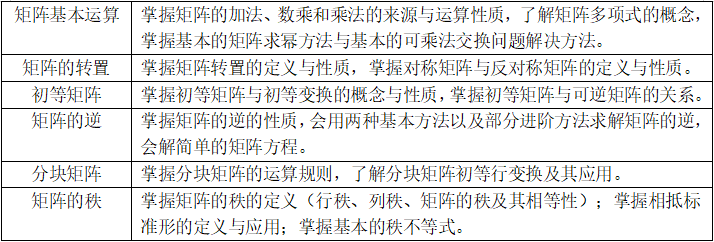
\includegraphics[scale=0.58]{4.png}
\end{figure}

\section{矩阵基本运算}
\subsection{基本概念}
\begin{enumerate}
	\item 矩阵的加法来源于线性映射的加法,矩阵相加要求两矩阵行列数一致,相加时只需对应位置元素相加即可;
	\item 矩阵的数乘来源于线性映射的数乘,计算只需矩阵的每个元素乘以常数即可;
	\item 矩阵的乘法来源于线性映射的复合,计算时要求前一个矩阵的列数等于后一个矩阵的行数,矩阵$A$与$B$
	相乘结果中第$i$行第$j$列元素为矩阵$A$的第$i$行与矩阵$B$的第$j$列对应位置元素相乘后求和的结果,
	即对于$A=(a_{ij})_{m \times n}$和$B=(b_{ij})_{n \times l}$,矩阵$C=AB=(c_ij)_{m \times l}$,且
	$c_{ij}=a_{i1}b_{1j}+a_{i2}b_{2j}+\cdots+a_{in}b_{nj},\ i=1,\cdot,m,j=1,\cdots,l$.
\end{enumerate}

\subsection{基本性质}
\begin{enumerate}
	\item 回顾上一专题中$m \times n$矩阵构成的线性空间$M_{m \times n}(\mathbf{F})$;
	\item 回顾矩阵乘法的基本性质:
	\begin{enumerate}
		\item $(AB)C=A(BC)$(结合律)
		\item $\lambda(AB)=(\lambda A)B=A(\lambda B)$(其中$\lambda$是数量)
		\item $A(B+C)=AB+AC$(左分配律)
		\item $(B+C)P=BP+CP$(右分配律)
		\item $A^kA^m=A^{k+m}$,$(A^k)^m=A^{km}$,其中$A$为方阵,$k$,$m$为任意整数,
		负整数对应于逆矩阵的情况。
	\end{enumerate}
	\item 回顾矩阵多项式的定义(利用线性映射多项式在基下的矩阵表示定义),
	并注意其交换性以及可因式分解性。
\end{enumerate}
\begin{example}
	展开矩阵多项式$(A+\lambda E)^n$.
\end{example}
\begin{example}
	设$f(x),\ g(x) \in \mathbf{F}[x]$,$A,\ B \in M_n(\mathbf{F})$,证明:
	$$f(A)g(A)=g(A)f(A);$$
	
	\textup{1. }如果$AB=BA$,则$f(A)g(B)=g(B)f(A)$\textup{;}

	\textup{2. }设$f(x)=1+x+\cdots+x^{m-1}$,$g(x)=1-x$,$A=\begin{pmatrix}
		a & b \\ 0 & a
	\end{pmatrix}$,计算$f(A)g(A)$.
\end{example}
其他需要注意的性质:
\begin{enumerate}
	\item 矩阵乘法不一定满足交换律(即$AB$不一定等于$BA$)。但是注意数量矩阵和任何矩阵相乘都是可交换的,因此求矩阵的幂次时,可以将其转化为$(A+\mu E)^n$(其中$E$为单位矩阵,$\mu$为常数)类型,然后利用二项式展开即可。很多情况下$A$都会是幂零矩阵,此时结果为有限项。
	\item $A\neq O$且$B\neq O$不能推出$AB\neq O$。例如线性方程组$AX = 0$有非零解,若$B$的各列均为方程非零解,则$AB = O$。
	\item 消去律也不一定满足:即$AC = BC$不一定$B = C$。原因在于$AB=AC \to A(B-C)=O$,由(2)可知不一定$B = C$。
\end{enumerate}

\subsection{矩阵可交换问题}
一般来说在本课程中此类问题直接设可交换矩阵的每一个元素都是未知数即可,一些特殊的技巧
(使用关于一些特殊形状矩阵的结论)以及涉及到之后才能学到的知识的方法我们在这里也不展开了。我们只讨论一个基本的技巧,即
$$\forall t,\ AB=BA \iff (A-tE)B=B(A-tE)$$
此处的$t$根据矩阵的对角线上元素来决定,原则是使得其余矩阵与$A-tE$相乘的计算过程更为简单(一般是使得0元素更多),这样解方程也会更轻松。
我们来看一个简单的例子:
\begin{example}
	求与矩阵$A=\begin{pmatrix}
		3 & 0 & 0 \\ -1 & 3 & 0 \\ 0 & -1 & 3
	\end{pmatrix}$可交换的矩阵.
\end{example}

关于可交换我们有以下定理,证明并不是很复杂(教材习题中有出现):
\begin{theorem}
	\textup{(1)}与主对角元两两互异的对角矩阵可交换的方阵只能是对角矩阵;

	\textup{(2)}准对角矩阵$A$每个对角分块内对角线元素相同,但不同对角块之间不同,则与$A$可交换的矩阵只能是准对角矩阵;
	
	\textup{(3)}与所有$n$级可逆矩阵可交换的矩阵为数量矩阵;
	
	\textup{(4)}与所有$n$级矩阵可交换的矩阵为数量矩阵.
\end{theorem}


\subsection{习题}
\centerline{\heiti A组}
\begin{enumerate}
	\item 证明:若$AB=BA$,$AC=CA$,则$A,\ B,\ C$为同阶方阵,且
	$$A(BC)=(BC)A,\ A(B+C)=(B+C)A.$$
	\item $A,\ B$都是$n$阶矩阵,求下列等式成立的充分条件:
	
	(1)$(A+B)^3=A^3+3A^2B+3AB^2+B^3$;

	(2)$(A+B)(A-B)=A^2-B^2$.
\end{enumerate}
\centerline{\heiti B组}
\begin{enumerate}
	\item 已知矩阵$A=\begin{pmatrix}
		1 & 0 & 4 \\ 0 & 1 & 2 \\ 0 & 1 & 2
	\end{pmatrix}$,求证:所有与$A$可交换的矩阵构成$M_3(\mathbf{R})$的一个子空间,并求子空间的一组基.
	\item 若$f(x)$是$x$的实系数$m$次多项式:
	$$f(x)=a_mx^m+a_{m-1}x^{m-1}+\cdots+a_1x+a_0,$$
	则有矩阵多项式:
	$$f(A)=a_mA^m+a_{m-1}A^{m-1}+\cdots+a_1A+a_0E\ (A^0=E).$$

	(1)若$A$为对角矩阵$B=\begin{pmatrix}
		\lambda_1 & 0 \\ 0 & \lambda_2
	\end{pmatrix}$,证明:$f(A)=\begin{pmatrix}
		f(\lambda_1) & 0 \\ 0 & f(\lambda_2)
	\end{pmatrix}$;

	(2)若$A=P^{-1}BP$,证明:$f(A)=Pf(B)P^{-1}$.
\end{enumerate}

\centerline{\heiti C组}
\begin{enumerate}
	\item 证明以下两个命题:
	
	(1)与矩阵$I=\begin{pmatrix}
		0 & 1 & 0 & \cdots & 0 & 0 \\
		0 & 0 & 1 & \cdots & 0 & 0 \\
		0 & 0 & 0 & \cdots & 0 & 0 \\
		\vdots & \vdots & \vdots &  & \vdots & \vdots \\
		0 & 0 & 0 & \cdots & 0 & 1 \\
		1 & 0 & 0 & \cdots & 0 & 0
	\end{pmatrix}$可交换的矩阵$A$都可以写成$I$的一个多项式,即
	$A=a_{11}E+a_{12}I+a_{13}I^2+\cdots+a_{1n}I^{n-1}$;
	
	(2)与矩阵$J=\begin{pmatrix}
		0 & 1 & 0 & \cdots & 0 & 0 \\
		0 & 0 & 1 & \cdots & 0 & 0 \\
		0 & 0 & 0 & \cdots & 0 & 0 \\
		\vdots & \vdots & \vdots &  & \vdots & \vdots \\
		0 & 0 & 0 & \cdots & 0 & 1 \\
		0 & 0 & 0 & \cdots & 0 & 0
	\end{pmatrix}$可交换的矩阵$A$都可以写成$J$的一个多项式,即
	$A=a_{11}E+a_{12}J+a_{13}J^2+\cdots+a_{1n}J^{n-1}$;
\end{enumerate}

\section{矩阵的转置}
\subsection{基本概念}
实际上,矩阵的转置就是第$i$行变成了第$i$列,或者抽象表达为:
$$A=(a_{ij})_{m \times n},\ A^\mathrm{T}=(a'_{ji})_{n \times m},\ a_{ij}=a'_{ji}$$
写成矩阵形式为:
\begin{definition}
	设$A=\begin{pmatrix}
		a_{11} & a_{12} & \cdots & a_{1n} \\
		a_{21} & a_{22} & \cdots & a_{2n} \\
		\vdots & \vdots &       & \vdots \\
		a_{m1} & a_{m2} & \cdots & a_{mn}
	\end{pmatrix}$,称$\begin{pmatrix}
		a_{11} & a_{21} & \cdots & a_{m1} \\
		a_{12} & a_{22} & \cdots & a_{m2} \\
		\vdots & \vdots &       & \vdots \\
		a_{1n} & a_{2n} & \cdots & a_{mn}
	\end{pmatrix}$为矩阵$A$的转置,记作$A^\mathrm{T}$.
\end{definition}

\subsection{基本性质}
1. $(A^\mathrm{T})^\mathrm{T}=A$

2. $(A+B)^\mathrm{T}=A^\mathrm{T}+B^\mathrm{T}$

3. $(\lambda A)^\mathrm{T}=\lambda A^\mathrm{T}$($\lambda$是数量)

4. $(AB)^\mathrm{T}=B^\mathrm{T}A^\mathrm{T}$,$(A_1A_2\cdots A_n)^\mathrm{T}=A_n^\mathrm{T}\cdots A_2^\mathrm{T}A_1^\mathrm{T}$

5. $(A^\mathrm{T})^{-1}=(A^{-1})^\mathrm{T}$

6. $(A^\mathrm{T})^m=(A^m)^\mathrm{T}$

以上证明大都是平凡的,可以自己尝试完成。
\subsection{对阵矩阵与反对称矩阵}
\begin{definition}
	设$A=(a_{ij})_{n \times n}$,如果$\forall i,j=1,2,\cdots$均有$a_{ij}=a_{ji}$,
	则称$A$为对称矩阵,若均有$a_{ij}=-a_{ji}$,则称$A$为反对称矩阵.
\end{definition}
易得$A$为对称矩阵的充要条件为$A=A^\mathrm{T}$,$A$为反对称矩阵的充要条件为$A=-A^\mathrm{T}$.
\begin{example}
	证明以下几点性质:
	
	\textup{1. }反对称矩阵主对角元均为$0$\textup{;}
	
	\textup{2. }$AA^\mathrm{T}$和$A^\mathrm{T}A$均为对称矩阵\textup{;}
	
	\textup{3. }设$A,\ B$为$n$阶对称和反对称矩阵,则$AB+BA$是反对称矩阵\textup{;}
	
	\textup{4. }对称矩阵的乘积不一定对称\textup{;}
	
	\textup{5. }可逆的对称(反对称)矩阵的逆矩阵也是对称(反对称)矩阵。
\end{example}

\subsection{习题}
\centerline{\heiti A组}
\begin{enumerate}
	\item 设$\alpha=(1,-1,2)^\mathrm{T},\ \beta=(2,1,1)^\mathrm{T},\ A=\alpha\beta^\mathrm{T}$,求$A^n$.
	\item 设$\alpha,\ \beta$为三维列向量,且$\alpha\beta^\mathrm{T}=
	\begin{pmatrix}-1 & 2 & 1 \\ 1 & -2 & -1 \\ 2 & -4 & -2\end{pmatrix}
	$,求$\alpha^\mathrm{T}\beta$.
\end{enumerate}
\centerline{\heiti B组}
\begin{enumerate}
	\item 设$A$为$n$阶实矩阵,且$A^\mathrm{T}A=O$,证明:$A=O$.
	\item 设 $V=\{(a_{ij})_{n \times n}\ |\ \forall i,\ j,\ a_{ij}=a_{ji}\}$
	
	(1)证明:$V$ 为 $F^{n \times n}$ 的子空间;
	
	(2)求  $V$ 的基和维数.
	\item 求矩阵$\begin{pmatrix}
		a & b & c & d \\ -b & a & d & -c \\ -c & -d & a & b \\ -d & c & -b & a
	\end{pmatrix}$的逆.
\end{enumerate}

\centerline{\heiti C组}
\begin{enumerate}
	\item $a,b,c,d$是四个实数,证明:$\begin{cases}
		a^2+b^2=1 \\ c^2+d^2=1 \\ ac+bd=0
	\end{cases}$成立的充分必要条件是$\begin{cases}
		a^2+c^2=1 \\ b^2+d^2=1 \\ ab+cd=0
	\end{cases}$.
\end{enumerate}

\section{初等矩阵}
\subsection{基本概念与性质}
\begin{definition}
	将单位矩阵$E$做一次初等变换得到的矩阵称为初等矩阵,与三种初等行、列变换对应的三类初等矩阵为:
	
	\textup{(1)}将单位矩阵第$i$行(或列)乘$c$,得到初等倍乘矩阵$E_i(c)$\textup{;}

	\textup{(2)}将单位矩阵第$i$行乘$c$加到第$j$行,或将第$j$列乘$c$加到第$i$列,得到初等倍加矩阵$E_{ij}(c)$\textup{;}

	\textup{(3)}将单位矩阵第$i,j$行(或列)对换,得到初等对换矩阵$E_{ij}$.
\end{definition}
请各位同学以矩阵形式写出以上三类矩阵。注意:

1. 倍加变化请一定注意$i$和$j$在行列的情况下的不同;

2. 三类矩阵不是三个矩阵,例如行列选择不唯一,常数选择不唯一;

3. 注意三种初等矩阵都是可逆的,且$E_i^{-1}(c)=E_i(\cfrac{1}{c})$,$E_{ij}^{-1}(c)=E_{ij}(-c)$,$E_{ij}^{-1}=E_{ij}$;

4. 三种初等矩阵的转置:$E_i^\mathrm{T}(c)=E_i(c)$,$E_{ij}^\mathrm{T}(c)=E_{ji}(c)$,$E_{ij}^\mathrm{T}=E_{ij}$;

初等矩阵大家非常关心为什么左乘代表行变换,右乘代表列变换。以右乘为例,我们来看矩阵$A$和$B$相乘的任一列结果。我们可以将矩阵$A$
按列做分块矩阵得到$(\alpha_1,\cdots,\alpha_n)$,$\alpha_i$即表示$A$的第$i$列。然后矩阵$B$的第$j$列为列向量$(x_1,\cdots,x_n)^\mathrm{T}$,
由于矩阵$A$与$B$相乘结果第$j$列就是$A$与$B$的第$j$列相乘结果(回顾矩阵乘法的计算方式),则有$B$的第$i$列等于
$x_1\alpha_1+\cdots+x_n\alpha_n$即为$A$的全部列向量的线性组合,故右乘矩阵$A$得到矩阵的任一列都是$A$的全部列向量的线性组合,
所以右乘可以代表列变换。注意我这里并没有限制矩阵$B$为初等矩阵或可逆矩阵。

实际上左乘表示行变换可以用类似方法说明,只需按行对$B$分块即可。这一思想是特别重要的,在很多时候如果我们意识到左右乘是对被乘矩阵的行列
重新线性组合,思路会清晰很多。

关于初等矩阵还有一个相当重要的定理:
\begin{theorem}
	任意可逆矩阵都可以被表示为若干个初等矩阵的乘积.
\end{theorem}
定理证明只需要回忆高斯消元法可以将可逆矩阵化为单位矩阵即可。

利用矩阵初等变换我们可以获得本学期需要学习的三个矩阵标准形,因此这一内容虽然很基本但是非常重要:
\begin{enumerate}
	\item 相抵矩阵:本章已学习的内容,在之后会详细说明;
	\item 相似矩阵:若$P$为初等矩阵,对矩阵做$P^{-1}AP$变换即可得到与$A$相似的矩阵;
	\item 相合矩阵:两个矩阵,其中一个可以通过做相同的初等行列变换的到另一个矩阵(若$P$为初等矩阵,
	$P^{\mathrm{T}}AP$就是对$A$做了一次相同的初等行列变换)。
\end{enumerate}
请同学们思考:如何从线性映射矩阵表示的角度理解初等变换与标准形的关系?在B组习题中将有练习进行体会
(实际上对矩阵表示的基做“初等变换”就是对表示矩阵做了初等变换,这两种变换行列方向不一致且矩阵互逆)。

\subsection{习题}
\centerline{\heiti A组}
\begin{enumerate}
	\item 设$A$为三阶矩阵,将A的第二列加到第一列得到矩阵$B$,再对调$B$的$2$、$3$行得到单位矩阵,
	令$P_1=\begin{pmatrix}1 & 0 & 0 \\ 1 & 1 & 0 \\ 0 & 0 & 1\end{pmatrix}$,
	$P_2=\begin{pmatrix}1 & 0 & 0 \\ 0 & 0 & 1 \\ 0 & 1 & 0\end{pmatrix}$,试用
	$P_1$和$P_2$表示$A$.
	\item 设$A$为可逆矩阵,将$A$的第$i$行和第$j$行对调得到矩阵$B$,证明矩阵$B$可逆并求$AB^{-1}$.
	\item 设$A$为三阶可逆矩阵,且$P^{-1}AP=\begin{pmatrix}1 & 0 & 0 \\ 0 & 1 & 0 \\ 0 & 0 & 2\end{pmatrix}$,
	其中$P=(\alpha_1,\alpha_2,\alpha_3)$,令$Q=(\alpha_1+\alpha_2,\alpha_2,\alpha_3)$,求$Q^{-1}AQ$.
\end{enumerate}
\centerline{\heiti B组}
\begin{enumerate}
	\item 已知$\mathbf{R}^3$的基$B_1=\{\alpha_1,\alpha_2,\alpha_3\}$变为基$B_2=\{\xi_1,\xi_2,\xi_3\}$的变换矩阵
	为$A=(a_{ij})_{3 \times 3}$,求:

	(1)基$B_3=\{\alpha_2,\alpha_1,\alpha_3\}$变为基$B_2$的变换矩阵;

	(2)基$B_4=\{-\alpha_1,\alpha_2,\alpha_3\}$变为基$B_2$的变换矩阵;

	(3)基$B_4$变为基$B_5=\{\xi_3,\xi_2,-\xi_1\}$的变换矩阵;

	(4)基$B_4$变为基$B_6=\{\xi_1+\xi_2,\xi_2+\xi_3,\xi_3+\xi_1\}$的变换矩阵.
	\item 设$P=\begin{pmatrix}
		1 & 1 & 0 \\ 0 & 1 & 0 \\ 0 & 0 & 0
	\end{pmatrix}$,$Q=\begin{pmatrix}
		0 & 0 \\ 1 & 0
	\end{pmatrix}$,定义$\mathbf{R}^{3\times 2}$上映射$\sigma(A)=PAQ$,

	(1)验证$\sigma$是线性映射;

	(2)求$\ker\sigma$和$\textup{Im }\sigma$;

	(3)求$\mathbf{R}^{3\times 2}$的两组基,使得$\sigma$关于这两组基的表示矩阵是对角矩阵.
\end{enumerate}

\section{可逆矩阵}
\subsection{基本概念}
\begin{definition}
	设$A \in M_n(\mathbf{F})$,如果存在$B \in M_n(\mathbf{F})$,使得$AB=BA=E$则称矩阵$A$可逆,
	并把$B$称为$A$的逆矩阵.
\end{definition}
注意,逆矩阵定义基于方阵,非方阵没有上述逆矩阵。广义逆矩阵允许非方阵,但那是另一个定义,
我们不需要掌握。对于可逆矩阵,注意以下两个定理:
\begin{theorem}
	可逆矩阵$A$的逆矩阵唯一.
\end{theorem}
\begin{theorem}
	$AB=E \iff A$与$B$互为逆矩阵.
\end{theorem}
这两个定理的证明教材中有,特别注意唯一性的证明,反证法的思路一定要掌握,十分经典。
还需要强调的一点是,逆矩阵来源于逆映射。
\subsection{基本性质}
1. 注意没有加法性质(请举出反例),对于数乘有$(\lambda A)^{-1}=\lambda^{-1}A^{-1}$;

2. $(AB)^{-1}=B^{-1}A^{-1}$,$(A_1A_2\cdots A_k)^{-1}=A_k^{-1}\cdots A_2^{-1}A_1^{-1}$;

3. $(A^k)^{-1}=(A^{-1})^k$,$A^kA^m=A^{k+m}$,$(A^k)^m=A^{km}$;

4. 若$A$和$B$可逆,则$A\neq O$且$B\neq O$能推出$AB\neq O$,并且$A$可逆且$AB=O$可以推出$B=O$,
除此之外还有消去律成立,即$A$则有$AB=AC \Rightarrow B=C$成立.

还需要熟练掌握可逆矩阵的几个等价条件:
\begin{theorem}
	设$A \in M_n{\mathbf{F}}$,则下列命题等价:

	\textup{(1)}$A$可逆;
	
	\textup{(2)}$r(A)=n$;
	
	\textup{(3)}$A$的$n$个行(列)向量线性无关;
	
	\textup{(4)}齐次线性方程组$AX=0$只有零解;
	
	\textup{(5)}$|A|\neq 0$.
\end{theorem}
\begin{example}
	已知矩阵 $A=\begin{pmatrix}a & b & c \\ d & e & f \\ h & x & y\end{pmatrix}$ 的逆是 $A^{-1}=\begin{pmatrix}-1 & -2 & -1 \\ 2 & 1 & 0 \\ 0 & -3 & -1\end{pmatrix}$,

$B=\begin{pmatrix}a-2b & b-3c & -c \\ d-2e & e-3f & -f \\ h-2x & x-3y & -y\end{pmatrix}$。求矩阵 $X$ 满足:

$$X+(B(A^TB^2)^{-1}A^T)^{-1}=X(A^2(B^TA)^{-1}B^T)^{-1}(A+B)$$
\end{example}

\subsection{逆矩阵的求解(基本方法)}
1. 利用解线性方程组的方法:假设$AX=b$,使用高斯消元法求解;

2. 利用初等矩阵的方法(初等行变换为常用方法)。

注意,基于初等变换的方法是非常重要的,我们很多时候不要被题目吓到去采用其他
偏门的方法,实际上很多时候拿到一个具体的矩阵求逆,使用的方法就是初等行变换。

\begin{example}
	用上述两种方法求矩阵$A=\begin{pmatrix}1 & -1 & 1 \\ 0 & 1 & 2 \\ 1 & 0 & 4\end{pmatrix}$的逆矩阵.
\end{example}
\subsection{矩阵方程}
\begin{enumerate}
	\item 考虑以下情形(其中出现的矩阵除$X$外均可逆,$X$不一定是列向量):
	\begin{enumerate}
		\item $AX=B \Rightarrow X=A^{-1}B$,$XA=B \Rightarrow X=BA^{-1}$;
		\item $AXB=C \Rightarrow X=A^{-1}CB^{-1}$;
	\end{enumerate}
	\item 考虑以下情形:$AX=B$但$A$不可逆($X$不一定是列向量),直接高斯消元即可;
	\item 考虑以下求解方式的合理性:
	\begin{enumerate}
		\item 若求$A^{-1}$,只需对$(A,E)$只做初等行变换,可以得到$(E,A^{-1})$;
		\item 若求$A^{-1}B$,只需对$(A,B)$只做初等行变换,可以得到$(E,A^{-1}B)$;
		\item 若求$BA^{-1}$,只需对$\begin{pmatrix}
			A \\ B
		\end{pmatrix}$只做初等列变换,可以得到$\begin{pmatrix}
			E \\ BA^{-1}
		\end{pmatrix}$;
		\item 对$\begin{pmatrix}
			A & E \\ E & O
		\end{pmatrix}$的前$n$行与$n$列做相同的行列变换,可以得到$\begin{pmatrix}
			P^\mathrm{T}AP & P^\mathrm{T} \\ P & O
		\end{pmatrix}$.
	\end{enumerate}
\end{enumerate}

\begin{example}
	设$A=\begin{pmatrix}1 & 0 & 0 \\ 1 & 1 & 0 \\ 1 & 1 & 1\end{pmatrix},\ 
	B=\begin{pmatrix}0 & 1 & 1 \\ 1 & 0 & 1 \\ 1 & 1 & 0\end{pmatrix}$,求矩阵$X$满足:	
	$$AXA+BXB=AXB+BXA+A(A-B)$$
\end{example}

\subsection{习题}
\centerline{\heiti A组}
\begin{enumerate}
	\item 设方阵$A$满足$A^2-A-2E=0$,证明:
	
	(1)$A$和$E-A$都是可逆矩阵,并求它们的逆矩阵;

	(2)$A+E$和$A-2E$不可能同时可逆.
\end{enumerate}

\centerline{\heiti B组}
\begin{enumerate}
	\item 已知矩阵$A=\begin{pmatrix}
		1 & 0 & 1 \\ 0 & 2 & 0 \\ 1 & 0 & 1
	\end{pmatrix}$,
	
	(1)求所有与$A$可交换的矩阵;

	(2)若$AB+E=A^2+B$,求$B$.
	\item 设$A$为$n$阶可逆矩阵,$A$的每行各元素之和都等于$k$,证明:$k \neq 0$且
	$A^{-1}$的每行各元素之和都等于$\cfrac{1}{k}$.
	\item 已知矩阵$A=\begin{pmatrix}1 & 2 & a \\ 1 & 3 & 0 \\ 2 & 7 & -a\end{pmatrix}$可以
	通过初等列变换转化为矩阵$B=\begin{pmatrix}1 & a & 2 \\ 0 & 1 & 1 \\ -1 & 1 & 1\end{pmatrix}$.

	\textup{(1)}求常数$a$;

	\textup{(2)}求满足$AP=B$的可逆矩阵$P$.
\end{enumerate}
\centerline{\heiti C组}
\begin{enumerate}
	\item 设 $A,\ B,\ C$ 为二阶复方阵,且 $A,\ B,\ C$ 在 $M_2(\mathbf{C})$ 中线性无关。证明:存在复数 $x_1,\ x_2,\ x_3$ 使得 $x_1A+x_2B+x_3C$ 为可逆矩阵.
\end{enumerate}
\section{分块矩阵}
注意:从本节起内容难度有所提升,可以根据内容重要程度及自身实际选择性掌握。
\subsection{运算性质}
\begin{definition}
	一般的,对于$m \times n$矩阵$A$,如果在行的方向分成$s$块,在列的方向分成$t$
	块,就得到$A$的一个$s \times t$分块矩阵,记作$A=(A_{kl})_{s \times t}$,其中
	$A_{kl}(k=1,\cdots,s;l=1,\cdots,t)$称为$A$的子块.
\end{definition}
实际上上述表示方法就是将一般矩阵表示$A=(a_{ij})_{m \times n}$中的$a_{ij}$替换为了小块矩阵,
字母含义并无变化,内层代表索引,外层代表总行列数(只是分块矩阵是块索引和块数)。
我们接下来考察分块矩阵的运算性质。

1. 分块矩阵的加法:设分块矩阵$A=(A_{kl})_{s \times t}$,$B=(B_{kl})_{s \times t}$,如果$A$与$B$
对应的子块$A_{kl}$和$B_{kl}$都是同型矩阵,则$$A+B=(A_{kl}+B_{kl})_{s \times t}.$$
由此我们看到分块矩阵加法要求小块形状和行列分块数都一致,实际上回顾一般矩阵加法要求矩阵完全同型即可理解这一要求.

2. 分块矩阵的数乘:设分块矩阵$A=(A_{kl})_{s \times t}$,$\lambda$是一个数,则
$$\lambda A=(\lambda A_{kl})_{s \times t}.$$
实际上数乘最好理解,因为如此计算的效果相当于一般矩阵数乘的效果,即给每个元素
都乘以一个常数$\lambda$.

3. 分块矩阵的乘法:设$A=(a_{ij})_{m \times n}$,$B=(b_{ij})_{n \times p}$,如果
把$A$,$B$分别分块为$r \times s$和$s \times t$分块矩阵,且$A$的列分块法与$B$的行分块法相同
(注意这些条件始终保证可乘性成立),则
$$AB=\begin{pmatrix}
	A_{11} & A_{12} & \cdots & A_{1s} \\
	A_{21} & A_{22} & \cdots & A_{2s} \\
	\cdots &  &  & \cdots \\
	A_{r1} & A_{r2} & \cdots & A_{rs}
\end{pmatrix}\begin{pmatrix}
	B_{11} & B_{12} & \cdots & B_{1t} \\
	B_{21} & B_{22} & \cdots & B_{2t} \\
	\cdots &  &  & \cdots \\
	B_{s1} & B_{s2} & \cdots & B_{st}
\end{pmatrix}=C=(C_{kl})_{r \times t}.$$
其中$C$是$r \times t$分块矩阵,且$C_{kl}$与一般矩阵计算类似,即为$A$第$k$行块$B$的$l$列块对应元素相乘后相加,即
$$C_{kl}=A_{k1}B_{1l}+A_{k2}B_{2l}+\cdots+A_{ks}B_{sl},\ k=1,\cdots,r;l=1,\cdots,t.$$

4. 分块矩阵的转置:大、小矩阵都要转置,这是分块矩阵与普通矩阵的一大性质差异;即$s \times t$分块矩阵$A=(A_{kl})_{s \times t}$
转置后$A^\mathrm{T}=(B_{lk})_{t \times s}$为$t \times s$分块矩阵,且$B_{lk}=A_{kl}^\mathrm{T}$.
例如$\begin{pmatrix}
	A_{11} & A_{12} \\ A_{21} & A_{22}
\end{pmatrix}^\mathrm{T}=\begin{pmatrix}
	A_{11}^\mathrm{T} & A_{21}^\mathrm{T} \\ A_{12}^\mathrm{T} & A_{22}^\mathrm{T}
\end{pmatrix}$.

补充以下注意事项:

1. 常见的行列分块方法:将矩阵按行/列分块,注意$A(\beta_1,\cdots,\beta_n)=(A\beta_1,\cdots,A\beta_n)$成立,
但当$A$在右侧时并不可乘,按行分块也有对称的结论;

2. 注意分块矩阵求逆,可以直接使用设未知数的方式完成,也可以利用下面即将介绍的分块矩阵初等变换进行解决;

3. 分析分块矩阵与普通矩阵的运算性质的异同:分块矩阵转置需要注意大小都要转置,注意分块矩阵每一块仍为矩阵,所以当普通矩阵元素的求倒数
对应于小块的求逆,加法乘法一定要块对应等,但实际上其他很多性质都是将单个元素推广为一块。
\begin{example}
	设$$A=\begin{pmatrix}
		1 & 2 & 0 & 0 & 0 \\
		2 & 5 & 0 & 0 & 0 \\
		0 & 0 & -2 & 1 & 0 \\
		0 & 0 & 0 & -2 & 1 \\
		0 & 0 & 0 & 0 & -2
	\end{pmatrix},\ B=\begin{pmatrix}
		1 & 0 & 1 & 0 \\
		-1 & 2 & 3 & 0 \\
		1 & 2 & 0 & 4 \\
		0 & 1 & 2 & 4 \\
		0 & 0 & 1 & 4
	\end{pmatrix}.$$
	利用分块矩阵的方法,求$A^2,\ AB,\ A^\mathrm{T},\ A^{-1}$.
\end{example}
\subsection{分块矩阵初等变换(打洞法)*}
分块矩阵的初等变换实际上可以视为一般矩阵初等变换的推广,实际上也有三种相应的推广形式,
即交换两行、对某一行乘以一个可逆矩阵以及对某一行左乘矩阵后加到另一行。它们的计算性质
以及可逆性质的证明比较繁琐,我们这里略去,直接应用即可。实际使用的时候,很多时候都是
使用一种将分块矩阵中的小块视为常数来处理。

分块矩阵初等行变换的一个重要的应用就是“打洞法”,常用于分块矩阵求逆的运算,在之后行列式的一些技巧性处理中也很常见。
例如:
\begin{enumerate}
	\item 当$A$可逆时,我们可以通过初等行变换消去$C$:
	$$\begin{pmatrix}
		E & O \\ -CA^{-1} & E
	\end{pmatrix}\begin{pmatrix}
		A & B \\ C & D
	\end{pmatrix}=\begin{pmatrix}
		A & B \\ O & D-CA^{-1}B
	\end{pmatrix}$$
	可以继续做列变换消去$B$:
	$$\begin{pmatrix}
		A & B \\ O & D-CA^{-1}B
	\end{pmatrix}\begin{pmatrix}
		E & -A^{-1}B \\ O & E
	\end{pmatrix}=\begin{pmatrix}
		A & O \\ O & D-CA^{-1}B
	\end{pmatrix}$$
	\item 特别地,对于对称矩阵$\begin{pmatrix}A & B \\ B^\mathrm{T} & D\end{pmatrix}$,其中$A$和$D$也是对称方阵,
	则$A$可逆时,可以通过合同变换消除$B$和$B^\mathrm{T}$,即
	$$\begin{pmatrix}
		E & -A^{-1}B \\ O & E
	\end{pmatrix}^\mathrm{T}\begin{pmatrix}
		A & B \\ B^\mathrm{T} & D
	\end{pmatrix}\begin{pmatrix}
		E & -A^{-1}B \\ O & E
	\end{pmatrix}=\begin{pmatrix}
		A & O \\ O & D-B^\mathrm{T}A^{-1}B
	\end{pmatrix}$$
\end{enumerate}
接下来求取逆矩阵就很容易了,因为分块对角矩阵求逆矩阵就是对每个小对角块求逆,十分简单,所以解决此类问题
首先要利用分块矩阵初等变换进行对角化(一定注意区分行列变换的左右乘),然后如果$PAQ=\Lambda$,
其中$P$和$Q$为分块初等矩阵,$\Lambda$为分块对角矩阵,利用分块对角矩阵的逆容易计算的
特点计算$Q^{-1}A^{-1}P^{-1}=\Lambda^{-1}$,即可得到$A^{-1}=Q\Lambda^{-1}P$.
\begin{example}
	当$D$可逆时,仿照上面的步骤对角化分块矩阵$\begin{pmatrix}A & B \\ C & D\end{pmatrix}$并求逆矩阵.
\end{example}

\subsection{分块矩阵与数学归纳法}
分块矩阵经常运用在数学归纳法中,我们在之后的课程中也会经常用到这样的思想,
这一思想基于以下内容:

对于$\begin{pmatrix}
	A_1 & \alpha \\ \beta & a_{nn}
\end{pmatrix}$,假设$A_1$可逆,我们有
$$\begin{pmatrix}
	E_{n-1} & 0 \\ -\beta A_1^{-1} & 1
\end{pmatrix}\begin{pmatrix}
	A_1 & \alpha \\ \beta & a_{nn}
\end{pmatrix}=\begin{pmatrix}
	A_1 & \alpha \\ 0 & a_{nn}-\beta A_1^{-1}\alpha
\end{pmatrix}$$

\begin{example}
	若$n$阶矩阵$A$的各阶左上角子块矩阵都可逆,则存在主对角元全为$1$的下三角矩阵$L$和上三角矩阵$U$,使得$A=LU$($L$-$U$分解).
\end{example}

\subsection{习题}
\centerline{\heiti A组}
\begin{enumerate}
	\item 求下列矩阵的可逆的条件与逆矩阵:
	$\begin{pmatrix}
		A & B \\ O & D
	\end{pmatrix},\ $
	$\begin{pmatrix}
		O & B \\ C & D
	\end{pmatrix},\ $
	$\begin{pmatrix}
		O & B \\ C & O	
	\end{pmatrix}$.
\end{enumerate}
\centerline{\heiti B组}
\begin{enumerate}
	\item 计算矩阵 $B=\begin{pmatrix}1 & 0 & 0 & 0 & 0 \\ -1 & 1 & 0 & 0 & 0 \\ 0 & 0 & 1 & -1 & -1 \\ 0 & 0 & -2 & -2 & 2 \\ 0 & 0 & -3 & -3 & 3\end{pmatrix}^n$,其中 $n$ 是自然数.
	\item 设$n$阶矩阵$A$分块为$A=\begin{pmatrix}
		B & O \\ C & D
	\end{pmatrix}$,其中$B$,$D$分别为$k$阶、$m$阶矩阵,证明:$A$可逆的充分必要条件为
	$B$,$D$可逆,并求$A^{-1}$.
\end{enumerate}

\centerline{\heiti C组}
\begin{enumerate}
	\item 若$n$阶矩阵$A$的各阶左上角子块矩阵都可逆,则存在$n$阶下三角矩阵$B$,使得$BA$为上三角矩阵.
\end{enumerate}

\section{矩阵计算进阶问题}
注意:考虑到本章大都是方法的介绍,因此采取例题跟随方法的模式,没有单独的习题。
\subsection{几种特殊的矩阵}
本节将会介绍一些常见的特殊矩阵以及它们常用的基本性质,还有一些将在特征值专题中讲解。
\subsubsection{对角矩阵}
我们一般记主对角矩阵为$\textup{diag}(d_1,d_2,\dots,d_n)$,准对角矩阵为$\textup{diag}(A_1,A_2,\dots,A_n)$.
下面是对角矩阵的一个基本定理,它很简单,但是很重要:
\begin{theorem}
	设$A$是一个$s \times n$矩阵,把$A$写成列向量与行向量的形式,分别为
	\begin{figure}[h]
		\centering
		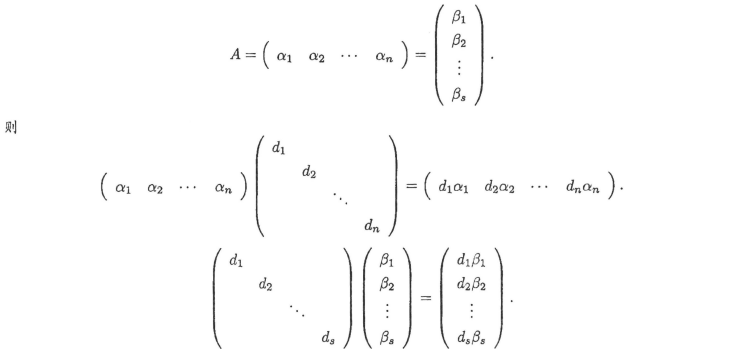
\includegraphics[scale=0.6]{6.png}
	\end{figure}
	
	即$A$右乘对角矩阵$\textup{diag}(d_1,d_2,\dots,d_n)$相当于给$A$的第$i$列元素都乘以$d_i$,
	$A$左乘对角矩阵$\textup{diag}(d_1,d_2,\dots,d_n)$相当于给$A$的第$i$行元素都乘以$d_i$。
\end{theorem}
\begin{theorem}
	(请自行完成以下内容的补充)

	对角矩阵以及准对角矩阵的三则运算、可逆性以及逆运算、乘方运算等规则。
\end{theorem}

\subsubsection{上(下)三角矩阵}
\begin{theorem}
	已知$A$,$B$都是上三角矩阵,且设$A$的主对角元素分别为$a_{11},\dots,a_{nn}$,B的主对角元素分别为
	$b_{11},\dots,b_{nn}$,则
	
	\textup{(1)}$A^{\mathrm{T}}$,$B^\mathrm{T}$都是下三角矩阵;
	
	\textup{(2)}$AB$仍然是上三角矩阵,且$AB$的主对角元素为$a_{11}b_{11},\dots,a_{nn}b_{nn}$;
	
	\textup{(3)}$A$可逆的充要条件是其主对角元均不为$0$,且$A$可逆时,$A^{-1}$也是上三角矩阵,并且$A^{-1}$的主对角元素分别为$a_{11}^{-1},\dots,a_{nn}^{-1}$.
\end{theorem}

\begin{example}
	已知$A_1,\dots,A_n$是$n$个对角元都为$0$的上三角矩阵,证明:$A_1A_2\dots A_n=O$.
\end{example}

\subsubsection{基本矩阵}
只有一个元素为1,其余元素全为0的矩阵称为基本矩阵,第$i$行第$j$列元素为1的基本矩阵记为$E_{ij}$,
他们具有如下性质(可以回忆左右乘对应行列变换):
\begin{theorem}

	\textup{(1)}$AE_{ij}$的结果就是把$A$的第$i$列移到第$j$列的位置,其余元素都为$0$的矩阵;
	
	\textup{(2)}$E_{ij}B$的结果就是把$B$的第$j$行移到第$i$行的位置,其余元素都为$0$的矩阵;
	
	\textup{(3)}$E_{ik}E_{kj}=E_{ij}$,当$k \neq l$时,有$E_{ik}E_{lj}=O$.
\end{theorem}

\subsubsection{其他矩阵}
其他矩阵如正交矩阵、置换矩阵、幂等矩阵、幂零矩阵等,有的会在稍后介绍部分性质,有的
则会在课程进行中或者后续课程中再见到它们。

\subsection{逆矩阵的求解(进阶方法)}
\subsubsection{给定多项式求逆矩阵}
此类题目相信大家已经有所见识,实际上就是通过一些初中所学的因式分解等基本变换得到需要求逆的矩阵与另一个矩阵相乘
可以得到单位矩阵(的一个倍数)。
\begin{example}
	设$A$为非零矩阵,且$A^3=O$,证明:$E+A$和$E-A$都可逆.
\end{example}

\begin{example}
	若$X$,$Y$是两个列向量,且$X^\mathrm{T}Y=2$,证明:

	\textup{(1)}$(XY^\mathrm{T})^k=2^{k-1}(XY^{\mathrm{T}})$;

	\textup{(2)}如果$A=E+XY^\mathrm{T}$,则$A$可逆,并求其逆矩阵.

\end{example}

\subsubsection{利用分块矩阵初等变换*}
我们在前面已经讲解过了打洞法的基础题型,这里再给出一些例子:
\begin{example}
	设$A$、$B$为$n$阶矩阵,证明:若$E\pm AB$可逆,则$E\pm BA$可逆.
\end{example}
\begin{example}
	设$A$为$n$阶矩阵,$B$、$C$分别为$n \times m$、$m \times n$阶矩阵,
	证明:$E_m+CA^{-1}B$可逆$\iff A+BC$可逆.
\end{example}

\subsubsection{求逆的分式思想*}
虽然矩阵没有除法运算,但是我们如果将$(E-A)^{-1}$写成$\frac{E}{E-A}$,再类比泰勒展开
$$\frac{1}{1-x}=1+\sum_{n=1}^\infty x^n(x\in (-1,1))$$我们可以得到(不严谨!只能用来解题的时候当作初步的思路!)
$$(E-A)^{-1}=\frac{E}{E-A}=E+A+A^2+\dots$$

\begin{example}
	已知方阵$A$满足$A^k=O$,其中$k$是一个正整数,求$E-A$的逆.
\end{example}

\begin{example}
	设$A$,$B$分别是$n \times m$和$m \times n$的矩阵,且$E_n \pm AB$可逆,则$E_m \pm BA$可逆.
\end{example}
不难发现这一例是前述4.3.1节中最后一个例题的推广。

\subsubsection{提逆思想*}
这一思想的来源是矩阵逆没有加减相关的运算法则,因此我们需要提逆产生一些乘积项来解决问题。
\begin{example}
	设$A$是$n$阶方阵,且$E-A$,$E+A$和$A$都可逆,证明:$(E-A^{-1})^{-1}+(E-A)^{-1}=E$.
\end{example}

\subsection{矩阵的迹*}
\subsubsection{基本概念与性质}
\begin{definition}
	一个方阵$A$的所有主对角元素之和称为$A$的迹,记为$\textup{tr}(A)$.
\end{definition}
迹的常见性质如下:
\begin{theorem}
	已知$A$,$B$是两个$n$阶矩阵,$k$是一个常数,则

	\textup{(1)}\textup{tr}$(kA)$=$k$\textup{tr}$(A)$;

	\textup{(2)}\textup{tr}$(A+B)$=\textup{tr}$(A)+$\textup{tr}$(B)$;
	
	\textup{(3)}\textup{tr}$(AB)$=\textup{tr}$(BA)$;
	
	\textup{(4)}如果$A$是实矩阵,则$A=O \iff$\textup{tr}$(A^{\mathrm{T}}A)=0$.
\end{theorem}

我们先来看一个基本的例子练习一下:
\begin{example}
	证明:不存在方阵$A$、$B$使得$AB-BA=E$.
\end{example}

接下来我们介绍一个性质,这一性质的证明需要利用矩阵的秩中讲到的一些技巧:
\begin{theorem}
	已知 $n$ 阶矩阵 $A$ 的秩为 $1$ ,证明:$A^k=\textup{tr}(A)^{k-1}A$.
\end{theorem}
这一定理的证明需要用到矩阵的分解,在2020年吴志祥老师班期中考试有出现,可以参考
辅学网站上的解答。

当然我们还会在特征值一章再次见到矩阵的迹,相关内容在最后一个专题会展开讲述。

\subsubsection{幂零矩阵}
幂零矩阵是一种特殊的矩阵,幂零矩阵$A$存在一个正整数$k$使得$A^k=O$,
它具有如下性质(部分需要用到特征值,所以最后一个专题还会提及):
\begin{theorem}
	若$n$阶矩阵$A$为幂零矩阵,则

	\textup{(1)}$A^n=O$;

	\textup{(2)}$A\pm E$均为可逆矩阵;

	\textup{(3)}幂零矩阵对应的线性变换一定存在一个矩阵表示使得矩阵为上三角矩阵且对角线元素全为\textup{0};
	
	\textup{(4)}$A$为幂零矩阵$\iff \forall k \in N^+$,\textup{tr}$(A^k)$=\textup{0}.
\end{theorem}

\begin{example}
	若$A$、$B$为两个$n$阶矩阵且满足$AB-BA=A$,证明:

	\textup{(1)}$A$不可逆;

	\textup{(2)}$A$是幂零矩阵.
\end{example}

\subsection{矩阵的幂}
\begin{enumerate}
	\item 找规律
	
	在矩阵的转置中我们已经见识了一种找规律的方式,下面是一种类似的题型:
	\begin{example}
		计算$(PAQ)^k$,其中
		$$P=\begin{pmatrix}2 & 3 \\ 1 & 2\end{pmatrix}, A=\begin{pmatrix}2 & 0 \\ 0 & -1\end{pmatrix}, Q=\begin{pmatrix}2 & -3 \\ -1 & 2\end{pmatrix}$$
	\end{example}
	
	\begin{example}
		设$A=\begin{pmatrix}0 & -1 & 0 \\ 1 & 0 & 0 \\ 0 & 0 & -1 \end{pmatrix}$,
		$P^{-1}AP=B$,求$B^{2004}-2A^2$.
	\end{example}

	还有一种找规律基于幂等矩阵,显然幂等矩阵的任意次方都与其平方相等是很好的性质,另一种找规律基于对合矩阵,即平方等于单位矩阵的矩阵,我们这里
	主要与大家分享关于幂零矩阵的方法,例子如下:
	\begin{example}
		求$A=\begin{pmatrix}a & 1 & 0 & 0 \\ 0 & a & 1 & 0 \\ 0 & 0 & a & 0 \\ 0 & 0 & 0 & a \end{pmatrix}^n$.
	\end{example}
	在上例中,我们采用将矩阵分为$A=tE+B$的方法,会发现矩阵$B$为上三角矩阵且对角线上全为0,是典型的幂零矩阵,利用这一性质可以快速解题。
	\item 数学归纳法
	\begin{example}
		求$A=\begin{pmatrix}\cos\alpha & \sin\alpha \\ -\sin\alpha & \cos\alpha\end{pmatrix}^n$.
	\end{example}
	这一问题对应我们常见的旋转变换。
	\begin{example}
		证明$\begin{pmatrix}
			a & c \\ 0 & b
		\end{pmatrix}^n=\begin{pmatrix}
			a^n & (a^{n-1}+a^{n-2}b+\dots+b^{n-1})c \\ 0 & b^n
		\end{pmatrix}$.
	\end{example}
	\item 利用秩为1的矩阵
	
	在我们有关秩的讨论中已经提到了如果$A$是秩为1的矩阵,那么$A^n=(\textup{tr}(A))^{n-1}A$,我们可以利用这一性质解决问题。
	\begin{example}
		已知$M$是秩为$1$的矩阵,记\textup{tr}$(M)=b$,讨论$(aE+M)^n$的计算结果.
	\end{example}

	\begin{example}
		已知$A$是数域$P$上的一个$2$阶方阵,且存在正整数$l$使得$A^l=O$,证明:$A^2=O$.
	\end{example}
	事实上,我们在幂零矩阵的讨论中已经提及了上例的一般情况。

	\begin{example}
		已知数列$\{a_n\}$,$\{b_n\}$满足$a_0=-1$,$b_0=3$,且
		$$\begin{cases}
			a_n=3a_{n-1}+b_{n-1}+2^{n-1} \\ b_n=2a_{n-1}+4b_{n-1}+2^n
		\end{cases}$$
		求$\{a_n\}$,$\{b_n\}$的通项公式.
	\end{example}
	\item 利用初等矩阵的性质
	\begin{example}
		设$A$为三阶矩阵,$P$为三阶可逆矩阵,$P^{-1}AP=B$,其中$P=\begin{pmatrix}
			0 & 2 & -1 \\ 1 & 1 & 2 \\ -1 & -1 & -1
		\end{pmatrix}$,$B=\begin{pmatrix}
			0 & 0 & -1 \\ 0 & -1 & 0 \\ -1 & 0 & 0
		\end{pmatrix}$,求$A^{2022}$.
	\end{example}

	\item 利用对角化
	
	若一个矩阵$A$可对角化,即存在可逆矩阵$P$使得$A=P^{-1}\Lambda P$(其中$\Lambda$为对角矩阵),
	在这种形式下$A$的幂是很好求的。
	\begin{example}
		已知$A=\begin{pmatrix}
			0 & \cfrac{1}{2} & \cfrac{1}{2} \\ 1 & -\cfrac{1}{2} & \cfrac{1}{2} \\ 1 & -\cfrac{1}{2} & \cfrac{1}{2}
		\end{pmatrix}$,求$A^n$.
	\end{example}

\end{enumerate}

\section{矩阵的秩的定义与性质}
本节内容理解难度较大,事实上这里利用了很多线性空间与线性映射的思想,
也有很多技巧性的内容,因此希望各位同学根据自己实际情况理解掌握。虽然很推荐
这部分内容采用与教材不同的思路去理解,更多利用线性空间与线性映射的抽象知识思考,但是如果
理解起来有一定困难也记住一些结论去解决一些问题。

还有一部分应当属于本节的内容将在专题五线性方程组的部分提及,因此本节不再专门
讲解利用线性方程组的思想解决矩阵的秩相关问题的部分。

\subsection{矩阵的三个秩的基本概念与性质}
我们首先给出矩阵的三个秩的定义:
\begin{definition}
	设$A$是线性映射$\sigma$对应的矩阵,我们把$\sigma$的秩也称为矩阵$A$的秩,
	记为$r(A)$.我们将矩阵$A$的所有行向量组成的秩称为$A$的行秩,
	所有列向量组成的向量组的秩称为$A$的列秩.
\end{definition}
对于以上三个秩我们有重要的定理如下:
\begin{theorem}
	任意矩阵的秩 = 行秩 = 列秩.
\end{theorem}
这一定理的证明,矩阵的秩 = 列秩的部分根据线性映射的相关概念是显然的,行秩的部分
教材中有较为繁琐的证明,在本讲义下面的内容会有更加形象的解释。

实际上,这一定理有两个重要的直接推论,一是将求矩阵的秩的问题转化为求矩阵行/列极大线性无关向量组的问题,
第二是矩阵的秩等于其转置的秩。

可能很多同学对于行秩、列秩相等以及转置的几何意义很感兴趣。实际上我们有两种获得转置矩阵的
方式,第一种来源于我们之前讨论的对偶空间上的线性映射对应的矩阵,这种方式可能不够直观。
另一种获得的方法基于内积,感兴趣的同学可以了解矩阵的伴随(不是行列式中的伴随矩阵)。

我们可以研究矩阵及其转置的关系,我们可以用一个图形来表示:
\begin{figure}[h]
	\centering
	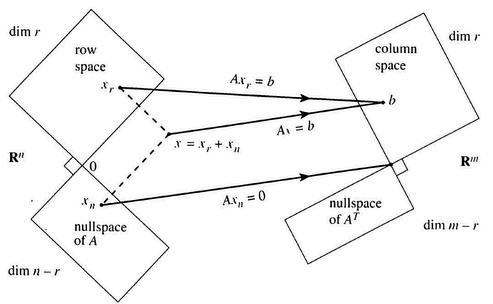
\includegraphics[scale=0.5]{5.png}
\end{figure}

我们观察到以下几点:
\begin{enumerate}
	\item 矩阵的行空间与解空间(零空间)互为正交补(直观理解两个空间就是互相垂直且互为补空间),这一点应当是在正交的内容中有所提及的;
	\item 矩阵的列空间与其转置矩阵的零空间互为正交补,这一点实际与上一条等价.
\end{enumerate}

接下来我们来看行秩(列秩比较显然,此处不再详细展开)。我们首先得到解空间的维数,这可以直接
根据维数公式得到:$\dim N(A)=n-r(A)$,根据正交补的性质,我们的可以得到行秩即为
$n-(n-r(A))=r(A)$.于是我们得到了一个基于正交补的行秩解释.

\subsection{相抵标准形}
此处我们需要首先回顾一个基本定理:
\begin{theorem}
	初等变换不改变矩阵的秩(包括行变换和列变换).
\end{theorem}
由这一定理我们可以推导出相抵标准形:
\begin{theorem}
	若$r(A_{m \times n})=r$,则存在可逆矩阵$P$和$Q$,使得
	$$PAQ=\begin{pmatrix}
		E_r & 0 \\ 0 & 0
	\end{pmatrix}=U_r,$$
	其中$E_r$表示$r$阶单位矩阵.
\end{theorem}
这一定理证明直接使用定理4以及可逆矩阵可以拆分为初等矩阵的乘积即可。
其中$U_r$称为相抵标准形。我们称两个矩阵相抵即两个矩阵可以通过一系列
初等变换可以互相转化。由此我们得到关于矩阵相抵的两个等价命题:

1. 矩阵$A$与$B$相抵$\iff$存在可逆矩阵$P$和$Q$使得$PAQ=B$;

2. 矩阵$A$与$B$相抵$\iff r(A)=r(B)$.

\begin{example}
	设$A=\begin{pmatrix}
		1 & 0 & 2 & -4 \\ 2 & 1 & 3 & -6 \\ -1 & -1 & -1 & 2
	\end{pmatrix}$, 求

	\textup{(1)}$A$的秩$r$和相抵标准形;

	\textup{(2)}$3$阶可逆矩阵$P$和$4$阶可逆矩阵$Q$使得$PAQ=\begin{pmatrix}
		E_r & 0 \\ 0 & 0
	\end{pmatrix}$.
\end{example}

关于相抵标准形,我们需要在此补充一个常用的技术,即相抵标准形的分解:

我们对$s \times n$矩阵$\begin{pmatrix}
	E_r & O \\ O & O
\end{pmatrix}$有一种很重要的分解:
$$\begin{pmatrix}
	E_r & O \\ O & O
\end{pmatrix}=\begin{pmatrix}
	E_r \\ O
\end{pmatrix}\begin{pmatrix}
	E_r & O
\end{pmatrix}$$ 由此我们可以知道任意一个非零矩阵都可以被分解成一个列满秩矩阵和一个
行满秩矩阵的乘积:

$$A=P\begin{pmatrix}
	E_r & O \\ O & O
\end{pmatrix}Q=P\begin{pmatrix}
	E_r \\ O
\end{pmatrix}\begin{pmatrix}
	E_r & O
\end{pmatrix}Q$$
记$P_1=P\begin{pmatrix}
	E_r \\ O
\end{pmatrix}$,$Q_1=\begin{pmatrix}
	E_r & O
\end{pmatrix}Q$,则$A=P_1Q_1$,且$P_1$和$Q_1$分别为列满秩、行满秩矩阵。

我们可以利用相抵标准形解决很多问题,例如下一节中部分秩不等式的证明:
\begin{example}
	\textup{(1)}$r\begin{pmatrix}
		A & O \\ O & B
	\end{pmatrix}=r(A)+r(B)$.

	\textup{(2)}$r\begin{pmatrix}
		A & D \\ O & B
	\end{pmatrix}\ge r(A)+r(B)$,
	$r\begin{pmatrix}
		A & O \\ C & B
	\end{pmatrix}\ge r(A)+r(B)$.
\end{example}

\subsection{秩相关的等式与不等式}
本节的内容实际上部分内容有一定的技巧性,对于荣誉课程来说还是以理解为主(所以
其实本节中提到的很多内容都只是介绍性的,而非要求大家熟练掌握,但是遇见了要有
一些基本的思路而不能完全不理解),可能下面列出定理的时候显得比较繁冗,但是实
际上我们更重视其中的理解而非硬套结论。

我们首先给出一些常见的秩相关的不等式或等式,这些式子希望各位同学能够理解其含义,
而非机械记忆套用。下面这些等式/不等式的证明方式非常多,实际上可以利用之前所说化为
相抵标准形的方法,也可以利用线性相关性的方法,也可以回到线性映射进行考量。总之
解决的方法非常多,希望各位同学能熟练推导理解。
\begin{enumerate}
	\item $r(A)=r(PA)=r(AQ)=r(PAQ)$,其中$P$、$Q$可逆
	\item $|r(A)-r(B)|\le r(A\pm B) \le r(A)+r(B)$
	\item $r(AB) \le \min\{r(A),\ r(B)\}$
	\item $r(A)=r(A^\mathrm{T})=r(AA^\mathrm{T})=r(A^\mathrm{T}A)$(注意第二个等号需要实矩阵作为前提条件)
	\item $A \in \mathbf{F}^{s \times n}$,$B \in \mathbf{F}^{n \times m}$,
	则$r(AB) \ge r(A)+r(B)-n$.(可以视为结论6的推论,特例$AB=O$时有$r(A)+r(B)\le n$)
	\item $r(ABC) \ge r(AB)+r(BC)-r(B)$.(还可以考虑A,B,C相等的特殊情况的结果)
\end{enumerate}

分块矩阵的相关公式在上一小节的例题中已经书写过,此处不再重复。

一般而言,解决较为复杂的秩的问题时,我们可以采用如下方法:

(1)利用(分块)矩阵初等变换;

(2)利用线性方程组解的一般理论(将在专题五讲解);

(3)利用向量组线性相关性;

(4)利用已知的矩阵秩的等式和不等式。实际上等式很多时候基于可逆矩阵变换或者两个不等号夹逼。

相关方法的应用都在本节最后的习题中有所体现,当然首要的任务是掌握上述基本的秩不等式的证明,
很多也利用了上面的思想,并且解法不唯一。

\subsection{习题}
\centerline{\heiti A组}
\begin{enumerate}
	\item 证明:矩阵添加一列(或一行),其秩或不变,或增加1.
	\item 设$A$是$s \times n$矩阵,$B$是$A$前$m$行构成的$m \times n$矩阵,证明:
	$r(B) \ge r(A) + m - s$.
	\item 若$A$、$B$为两个$n$阶矩阵,则

	$\textup{A}.\ r(A\ B)=r(A^\mathrm{T}\ B^\mathrm{T})$

	$\textup{B}.\ r(A\ AB)=r(A)$

	$\textup{C}.\ r(A\ B)=\max\{r(A),\ r(B)\}$

	$\textup{D}.\ r(A\ BA)=r(A)$
	\item 若$A$、$B$为两个$n$阶矩阵且满足$A+B=AB$,证明:

	(1)$A-E$和$B-E$均可逆;

	(2)$AB=BA$;

	(3)$r(A)=r(B)$.
\end{enumerate}
\centerline{\heiti B组}
\begin{enumerate}
	\item 设$A$为$n$阶矩阵,且$r(A) < n$,又$A_{11} \neq 0$,证明:存在常数$k$,使得
	$(A^*)^2=kA^*$.
	\item (利用相抵标准形)证明以下结论:
	
	(1)设$B_1$,$B_2$为$s \times n$列满秩矩阵,证明:存在$s$阶可逆矩阵
	$C$使得$B_2=CB_1$.

	(2)设$B_1$,$B_2$为$s \times n$行满秩矩阵,证明:存在$n$阶可逆矩阵
	$C$使得$B_2=B_1C$.
	
	(3)任意秩为$r$的矩阵都可以被分解为$r$个秩为$1$的矩阵之和.

	(4)已知$A$是$n$阶方阵,证明:存在$n$阶方阵$B$使得$A=ABA$,$B=BAB$.
	\item 设$B$是$3 \times 1$矩阵,$C$是$1 \times 3$矩阵,证明:$r(BC) \le 1$.
	反之,若$A$是秩为1的$3 \times 3$矩阵,证明:存在$3 \times 1$矩阵$B$和$1 \times 3$矩阵$C$,使得$A = BC$.
	\item 设$\alpha$、$\beta$为$n$维列向量,且$A=\alpha\alpha^\mathrm{T}+\beta\beta^\mathrm{T}$.
	
	(1)证明:$r(A) \le 2$;

	(2)若$\alpha$、$\beta$线性相关,证明:$r(A) \le 1$.
	\item 设 $A \in M_{m \times n}(\mathbf{F})$,$r(A)=r$,$k$ 是满足条件 $r \leq k \leq n$ 的任意整数,证明存在 $n$ 阶方阵 $B$,使得 $AB=O$,且 $r(A)+r(B)=k$.
	\item 设$A$是$m \times n$矩阵($m \le n$),$r(A)=m$,证明:存在$n \times m$矩阵$B$使得$AB=E$.
	\item 设$A,\ B \in M_n(\mathbf{F})$,$r(A)+r(B) \le n$,证明:存在可逆矩阵$M$,使得$AMB=O$.
\end{enumerate}

\centerline{\heiti C组}
\begin{enumerate}
	\item (打洞法)已知$A$是一个$s \times n$矩阵,证明:$r(E_n-A^\mathrm{T}A)-r(E_s-AA^\mathrm{T})=n-s$.
	\item 利用打洞法完成以下两个问题((2)也可以不使用打洞法,可以思考其他方式解决):
	
	(1)设$n$阶方阵$A$,$B$,$C$,$D$满足$AC+BD=E$,证明:$r(AB) = r(A)+r(B)-n$.
	
	(2)$n$阶方阵$A$,$B$满足$AB=BA$,证明:$r(AB)+r(A+B)\le r(A)+r(B)$.
	\item $f(x)=f_1(x)f_2(x)$是多项式,且$f_1(x)$与$f_2(x)$互素,则$f(A)=O$的充要条件是$r(f_1(A))+r(f_2(A))=n$.
	(注:此题的推论非常多,如$A^2=A$,$A^n=E$等形式的结论都可以利用这个例子推导出)
	\item 设$A$、$B$分别为$3 \times 2$和$2 \times 3$实矩阵,若$AB=\begin{pmatrix}
		8 & 0 & -4 \\ -\cfrac{3}{2} & 9 & -6 \\ -2 & 0 & 1
	\end{pmatrix}$,求$BA$.
\end{enumerate}

\chapter{行列式}

\section{Overview}
\begin{figure}[h]
	\centering
	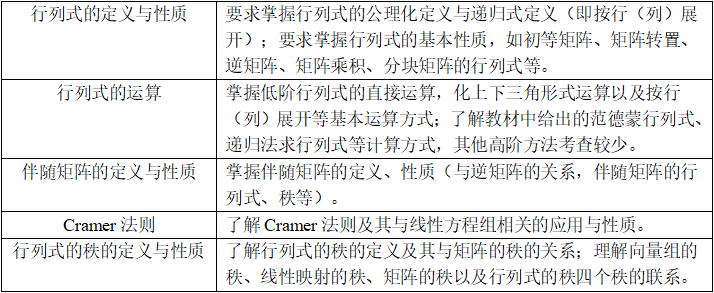
\includegraphics[scale=0.58]{7.png}
\end{figure}

\section{行列式的定义与性质}
很多教材采用“逆序数”定义行列式(感兴趣的同学可以参考丘维声《高等代数》等教材),但是本教材未提及,因此
我们作为复习课也不展开描述。本教材使用公理化定义(使用一些规则描述)并讲解了
递归式定义(按行(列)展开)。

\subsection{公理化定义}
\begin{definition}
	数域$\mathbf{F}$上的一个$n$阶行列式是取值于$\mathbf{F}$的$n$个$n$维向量
	$\alpha_1,\alpha_2,\dots,\alpha_n \in \mathbf{F}^n$的一个函数,且$\forall \alpha_i,\beta_i \in \mathbf{F}^n$
	和$\forall \lambda \in \mathbf{F}$,满足下列规则:
	
	\textup{1}.(齐性)$D(\alpha_1,\dots,\lambda\alpha_i,\dots,\alpha_n)=\lambda D(\alpha_1,\dots,\alpha_i,\dots,\alpha_n)$\textup{;}

	\textup{2}.(加性,与\textup{1}合称线性性)
	
	$D(\alpha_1,\dots,\alpha_i+\beta_i,\dots,\alpha_n)=D(\alpha_1,\dots,\alpha_i,\dots,\alpha_n)+D(\alpha_1,\dots,\beta_i,\dots,\alpha_n)$\textup{;}

	\textup{3}.(反对称性)$D(\alpha_1,\dots,\alpha_i,\dots,\alpha_j,\dots,\alpha_n)=-D(\alpha_1,\dots,\alpha_j,\dots,\alpha_i,\dots,\alpha_n)$\textup{;}

	\textup{4}.(规范性)$D(e_1,e_2,\dots,e_n)=1$.
\end{definition}
在公理化定义中,我们将行列式定义为一个满足特定的运算性质的从列向量组合到数的函数。
事实上,公理化定义从是逆序数定义可以推导出的行列式的运算性质,教材采用这种定义避开了繁琐的说明。
除此之外,我们不难看出公理化定义可以形象地理解为对$n$维空间中体积的定义,
对几何意义感兴趣的同学可以参考3b1b《线性代数的本质》系列视频相关内容。
\begin{example}
	使用定义$1$验证下述命题的正确性:

	\textup{1}. 若行列式有一列为零向量,则行列式的值等于$0$.

	\textup{2}. 若行列式有两列元素相同,则行列式的值等于$0$.

	\textup{3}. 若行列式有两列元素成比例,则行列式的值等于$0$.

	\textup{4}. 对行列式做倍加列变换,行列式的值不变.

	\textup{5}. 若$\alpha_1,\alpha_2,\dots,\alpha_n$线性相关,则$D(\alpha_1,\alpha_2,\dots,\alpha_n)=0$.
\end{example}

\begin{example}
	设向量$\alpha_1$,$\alpha_2$,$\beta_1$,$\beta_2$为三维列向量,又$A=(\alpha_1,\alpha_2,\beta_1)$,$B=(\alpha_1,\alpha_2,\beta_2)$,
	且$|A|=3$,$|B|=2$,求$|2A+3B|$.
\end{example}

\subsection{递归式定义}
首先需要回顾余子式和代数余子式的概念:
\begin{definition}
	在$n$阶行列式$D=|a_{ij}|_{n \times n}$中,去掉元素$a_{ij}$所在的第$i$行和第$j$列的所有元素
	而得到的$n-1$阶行列式称为元素$a_{ij}$的余子式,记作$M_{ij}$,并把数$A_{ij}=(-1)^{i+j}M_{ij}$
	称为元素$a_{ij}$的代数余子式.
\end{definition}
注意,虽然余子式和代数余子式在名称中含有式,但实际上他们是一个值。实际上行列式也称为“式”,但这些“式”
只是形状上有个形式,实际上只是一个值。
\begin{example}
	根据定义$2$计算行列式$\begin{vmatrix}
		2 & 1 & 3 \\
		-1 & 0 & 2 \\
		1 & 5 & -2
	\end{vmatrix}$每个元素的余子式和代数余子式.
\end{example}

接下来我们便可以给出递归式定义:
\begin{definition}
	设$D=|a_{ij}|_{n \times n}$,则
	\begin{equation}
		D=\sum_{k=1}^{n}a_{kj}A_{kj}=a_{1j}A_{1j}+a_{2j}A_{2j}+\dots+a_{nj}A_{nj},\ j=1,2,\dots,n
	\end{equation}
	\begin{equation}
		D=\sum_{k=1}^{n}a_{ik}A_{ik}=a_{i1}A_{i1}+a_{i2}A_{i2}+\dots+a_{in}A_{in},\ i=1,2,\dots,n
	\end{equation}
\end{definition}
其中$A_{ij}$即为定义2给出的代数余子式,(1)式称为$D$对第$j$列的展开式,(2)式称为$D$对第$i$行的展开式。这一定义与公理化定义的
等价性不难证明。事实上,这一定义被称为递归式定义的原因是显然的(如果在程序设计课程中已经学习过递归的概念),它使用$n-1$阶行列式定义$n$阶行列式,我们对任意$n$阶行列式
都可以递归展开到1阶,从而得到最终行列式计算结果。
\begin{example}
	利用定义$3$计算例$3$中的行列式,可以行列展开均使用并在上述公式中选取不同$i$和$j$以熟悉定义$3$,并注意体会递归式定义的含义.
\end{example}

递归式定义有一个相关的结论如下:
\begin{theorem}
	$n$阶行列式$D=|a_{ij}|_{n \times n}$的某一行(列)元素与另一行(列)相应元素的代数余子式
	的乘积之和等于$0$,即
	\begin{equation}
		\sum_{k=1}^{n}a_{kj}A_{ki}=a_{1j}A_{1i}+a_{2j}A_{2i}+\dots+a_{nj}A_{ni}=0,\ j \neq i
	\end{equation}
	\begin{equation}
		\sum_{k=1}^{n}a_{jk}A_{ik}=a_{j1}A_{i1}+a_{j2}A_{i2}+\dots+a_{jn}A_{in}=0,\ j \neq i
	\end{equation}
\end{theorem}
我们若将行列式第$j$列元素替换为第$i$列元素,那么上述(3)式根据定义3就是在求替换后的行列式,
并且有两列元素相同的行列式为0,我们便可以轻松地证明(3),实际上(4)同理也可证明。同学们可能
对(1)-(4)式繁杂的下标感到陌生,因此安排了例2-4希望大家熟悉这些公式.
\begin{example}
	对例$3$中的矩阵验证定理$1$的正确性.
\end{example}
这一节中行列式是按照一行(列)展开的,若按多行(列)展开则需要相应的拉普拉斯定理,感兴趣的同学可以了解。
\subsection{行列式的常用性质}
设$A,B \in \mathbf{F}^{n \times n}$,$k \in \mathbf{F}$,则

1. 一般情况下,$|A \pm B| \neq |A|\pm|B|$;

2. $|kA|=k^n|A|$;

3. $A$可逆$\iff |A| \neq 0$;

4. 初等矩阵行列式(注意初等矩阵不分行列,左乘右乘区分初等行列变换):$|E_{ij}|=-1$,$|E_i(c)|=c$,$|E_{ij}(k)|=1$;

5. 利用4中的结论可以得到$|A^\mathrm{T}|=|A|$:

6. 利用4中的结论可以得到$|AB|=|A||B|$,$|A^k|=|A|^k$;

7. 利用4中的结论(求出初等矩阵逆矩阵行列式)可以得到若$A$可逆,则$|A^{-1}|=|A|^{-1}$.

以上性质都可以基于定义或上述其他性质得到,下面介绍的性质需要用到“打洞法”(分块矩阵初等变换)
来证明:

1. $\begin{vmatrix}
	A & O \\ O & B
\end{vmatrix} = \begin{vmatrix}
	A & O \\ C & B
\end{vmatrix} = \begin{vmatrix}
	A & D \\ O & B
\end{vmatrix} = |A||B|,\ \begin{vmatrix}
	O & A \\ B & C
\end{vmatrix} = (-1)^{kr}|A||B|$;

2. 当$A$可逆时,有$\begin{vmatrix}
	A & B \\ C & D
\end{vmatrix} = |A||D-CA^{-1}B|$,当$D$可逆时,有
$\begin{vmatrix}
	A & B \\ C & D
\end{vmatrix} = |D||A-BD^{-1}C|$,当$B$可逆时,有
$\begin{vmatrix}
	A & B \\ C & D
\end{vmatrix} = (-1)^{mn}|B||C-DB^{-1}A|$,当$C$可逆时,有
$\begin{vmatrix}
	A & B \\ C & D
\end{vmatrix} = (-1)^{mn}|C||B-AC^{-1}D|$;

3. 设$A$和$B$分别是$n \times m$和$m \times n$矩阵,则$|E_n \pm AB|=|E_m \pm BA|$,且
$|\lambda E_n \pm AB|=\lambda^{n-m}|\lambda E_m \pm BA|(n \ge m)$.

还有一部分由这些性质可以推导的其他性质将出现在C组习题中供参考。这部分主要是技巧性内容,可以选择性完成。
\subsection{习题}
\centerline{\heiti A组}
\begin{enumerate}
	\item 设$\alpha_1,\alpha_2,\alpha_3$为三维列向量,令$A=(\alpha_1,\alpha_2,\alpha_3)$,
	且$|A|=2$,求$|\alpha_1+\alpha_2+\alpha_3,\alpha_1+3\alpha_2+9\alpha_3,\alpha_1+4\alpha_2+16\alpha_3|$.
	\item 求证以下命题:
	
	(1)奇数阶反对称矩阵不可逆;
	
	(2)若$A$是$n$阶可逆对称矩阵,$B$是$n$阶反对称矩阵,则当$n$为奇数时,齐次线性方程组$(AB)X=O$有非零解.
\end{enumerate}

\centerline{\heiti B组}
\begin{enumerate}
	\item 设$D=\begin{vmatrix}
		3 & 0 & 4 & 1 \\ 2 & 3 & 1 & 4 \\ 0 & -7 & 8 & 3 \\ 5 & 3 & -2 & 2
	\end{vmatrix}$,求

	(1)$A_{21}+A_{22}+A_{23}+A_{24}$;

	(2)$A_{31}+A_{33}$;

	(3)$M_{41}+M_{42}+M_{43}+M_{44}$;
	\item 求参数 $a,\ b$  的值,使得 $\begin{vmatrix}1 & 1 & 1 \\ x & y & z \\u & v & w\end{vmatrix}=1,\ \begin{vmatrix}1 & 2 & -5 \\ x & y & z \\u & v & w\end{vmatrix}=2,\ \begin{vmatrix}2 & 3 & b \\ x & y & z \\u & v & w\end{vmatrix}=a$ 都成立,并求$\begin{vmatrix}x & y & z \\ 1 & -1 & 5 \\u & v & w\end{vmatrix}$.
	\item 设$A$,$B$为三阶矩阵,且$|A|=3$,$|B|=2$,且$|A^{-1}+B|=2$,求$|A+B^{-1}|$.
	\item 设$A$为$n$阶正交矩阵,即$AA^\mathrm{T}=A^\mathrm{T}A=E$,且$|A|<0$,证明:$|E+A|=0$.
	\item 已知齐次线性方程组$$\begin{cases}
		a_{11}x_1+a_{12}x_2+\cdots+a_{1n}x_n=0 \\
		a_{21}x_1+a_{22}x_2+\cdots+a_{2n}x_n=0 \\
		\cdots \\
		a_{n-1,1}x_1+a_{n-1,2}x_2+\cdots+a_{n-1,n}x_n=0
	\end{cases},$$设$M_j(j=1,2,\cdots,n)$表示$A$划掉第$j$列所得的$n-1$阶子式,证明:

	(1)$(M_1,-M_2,\cdots,(-1)^{n-1}M_n)$是方程组的一个解;

	(2)若$r(A)=n-1$,则方程组的解全是$(M_1,-M_2,\cdots,(-1)^{n-1}M_n)$的倍数.
\end{enumerate}

\centerline{\heiti C组}
\begin{enumerate}
	\item 设$A$,$B$,$C$,$D$均为$n$阶方阵,且$AC=CA$,证明:
	$$\begin{vmatrix}
		A & B \\ C & D
	\end{vmatrix} = |AD-CB|.$$

	\item 设$A$为$n$阶可逆矩阵,$\alpha$,$\beta$为$n$维列向量,证明:
	$$|A+\alpha\beta^{\mathrm{T}}|=|A|(1+\beta^\mathrm{T}A^{-1}\alpha).$$
	\item 设$A$,$B$均为$n$阶方阵,证明:
	$$\begin{vmatrix}
		A & B \\ B & A
	\end{vmatrix} = |A+B||A-B|.$$
	\item 设$A$,$B$,$C$,$D$均为$n$阶方阵,且$r\begin{pmatrix}
		A & B \\ C & D
	\end{pmatrix}=n$,证明:
	$$\begin{vmatrix}
		|A| & |B| \\ |C| & |D|
	\end{vmatrix} = 0.$$
	\item $^*$(对角占优)设$A=(a_{ij})_{n \times n}$是一个$n$级矩阵,证明:
	
	(1)若$A$为复矩阵,且$|a_{ii}|>\sum_{j \neq i}|a_{ij}|$,那么$|A|\neq 0$;

	(2)若$A$为实矩阵,且$a_{ii}>\sum_{j \neq i}|a_{ij}|$,那么$|A|>0$;

	(3)(推论)存在充分大的实数$M$,使得$t>M$时,$tE+A$可逆.
\end{enumerate}

\section{行列式的运算}
\subsection{概述}
本节内容按照往年经验不是考试重点,实际上行列式这章在往年单独出现的
频率较低,一般都在求解特征值或者作为判断可逆等情况下作为结论使用,但是我们仍然需要掌握基本的行列式计算方法,
至少教材中给出的例题需要熟悉。

一般而言行列式的计算方法有根据定义求解(包括逆序数定义(包括低阶行列式直接计算公式)、公理化定义和递归式定义(或拉普拉斯定理))、
高斯消元法化为上三角矩阵求解、拆分法(大拆分法、小拆分法)求解、加边法(升阶法)求解、特殊行列式求解
(如“箭形”行列式,循环行列式,范德蒙行列式)、递推法求解、数学归纳法求解(这两种方法一般用于大对角形)、
打洞法求解以及利用特征值求解等,具体方法不在此展开,一般教辅书上都有详细介绍,因为这不是线性代数荣誉课
重点内容,因此我们不详细说明这些方法,只在下面的习题中给出几个例子。

\subsection{习题}
注:本节习题只给出少量练习回顾基本方法以及给出少量特殊的例子,如果需要系统性练习高阶方法的建议参考此前陈小川学长的行列式授课资料
或其他参考书等。

\centerline{\heiti A组}
\begin{enumerate}
	\item 推导二阶行列式与三阶行列式直接计算的一般公式.
	\item 利用行列式的定义计算对角矩阵,副对角矩阵(即只有副对角线元素非0)以及上(下)三角矩阵行列式.
	\item 利用初等变换化对角矩阵的方法求四阶行列式$\begin{vmatrix}
		1 & 2 & -2 & 3 \\ -1 & -2 & 4 & -2 \\ 0 & 1 & 2 & -1 \\ 2 & 3 & -3 & 10
	\end{vmatrix}$.
	\item 计算行列式$\begin{vmatrix}
		\alpha & \beta & \gamma \\
		\gamma & \alpha & \beta \\
		\beta & \gamma & \alpha
	\end{vmatrix}$,其中$\alpha$,$\beta$,$\gamma$是方程$x^3+px+q=0$的三个根.
\end{enumerate}

\centerline{\heiti B组}
\begin{enumerate}
	\item (范德蒙行列式)计算行列式$\begin{vmatrix}
		1 & 1 & 1 &  \cdots & 1 \\
		a_1 & a_2 & a_3 &  \cdots & a_n \\
		a_1^2 & a_2^2 & a_3^2 &  \cdots & a_n^2 \\
	  \vdots & \vdots & \vdots &  & \vdots  \\
		a_1^{n-1} & a_2^{n-1} & a_3^{n-1} & \cdots & a_n^{n-1} 
	  \end{vmatrix}$,并写出范德蒙行列式不为0的条件.
	\item (数学归纳法与递推)证明$\begin{vmatrix}
		\cos\alpha & 1 & 0 &  \cdots & 0 & 0 \\
		1 & 2\cos\alpha & 1 &  \cdots & 0 & 0 \\
		0 & 1 & 2\cos\alpha &  \cdots & 0 & 0 \\
		\vdots & \vdots & \vdots &  & \vdots  \\
		0 & 0 & 0 & \cdots & 2\cos\alpha & 1 \\
		0 & 0 & 0 & \cdots & 1 & 2\cos\alpha 
	\end{vmatrix}=\cos n\alpha$.
	\item 利用升阶法或拆项与递推的方法求解行列式
	$$\begin{vmatrix}
		1+a_1 & 1 & \cdots & 1 \\
		1 & 1+a_2 & \cdots & 1 \\
	  \vdots & \vdots &  & \vdots  \\
		1 & 1 & \cdots & 1+a_n
	  \end{vmatrix}.$$
	\item 利用递推法或三角法或拉普拉斯定理计算行列式
	$$D_{2n}=\begin{vmatrix}
		a &  &  &  &  & b \\
		  & \ddots &  &  & \begin{sideways}$\ddots$\end{sideways} &  \\
		  &  & a & b &  &  &   \\
		  &  & b & a &  &  &   \\  
		  & \begin{sideways}$\ddots$\end{sideways} &  &  & \ddots &  \\
		b &  &  &  &  & a
	\end{vmatrix}.$$
\end{enumerate}

\centerline{\heiti C组}
\begin{enumerate}
	\item 利用上一节中的打洞性质或初等变换或拆分法计算行列式
	$\begin{vmatrix}
		a & b & b &  \cdots & b \\
		b & a & b &  \cdots & b \\
		b & b & a &  \cdots & b \\
	  \vdots & \vdots & \vdots &  & \vdots  \\
		b & b & b & \cdots & a 
	  \end{vmatrix}$.

	\item 利用矩阵分解计算行列式$\begin{vmatrix}
		\sin(\alpha_1+\beta_1) & \sin(\alpha_1+\beta_2) & \cdots & \sin(\alpha_1+\beta_n) \\
		\sin(\alpha_2+\beta_1) & \sin(\alpha_2+\beta_2) & \cdots & \sin(\alpha_2+\beta_n) \\
	  \vdots & \vdots &  & \vdots  \\
	    \sin(\alpha_n+\beta_1) & \sin(\alpha_n+\beta_2) & \cdots & \sin(\alpha_n+\beta_n)
	  \end{vmatrix}$.

	\item (循环行列式)记$a_{ij}=|i-j|$,且$A=(a_{ij})_{n \times n}$,计算$A$的行列式.
	\item (递推法求大对角形行列式)
	
	计算$n$阶行列式$\begin{vmatrix}
		1-a_1 & a_2 & 0 &  \cdots & 0 & 0 \\
		-1 & 1-a_2 & a_3 &  \cdots & 0 & 0 \\
		0 & -1 & 1-a_3 &  \cdots & 0 & 0 \\
		\vdots & \vdots & \vdots &  & \vdots  \\
		0 & 0 & 0 & \cdots & 1-a_{n-1} & a_n \\
		0 & 0 & 0 & \cdots & -1 & 1-a_n 
	\end{vmatrix}$.

	\item 利用范德蒙行列式以及加边(升阶)法和拆分法,计算行列式
	$$\begin{vmatrix}
		a+x_1 & a+x_2 & \cdots & a+x_n \\
		a+x_1^2 & a+x_2^2 & \cdots & a+x_n^2 \\
	  \vdots & \vdots &  & \vdots  \\
		a+x_1^n & a+x_2^n & \cdots & a+x_n^n
	  \end{vmatrix}.$$
	\item (“箭形”行列式)设$b_i \neq 0$,证明
	$$\begin{vmatrix}
		x & a_2 & \cdots & a_n \\
		c_2 & b_2 &  &  \\
		\vdots &  & \ddots &  \\
		c_n &  &  & b_n
	\end{vmatrix}=(x-\sum_{i=2}^{n}\cfrac{a_ic_i}{b_i})\prod_{i=2}^nb_i.$$
\end{enumerate}

\section{伴随矩阵的定义与性质}
伴随矩阵是一个重要的概念,其性质都比较经典,而且往年也有考察。
\subsection{伴随矩阵的定义与性质}
\begin{definition}
	我们称矩阵$A^*=\begin{pmatrix}
		A_{11} & A_{21} & \cdots & A_{n1} \\
		A_{12} & A_{22} & \cdots & A_{n2} \\
		\vdots & \vdots &        & \vdots \\
		A_{1n} & A_{2n} & \cdots & A_{nn}
	\end{pmatrix}$为$A$的伴随矩阵,其中$A_{ij}$表示元素$a_{ij}$的代数余子式。
\end{definition}
我们要特别注意伴随矩阵代数余子式的下标与通常矩阵下标不一致,与转置下标一致。
伴随矩阵具有以下几个重要性质,请各位同学掌握其证明并理解:
\begin{example}
	证明下列关于$n$阶矩阵$A$的伴随矩阵$A^*$的性质:

	\textup{1}. $AA^*=A^*A=|A|E$,若$A$可逆,则有$A^{-1}=|A|^{-1}A^*$,$A^*=|A|A^{-1}$,$(A^*)^{-1}=(A^{-1})^*=|A|^{-1}A$.

	\textup{2}. $r(A^*)=\begin{cases}
		n & r(A)=n \\ 1 & r(A)=n-1 \\ 0 & r(A) < n-1
	\end{cases}$.

	\textup{3}. $|A^*|=|A|^{n-1}$,无论$A$是否可逆.

	\textup{4}. $(AB)^*=B^*A^*$,$(A^\mathrm{T})^*=(A^*)^\mathrm{T}$,$(kA)^*=k^{n-1}A^*$,要求掌握$A$可逆时的证明,
	若不可逆则需要使用第二节习题$\textup{C}$组中对角占优的推论证明.

	\textup{5}. $(A^*)^*=|A|^{n-2}A$,$|(A^*)^*|=|A|^{(n-1)^2}$,无论$A$是否可逆(本题结论可以推广到更多重的伴随矩阵).

	\textup{6}. 对正整数$k$,$(A^k)^*=(A^*)^k$.
\end{example}
在计算行列式时若出现伴随矩阵,我们经常使用例6中的第1、3点进行计算。

使用伴随矩阵求逆矩阵是一种矩阵求逆的方式,我们通过一个简单的例子复习伴随矩阵的基本定义和性质:
\begin{example}
	判断矩阵$\begin{pmatrix}
		1 & 2 & 3 \\ 2 & 1 & 2 \\ 1 & 3 & 3
	\end{pmatrix}$是否可逆,若可逆,利用伴随矩阵求其逆矩阵.
\end{example}

\subsection{习题}
\centerline{\heiti A组}
\begin{enumerate}
	\item 设$A$、$B$分别为$m$、$n$阶可逆矩阵,且$|A|=a$,$|B|=b$,求
	$\begin{pmatrix}
		A & O \\ O & B
	\end{pmatrix}^*$和$\begin{pmatrix}
		O & A \\ B & O
	\end{pmatrix}^*$.
	\item 利用例6中的性质,证明:
	
	(1)若$A$为幂等矩阵,则$A^*$也为幂等矩阵;$A$为幂零矩阵,则$A^*$也为幂零矩阵;

	(2)若$A$为对称矩阵,则$A^*$也为对称矩阵;$A$为反对称矩阵,则$A^*$为偶数阶时也为反对称矩阵,奇数阶时为对称矩阵.
	\item 证明:上(下)三角矩阵的伴随矩阵是上(下)三角矩阵(对角矩阵为特例).
	\item 设$A$为$n$阶方阵,证明:若$|A|=0$,则$A$中任意两行(列)对应元素的代数余子式成比例.
\end{enumerate}

\centerline{\heiti B组}
\begin{enumerate}
	\item 设$A$,$B$均为$n$阶矩阵,且$|A|=2$,$|B|=1$,求$|2A^*B^*-A^{-1}B^{-1}|$.
	\item 若$n$阶非零矩阵$A$满足$A^\mathrm{T}=A^*$,证明:
	
	(1)$|A|>0$;

	(2)$|A|=1$(补充:若$A$第一行元素相等,求第一行元素的值);

	(3)$A$为正交矩阵,即$AA^\mathrm{T}=A^\mathrm{T}A$;

	(4)$n>2$且为奇数时,$|E-A|=0$.
	\item 已知$A$是一个秩为$n-1$的$n(n \ge 2)$阶方阵,且已知某个元素$a_{ij}$的
	代数余子式$A_{ij} \neq 0$,求方程组$AX=0$的基础解系.
	\item 设$D=|a_{ij}|_{n \times n}$,$A_{ij}$是$a_{ij}$的代数余子式,求证:
	$$\begin{vmatrix}
		A_{11} & A_{12} & \cdots & A_{1,n-1} \\
		A_{21} & A_{22} & \cdots & A_{2,n-1} \\
		\vdots & \vdots &  & \vdots \\
		A_{n-1,1} & A_{n-1,2} & \cdots & A_{n-1,n-1}
	\end{vmatrix}=a_{nn}D^{n-2}.$$
\end{enumerate}

\centerline{\heiti C组}
\begin{enumerate}
	\item 求$\begin{pmatrix}
		A & C \\ O & B
	\end{pmatrix}^*$,并求当$A$可逆时的$\begin{pmatrix}
		A & B \\ C & D
	\end{pmatrix}^*$.
	\item 下面三个小问探讨伴随矩阵的反问题,即对任意给定的$n$阶方阵$B$,是否存在
	$n$阶方阵$A$使得$A^*=B$.

	(1)证明:若$n=2$,则存在唯一的2阶方阵$A$使得$A^*=B$;

	(2)证明:若$n > 2$,则存在$n$阶方阵$A$使得$A^*=B$的充要条件为$r(B)=0,1,n$,并且
	\begin{enumerate}
		\item $r(B)=n$时,$A=\sqrt[n-1]{|B|}B^{-1}$;
		\item $r(B)=1$时,$A=Q^{-1}\begin{pmatrix}
			0 & O \\ O & X_{n-1}
		\end{pmatrix}P^{-1}$,且$|X_{n-1}|=|PQ|$,$B=P\begin{pmatrix}
			1 & O \\ O & O
		\end{pmatrix}Q$;
	\end{enumerate}

	(3)设$A=\begin{pmatrix}
		1 & 1 & 1 \\ 1 & 1 & 1 \\ 1 & 1 & 1
	\end{pmatrix}$,求矩阵$B$使得$B^*=A$.
\end{enumerate}

\section{Cramer法则}
本节内容大家了解即可,要了解Cramer法则的内容及其与线性方程组的关系。教材中还有部分几何的内容,
感兴趣的同学可以了解,当然一般而言几何部分不会考察。
\subsection{Cramer法则}
\begin{theorem}
	(\textup{Cramer}法则)对线性方程组$\begin{cases}
		a_{11}x_1+a_{12}x_2+\cdots+a_{1n}x_n=0 \\
		a_{21}x_1+a_{22}x_2+\cdots+a_{2n}x_n=0 \\
		\vdots \\
		a_{n1}x_1+a_{n2}x_2+\cdots+a_{nn}x_n=0
	\end{cases}(\textup{I})$
	
	和$\begin{cases}
		a_{11}x_1+a_{12}x_2+\cdots+a_{1n}x_n=b_1 \\
		a_{21}x_1+a_{22}x_2+\cdots+a_{2n}x_n=b_2 \\
		\vdots \\
		a_{n1}x_1+a_{n2}x_2+\cdots+a_{nn}x_n=b_n
	\end{cases}(\textup{II})$,

	令$D=\begin{vmatrix}
		a_{11} & a_{12} & \cdots & a_{1n} \\
		a_{21} & a_{22} & \cdots & a_{2n} \\
		\vdots & \vdots &  & \vdots \\
		a_{n1} & a_{n2} & \cdots & a_{nn}
	\end{vmatrix},D_1=\begin{vmatrix}
		b_1 & a_{12} & \cdots & a_{1n} \\
		b_2 & a_{22} & \cdots & a_{2n} \\
		\vdots & \vdots &  & \vdots \\
		b_n & a_{n2} & \cdots & a_{nn}
	\end{vmatrix},\cdots,D_n=\begin{vmatrix}
		a_{11} & a_{12} & \cdots & b_1 \\
		a_{21} & a_{22} & \cdots & b_2 \\
		\vdots & \vdots &  & \vdots \\
		a_{n1} & a_{n2} & \cdots & b_n
	\end{vmatrix}$,其中$D$称为系数行列式,我们有
	
	\textup{1}. 方程组\textup{(I)}只有零解$\iff D \neq 0$,有非零解(无穷多解)$\iff D=0$,即$r(A)<n$\textup{;}

	\textup{2}. 方程组\textup{(II)}有唯一解$\iff D \neq 0$,此时$x_i=\cfrac{D_i}{D}(i=1,2,\cdots,n)$,
	当$D=0$时,方程组\textup{(II)}要么无解,要么有无穷多解.
\end{theorem}
我们可以用Cramer法则求解线性方程组,但要注意只有方程个数与未知数个数相等时才能使用,
并且需要系数行列式不为0。
\begin{example}
	求解方程组$\begin{cases}
		x_1+x_2+x_3=1 \\
		a_1x_1+a_2x_2+a_3x_3=0 \\
		a_1^2x_1+a_2^2x_2+a_3^2x_3=0
	\end{cases}$,其中$a_1,a_2,a_3$两两不等.
\end{example}
\subsection{习题}
\centerline{\heiti B组}
\begin{enumerate}
	\item 设$a_1,a_2,\cdots,a_n$为互不相等的实数,$b_1,b_2,\cdots,b_n$为任意给定的实数.证明:
	存在唯一的$n-1$次多项式,满足$f(a_i)=b_i(i=1,2,\cdots,n)$.
\end{enumerate}

\section{行列式的秩的定义与性质}
\subsection{行列式的秩}
首先我们需要给出矩阵的子式、主子式的定义,然后给出相关的顺序主子式的定义。
\begin{definition}
	矩阵$A=(a_{ij})_{n \times n}$的任意$k$行($i_1<i_2<\cdots<i_k$行)和
	任意$k$列($j_1<j_2<\cdots<j_k$列)的交点上的$k^2$个元素排成的行列式
	$$\begin{vmatrix}
		a_{i_1j_1} & a_{i_1j_2} & \cdots & a_{i_1j_k} \\
		a_{i_2j_1} & a_{i_2j_2} & \cdots & a_{i_2j_k} \\
		\cdots & \cdots &  & \cdots \\
		a_{i_kj_1} & a_{i_kj_2} & \cdots & a_{i_kj_k}
	\end{vmatrix}$$
	称为矩阵$A$的一个$k$阶子式,若子式等于$0$则称$k$阶零子式,否则称非零子式.
	当$A$为方阵且$i_t=j_t(t=1,2,\cdots,k)$(即选取相同行列)时,称为$A$的
	$k$阶主子式.若$i_t=j_t=t(t=1,2,\cdots,k)$,称为$A$的$k$阶顺序主子式
	(取前$k$行$k$列的左上角主子式).
\end{definition}
\begin{example}
	写出矩阵$\begin{pmatrix}
		1 & 5 & -2 \\ 2 & 3 & 4 \\ -1 & -3 & 0
	\end{pmatrix}$的所有一阶、二阶子式、主子式和顺序主子式.
\end{example}
接下来我们给出行列式的秩的定义。
\begin{definition}
	矩阵$A$的非零子式的最高阶数$r$称为$A$的行列式秩.
\end{definition}
\raggedright 其含义为$A$至少有一个$r$阶子式不为0,但所有$r+1$阶子式均为0。根据教材定理:
\begin{theorem}
	矩阵$A$的秩$r(A)=r \iff A$的行列式的秩为$r$。
\end{theorem}
\raggedright 我们可以得到上一个专题中矩阵的秩的等价定义
\begin{definition}
	矩阵$A$的非零子式的最高阶数$r$称为矩阵$A$的秩,记为$r(A)$.
\end{definition}
\begin{example}
	利用定义求矩阵$\begin{pmatrix}
		1 & 1 & -1 & 3 \\ 1 & 2 & 1 & 1 \\ 2 & 3 & 0 & 4
	\end{pmatrix}$的行列式秩.
\end{example}
\subsection{关于秩的总结}
本学期我们一共学习了四个秩的概念:向量组的秩,线性映射的秩,
矩阵的秩和行列式的秩。事实上,我们在矩阵三秩相等性的证明中
通过维数公式以及正交补等统一了向量组的秩
(行秩、列秩的定义基于向量组的秩)和线性映射的秩(矩阵的
秩的定义基于线性映射的秩),在行列式一章中统一了矩阵的秩和行
列式的秩(利用行列式不为0与可逆的等价性)。至此我们统一了这四个秩,
我们了解到虽然线性映射的秩、矩阵的秩、行列式的秩的定义各不相同,
但本质都在于向量组的秩(回顾线性映射的秩的定义,矩阵三秩相等以及行列式
子式不为0与矩阵可逆的关系,矩阵可逆与向量组的秩的关系)。这给我们
的启示是上述提到的概念都可以互相转化考虑。例如
考虑可逆时,我们可以考虑行、列向量是否线性无关/矩阵对应的
线性映射是否可逆/行列式是否为0等。虽然说起来很简单,
但是实际做题的时候很多同学还是容易思维局限,因此我们需要将这些概念
的统一性放在重要的位置。
\subsection{习题}
\centerline{\heiti A组}
\begin{enumerate}
	\item 设向量$\alpha_1,\alpha_2,\alpha_3$线性无关,讨论向量$\alpha_1-\alpha_2-2\alpha_3,
	2\alpha_1+\alpha_2-\alpha_3,3\alpha_1+\alpha_2+2\alpha_3$的线性相关性.
	\item 设$W=L(\alpha_1,\alpha_2)$是$\mathbf{R}^4$的一个子空间,
	其中$\alpha_1=(1,2,1,-1)^\mathrm{T}$,$\alpha_2=(1,4,-1,-1)^\mathrm{T}$,
	试将$\alpha_1,\alpha_2$扩充为$\mathbf{R}^4$的基.
\end{enumerate}
\centerline{\heiti B组}
\begin{enumerate}
	\item 证明:$n$维向量组$\alpha_1,\alpha_2,\cdots,\cdots,\alpha_n$线性无关的充要条件是$$\begin{vmatrix}
		\alpha_1^\mathrm{T}\alpha_1 & \alpha_1^\mathrm{T}\alpha_2 & \cdots & \alpha_1^\mathrm{T}\alpha_n \\
		\alpha_2^\mathrm{T}\alpha_1 & \alpha_2^\mathrm{T}\alpha_2 & \cdots & \alpha_2^\mathrm{T}\alpha_n \\
		\vdots & \vdots &  & \vdots \\
		\alpha_n^\mathrm{T}\alpha_1 & \alpha_n^\mathrm{T}\alpha_2 & \cdots & \alpha_n^\mathrm{T}\alpha_n
	\end{vmatrix}\neq 0.$$
	\item 求多项式$f(x)=\begin{vmatrix}
		1 & a_1 & a_2 & a_3 \\
		1 & a_1+x & a_2 & a_3 \\
		1 & a_1 & a_2+x+1 & a_3 \\
		1 & a_1 & a_2 & a_3+x+2
	\end{vmatrix}$的所有零点.
	\item 设$a_1,\cdots,a_n$为$n$个$n$维向量,证明:向量组$a_1,\cdots,a_n$
	线性无关的充要条件是任一个$n$维向量都可以由其线性表示(不使用线性空间维数的方式完成).
	\item 设$s \times n(s\le n)$矩阵为
	$$\begin{pmatrix}
		1 & a & a^2 & \cdots & a^{n-1} \\
		1 & a^2 & a^4 & \cdots & a^{2(n-1)} \\
		\cdots & \cdots & \cdots &  & \cdots \\
		1 & a^s & a^{2s} & \cdots & a^{s(n-1)}
	\end{pmatrix}$$
	且$a^r\neq 1(0<r<n)$,求$A$的秩和它的列向量组的一个极大线性无关组.
\end{enumerate}

\chapter{线性方程组}

\section{Overview}
\begin{figure}[h]
	\centering
	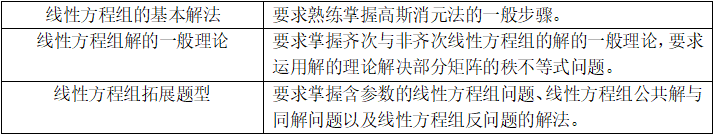
\includegraphics[scale=0.58]{8.png}
\end{figure}

\section{高斯消元法}
高斯消元法是考试中一定会考察的内容,无论是单独一个大题考察,还是嵌入在求解极大线性无关组等问题中。
注意单独考察解方程时,时间充足时建议将过程写完整,标明初等行变换的具体步骤,并且至少写出阶梯矩阵和行简化阶梯矩阵。
除此之外,需要保证计算中尽量减少错误,时间充足可以解完方程后将答案代入进行检查。

需要强调的是,不要认为本节内容很简单就放过了,实际上如果长期不计算高斯消元法很容易
造成眼高手低的窘境,因此希望各位同学熟悉高斯消元法的基本步骤并熟练应用。
\subsection{基本步骤}
一般的,对于一个由$m$个方程组成的$n$元(即变量数为$n$)线性方程组
$$\begin{cases}
	a_{11}x_1+a_{12}x_2+\cdots+a_{1n}x_n=b_1 \\
	a_{21}x_1+a_{22}x_2+\cdots+a_{2n}x_n=b_2 \\
	\cdots \\
	a_{m1}x_1+a_{m2}x_2+\cdots+a_{mn}x_n=b_m \\
\end{cases}$$
将其系数排列成矩阵
$$\begin{pmatrix}
	a_{11} & a_{12} & \cdots & a_{1n} \\
	a_{21} & a_{22} & \cdots & a_{2n} \\
	\cdots \\
	a_{m1} & a_{m2} & \cdots & a_{mn}
\end{pmatrix},$$
且记$\bm{b}=(b_1,b_2,\cdots,b_m)^\mathrm{T}$,若$\bm{b}=0$则称此方程为齐次线性方程组,否则为非齐次线性方程组。
再将$n$个未知量记为$n$元列向量$\bm{X}=(x_1,x_2,\cdots,x_n)^\mathrm{T}$,我们便可以把方程组简记为
$A\bm{X}=\bm{b}$.

令$\bm{\beta_i}=(a_{1i},a_{2i},\cdots,a_{mi})^\mathrm{T}$,即方程组系数矩阵的某一列,
则方程组还可以记为$x_1\bm{\beta_1}+x_2\bm{\beta_2}+\cdots+x_n\bm{\beta_n}=\bm{b}$,这一形式将在之后多次见到。

在以上的记号下,我们可以将解线性方程组的过程转化为矩阵的初等行变换。高斯消元法的一般步骤如下:

\centerline{线性方程组$\overset{1}{\longrightarrow}$增广矩阵$\overset{2}{\longrightarrow}$阶梯矩阵$\overset{3}{\longrightarrow}$(行)简化阶梯矩阵$\overset{4}{\longrightarrow}$解}

\begin{enumerate}
	\item 步骤1只需要将线性方程组转化为$(A, \bm{b})$的形式,得到左$n$列为系数矩阵,最后一列为列向量$\bm{b}$的$n+1$列的增广矩阵;
	\item 步骤2是通过初等行变换后,得到教材P34(1-13)的形式的矩阵——阶梯矩阵。阶梯矩阵系数全零行在最下方,并且非零行中,在下方的行的第一个非零元素一定在上方行的右侧(每行第一个非零元素称主元素);
	\item 步骤3将主元素化1后将主元素所在列的其他元素均通过初等行变换化为0即可;
	\item 步骤4中,我们分三种情况讨论:
	\begin{enumerate}
		\item 有唯一解:没有全零行,且行简化阶梯矩阵对角线上全为1,其余元素均为0,此时可以直接写出解;
		\item 无解:出现矛盾方程,即系数为0的行的行末元素不为0,此时直接写无解即可;
		\item 有无穷解:非上述情况。此时设出自由未知量将其令为$k_1,k_2,\cdots$然后代入增广矩阵对应的方程组即可。注意选取自由未知量时,选取没有主元素出现的列对应的未知量会与标准答案更贴近(如教材P33选取$x_2$、$x_5$),当然选择其他作为自由未知量也可以。
	\end{enumerate}
\end{enumerate}

\subsection{其他方法}
实际上我们还有其他方式解线性方程组,例如在系数矩阵可逆时直接求逆矩阵或者使用 Cramer 法则求解。
这些方法在之前相关章节已经讲述,此处不再展开。

\subsection{习题}
\centerline{\heiti A组}
\begin{enumerate}
	\item 求齐次线性方程组$\begin{cases}
		x_1+x_2+x_3+4x_4-3x_5=0 \\
		2x_1+x_2+3x_3+5x_4-5x_5=0 \\
		x_1-x_2+3x_3-2x_4-x_5=0 \\
		3x_1+x_2+5x_3+6x_4-7x_5=0
	\end{cases}$的通解.
	\item 求非齐次线性方程组$\begin{cases}
		x_1-x_2+2x_3-2x_4+3x_5=1 \\
		2x_1-x_2+5x_3-9x_4+8x_5=-1 \\
		3x_1-2x_2+7x_3-11x_4+11x_5=0 \\
		x_1-x_2+-x_3-x_4+3x_5=3
	\end{cases}$的通解.
	\item 求解线性方程组$\begin{cases}
		x_1+x_2+x_3=1 \\ x_1+2x_2-5x_3=2 \\ 2x_1+3x_2-4x_3=5
	\end{cases}$.
	\item 已知$V_1$是线性方程组$$\begin{cases}
		3x_1+4x_2-5x_3+7x_4=0 \\
		4x_1+11x_2-13x_3+16x_4=0
	\end{cases}$$
	的解空间,$V_2$是线性方程组$$\begin{cases}
		2x_1-3x_2+3x_3-2x_4=0 \\
		7x_1-2x_2+x_3+3x_4=0
	\end{cases}$$
	的解空间,分别求$V_1 \cap V_2$与$V_1+V_2$的基和维数.
	\item 设$A=\begin{pmatrix}
		1 & -1 & -1 \\ -1 & 1 & 1 \\ 0 & -4 & 2
	\end{pmatrix}$,$\xi_1=(-1,1,-2)^\mathrm{T}$.

	(1)求满足$A\xi_2=\xi_1$及$A^2\xi_3=\xi_1$的所有$\xi_2,\xi_3$;

	(2)证明:$\xi_1,\xi_2,\xi_3$线性无关.
\end{enumerate}

\section{线性方程组解的一般理论}
本节内容非常重要,一方面这是教材前六章的一大目标,即研究线性方程组不同解的情况
的来由;另一方面在于,这一节的内容在考试中经常出现,因此希望引起重视。

注意:本章在内容排布上与教材略有区别,但教材内容都会涉及。目的在于希望大家
不是死记硬背结论,而是能够遇到变式的定理都能理解并给出证明。如果希望先按照教材思路
回顾,实际上教材本章核心就在于定理6.1-6.3,应熟练掌握其证明并深刻理解其内涵。
\subsection{线性方程组解的一般理论}
\begin{theorem}
	(线性方程组有解的充要条件)线性方程组有解的充分必要条件是其系数矩阵与增广矩阵有相同的秩.
\end{theorem}
定理的证明非常简单,将方程组视为$x_1\bm{\beta_1}+x_2\bm{\beta_2}+\cdots+x_n\bm{\beta_n}=\bm{b}$,
则有解的条件为$\bm{b}$可以被$\bm{\beta_1},\cdots,\bm{\beta_n}$线性表示,这等价于
向量组$(\bm{\beta_1},\cdots,\bm{\beta_n})$与$(\bm{\beta_1},\cdots,\bm{\beta_n},\bm{b})$等价,故定理成立。

\begin{theorem}
	当方程组有解时(注意这个前提),以下定理成立:

	\textup{1} 如果它的系数矩阵$A$的秩等于未知量的数目$n$,则方程组有唯一解;
	
	\textup{2} 如果$A$的秩小于$n$,则方程组有无穷多个解.
\end{theorem}
这一定理有一个推论:齐次线性方程组有非零解的充要条件是:它的系数矩阵的秩小于未知量的数目(对于方阵即为行列式一章描述的,有非零解充分必要条件为其行列式为0)。
定理2对应齐次线性方程组即为教材定理6.1的推论,对于非齐次的情况,注意本定理前提是方程组有解。证明时将方程组化为简化阶梯矩阵即可。
\subsection{齐次线性方程组解的一般理论}
对于齐次线性方程组$AX=0$,我们有:
\begin{theorem}
	其解空间为$\mathbf{R}^n$的子空间。
\end{theorem}
请回顾证明子空间的一般方法。在确认其为线性空间后,我们来研究该线性空间的基本性质。首先是由此引出的关于基础解系的概念。
基础解系即为齐次线性方程组解空间的一组基,且这组基的每一个线性组合都是该方程组的解、
然后我们来研究这一空间的维数:
\begin{theorem}
	矩阵$A \in M_{m \times n}(\mathbf{F})$,若$r(A) = r$,则该齐次线性方程组解空间维数为$n - r$.
\end{theorem}
该定理即为教材定理6.1,证明使用维数公式(教材定理3.2)。本定理改写为类似于维数公式的形式即为$r(A) + \dim N(A) = n$。
其中$N(A)$表示$A\bm{X}=0$的解空间。
\begin{example}
	若$n$元齐次线性方程组$AX = 0$的解都是$BX = 0$的解,证明:$r(B) \le r(A)$.
\end{example}
\begin{theorem}
	$^*$齐次线性方程组解空间的正交补是由方程组行向量为基张成的线性空间.
\end{theorem}
该定理需要用到正交补的概念,没有学习的班级可以参考教材2.9节简单理解。实际上在矩阵的秩的讲义中已经提到了这一定理。
本定理中考虑了行向量张成的行空间,以往我们考虑列空间更多。

\subsection{非齐次线性方程组解的一般理论}
对于非齐次线性方程组
\begin{equation}
	x_1\bm{\beta_1}+x_2\bm{\beta_2}+\cdots+x_n\bm{\beta_n}=\bm{b}
\end{equation}
我们将n元齐次线性方程组
\begin{equation}
	x_1\bm{\beta_1}+x_2\bm{\beta_2}+\cdots+x_n\bm{\beta_n}=0
\end{equation}
称为其导出组,则我们有:
\begin{theorem}
	如果$n$元非齐次线性方程组有解,则它的解集$U=\{\gamma_0+\eta\ |\ \eta \in W\}$.
\end{theorem}
其中$\gamma_0$为(1)的一个解(称为特解),$W$为(2)的解空间((2)的解称为通解)。
对于通解+特解,我们可以想象一个3元非齐次线性方程$ax + by + cz = d$ 和齐次线性方程$ax + by + cz = 0$。
非齐次线性方程的解显然对应一个不过原点的平面,而齐次则过原点。
我们便可以认为是齐次线性方程解平面沿着特解对应的向量平移到非齐次线性方程的解平面,这便是这一结论的几何解释。同时我们可以得到下述结论:

1. $n$元非齐次线性方程组(1)的两个解的差是它的导出组(2)的一个解。

2. $n$元非齐次线性方程组(1)的一个解与它的导出组(2)的一个解之和仍是非齐次线性方程组(1)的一个解。

这两个性质证明比较简单,实际上根据上述几何描述形象理解也不困难。上述定理与性质对应教材定理6.3,可以参看。
\begin{example}
	设$n$阶矩阵$A$的行列式$|A|\neq 0$,记$A$的前$n-1$列形成的矩阵为$A_1$,$A$的第$n$列为$b$,
	问:线性方程组$A_1X=b$是否有解?
\end{example}

\subsection{习题}
\centerline{\heiti A组}
注意,A组习题中大部分题目都比较基础,或者直接就是教材或前面叙述的定理,所以如果有足够的自信可以只考虑思路,当然如果没有把握就请仔细写下证明。

证明以下关于线性方程组解的理论的基本定理:

第一组(齐次线性方程组解空间的一般理论)
\begin{enumerate}
	\item 设矩阵 $A \in M_{m\times n}(\mathbf{F})$,若 $r(A)=r$,则齐次线性方程组 $AX=0$ 的解空间 $N(A)$ 是 $\mathbf{F}^n$ 的一个 $n-r$ 维子空间.
	
	\item 设 $A$ 为 $m \times n$ 矩阵,则

		(1)齐次线性方程组 $AX=0$ 只有零解等价于 $r(A)=n$;
		
		(2)齐次线性方程组 $AX=0$ 有非零解(无穷解)等价于 $r(A)<n$.
	
	\item 设 $A$ 为 $n$ 阶矩阵,则

		(1)齐次线性方程组 $AX=0$ 只有零解等价于 $|A|\neq 0$;

		(2)齐次线性方程组 $AX=0$ 有非零解(无穷解)等价于 $|A|=0$.
	
	第二组(非齐次线性方程组解空间的一般理论)
	
	\item 对于非齐次线性方程组 $AX=b$,下列命题等价:
		
		(1)$AX=b$ 有解;
		
		(2)$b \in R(A)$,即 $b$ 可被 $A$ 的列向量组线性表示;
		
		(3)$r(A,b)=r(A)$,即增广矩阵的秩等于系数矩阵的秩.
	
	第三组(线性方程组解的结构的一般理论)
	
	\item 设 $X_1,\ X_2,\ \dots,\ X_s$ 为齐次线性方程组 $AX=0$ 的一组解,则 $k_1X_1+k_2X_2+\dots+k_sX_s$ 也为齐次线性方程组 $AX=0$ 的解,其中 $k_1,\ k_2,\ \dots,\ k_s$ 为任意常数.
	
	\item 设 $\eta_0$ 为非齐次线性方程组 $AX=b$ 的一个解,$X_1,\ X_2,\ \dots,\ X_s$ 为齐次线性方程组 $AX=0$ 的一组解,则 $k_1X_1+k_2X_2+\dots+k_sX_s+\eta_0$ 也为非齐次线性方程组 $AX=b$ 的解.
	
	\item 设 $\eta_1,\ \eta_2$ 为非齐次线性方程组 $AX=b$ 的两个解,则 $\eta_2-\eta_1$ 为齐次线性方程组 $AX=0$ 的解.
	
	\item 设 $X_1,\ X_2,\ \dots,\ X_s$ 为非齐次线性方程组 $AX=b$ 的一组解,则 $k_1X_1+k_2X_2+\dots+k_sX_s$ 也为非齐次线性方程组 $AX=b$ 的解的充分必要条件是 $k_1+k_2+\dots+k_s=1$.
	
	\item 设 $X_1,\ X_2,\ \dots,\ X_s$ 为非齐次线性方程组 $AX=b$ 的一组解,则 $k_1X_1+k_2X_2+\dots+k_sX_s$ 为齐次线性方程组 $AX=0$ 的解的充分必要条件是 $k_1+k_2+\dots+k_s=0$.
	
	判断以下关于线性方程组解的理论的说法是否正确并说明理由:
	
	第四组(一些经典的判断题)
	
	\item 方程组 $AX=b$ 有唯一解等价于方程组 $AX=0$ 只有零解.
	
	\item 设 $A$ 是 $m \times n$ 矩阵,$B$ 是 $n \times s$ 矩阵,若 $AB=O$,则 $B$ 的列向量为方程组 $AX=0$ 的解.
	
	\item 设 $A$ 是 $n$ 阶非零矩阵,则存在非零矩阵 $B$,使得 $AB=O$ 等价于 $r(A)<n$.
	
	\item 方程组 $AX=0$ 的解为 $BX=0$ 的解,则 $r(A)\ge r(B)$.
	
	\item 方程组 $AX=0$ 与 $BX=0$ 为同解方程组等价于 $r(A)=r(B)$.
	
	接下来为正常的练习题:

	\item 设$A$为四阶矩阵,$r(A)<4$,且$A_{21}\neq 0$,求方程组$AX=0$的通解.
	\item 设$A=(\alpha_1,\alpha_2,\alpha_3,\alpha_4)$为四阶矩阵,方程组$AX=0$的通解为$X=k(1,0,-4,0)^\mathrm{T}$,求
	$A^*X=0$的基础解系.
	\item 设$A$为$n$阶实矩阵,$W=\{\beta\in\mathbf{R}^n\ |\ \alpha^\mathrm{T}A\beta=0,\ \forall \alpha\in\mathbf{R}^n\}$,证明:
	
	(1)$\dim W+r(A)=n$;

	(2)$W$为$\mathbf{R}^n$的子空间.
	\item 已知4级方阵$A=(\alpha_1,\alpha_2,\alpha_3,\alpha_4)$的列向量$\alpha_1,\alpha_2,\alpha_4$线性无关,
	且$\alpha_1=2\alpha_2-\alpha_3$,若$\beta=\alpha_1-\alpha_2+3\alpha_4$,求方程组$AX=\beta$的通解.
	\item 设四元非齐次线性方程组的系数矩阵的秩为3,已知$\eta_1,\eta_2,\eta_3$是它的三个
	解向量,且$\eta_1=(2,3,4,5)^\mathrm{T},\eta_2+\eta_3=(1,2,3,4)^\mathrm{T}$,求该方程组的通解.
	\item 设$\beta_1,\beta_2,\beta_3$是$n$元非齐次线性方程组$AX=b$的三个线性无关的解,
	且$r(A)=n-2$,求:

	(1)导出组$AX=0$的一个基础解系;

	(2)$AX=2b$的一般解.
	\item 已知$A$是一个$s\times n$矩阵,证明:线性方程组$AX=b$对任意列向量$b_{s\times 1}$都有解的充要条件是$A$行满秩.
\end{enumerate}

\centerline{\heiti B组}
\begin{enumerate}
	\item 证明:若$X_0$是$AX=b$的一个特解,$X_1,\cdots,X_p$是$AX=0$的基础解系,
	证明:
	
	(1)$X_0,X_1,X_2,\cdots,X_p$线性无关;
	
	(2)$X_0,X_0+X_1,X_0+X_2,\cdots,X_0+X_p$线性无关;
	
	(3)$AX=b$的任一个解$X$可表示为
	$$X=k_0X_0+k_1(X_0+X_1)+k_2(X_0+X_2)\cdots+k_p(X_0+X_p),$$
	其中$k_0+k_1+k_2+\cdots+k_p=1$.
	\item 设$A$为$s \times n$矩阵,且$r(A)=r$,证明:非齐次线性方程组$AX=b$至多存在$n-r+1$个线性无关的解向量.
	\item 设$A$为$m \times n$矩阵,$r(A)=m$,$B$是$m$阶可逆矩阵,已知$A$的行空间$R(A^\mathrm{T})$是方程组$CX=0$的解空间,证明:
	$BA$的行向量也是$CX=0$的一个基础解系.
	\item 设$A$是$n$阶矩阵,且$A_{11}\neq 0$,证明:方程组$AX=b$($b$为非零向量)有无穷多解的充要条件为$A^*b=0$.
	\item 若$n$阶矩阵$A$的各行、各列元素之和都为0,证明:$A$的所有元素的代数余子式都相等.
	\item 已知 $\alpha_1,\ \alpha_2,\ \dots,\ \alpha_s$ 是齐次线性方程组 $AX=0$ 的一组基础解系,向量组

	$$
	\beta_1=t_1\alpha_1+t_2\alpha_2,\ \beta_2=t_1\alpha_2+t_2\alpha_3,\ \dots,\ \beta_{s-1}=t_1\alpha_{s-1}+t_2\alpha_s
	$$
	
	试问当实数 $t_1,\ t_2$ 满足何条件时,$AX=0$ 有基础解系包含向量 $\beta_1,\ \beta_2,\ \dots,\ \beta_{s-1}$,并写出该基础解系中的其余向量.
	\item (注:本题一般形式在教材第六章补充题1)已知线性方程组$$\begin{cases}
		a_{11}x_1+a_{12}x_2+\cdots+a_{1,2n}x_{2n}=0 \\
		a_{21}x_1+a_{22}x_2+\cdots+a_{2,2n}x_{2n}=0 \\
		\cdots \\
		a_{n1}x_1+a_{n2}x_2+\cdots+a_{n,2n}x_{2n}=0 \\
	\end{cases}$$
	的一个基础解系为$(b_{11},b_{12},\cdots,b_{1,2n})^\mathrm{T},\ (b_{21},b_{22},\cdots,b_{2,2n})^\mathrm{T},\ (b_{n1},b_{n2},\cdots,b_{n,2n})^\mathrm{T}$,
	求解线性方程组$$\begin{cases}
		b_{11}x_1+b_{12}x_2+\cdots+b_{1,2n}x_{2n}=0 \\
		b_{21}x_1+b_{22}x_2+\cdots+b_{2,2n}x_{2n}=0 \\
		\cdots \\
		b_{n1}x_1+b_{n2}x_2+\cdots+b_{n,2n}x_{2n}=0 \\
	\end{cases}.$$
	\item 设$A,B\in \mathbf{F}^{n\times n}$,且$r(A)=r$,$r(B)=s$,$r\begin{pmatrix}
		A \\ B
	\end{pmatrix}=k$.

	(1)证明:满足$AX=O$的$n$阶方阵$X$全体构成$\mathbf{F}^{n\times n}$的子空间,并求其维数;

	(2)令满足$AX=O$的$n$阶方阵$X$全体构成的子空间为$V_1$,满足$BX=O$的$n$阶方阵$X$全体构成的子空间为$V_2$,
	求$V_1+V_2$的维数.

	\item 设$A$是元素全为1的$n$阶方阵.
	
	(1)求行列式$|aE+bA|$,其中$a,b$为实常数;

	(2)已知$1<r(aE+bA)<n$,试确定$a,b$满足的条件,并求下列线性子空间的维数:
	$$W=\{x\ |\ (aE+bA)x=0,\ x\in\mathbf(R)\}.$$
	\item 已知线性方程组$$\begin{cases}
		a_{11}x_1+a_{12}x_2+\cdots+a_{1n}x_n=b_1 \\
		a_{21}x_1+a_{22}x_2+\cdots+a_{2n}x_n=b_2 \\
		\cdots \\
		a_{n1}x_1+a_{n2}x_2+\cdots+a_{nn}x_n=b_n \\
	\end{cases}$$
	的系数矩阵与
	$$\begin{pmatrix}
		a_{11} & a_{12} & \cdots & a_{1n} & b_1 \\
		a_{21} & a_{22} & \cdots & a_{2n} & b_2 \\
		\cdots \\
		a_{n1} & a_{n2} & \cdots & a_{nn} & b_n \\
		b_1 & b_2 & \cdots & b_n & 0
	\end{pmatrix},$$
	秩相等,求证:上述线性方程组有解.
	\item 设$A=(a_{ij})_{m\times n}$,$b$和$X$为$m$元列向量,$Y$为$n$元列向量,证明:
	
	(1)若$AY=b$有解,则$A^\mathrm{T}X=0$的任一组解都满足$b^\mathrm{T}X=0$;

	(2)方程组$AY=b$有解的充要条件是方程组$\begin{pmatrix}
		A^\mathrm{T} \\ b^\mathrm{T}
	\end{pmatrix}X=\begin{pmatrix}
		0 \\ 1
	\end{pmatrix}$无解(其中0是$n$元零向量).
\end{enumerate}

\centerline{\heiti C组}
\begin{enumerate}
	\item 用方程组的理论证明:一个$n$次多项式不可能有多于$n$个不同的根.
	\item 相容(即有解)的线性方程组$AX=b$在怎样的条件下,其解中第$k$个未知量$x_k$都是同一个值?
	你给的条件是否是充分必要的?
\end{enumerate}

\section{利用线性方程组解的一般理论解决矩阵秩的问题}
\subsection{概述}
我们首先来看四个最为经典的问题:
\begin{example}
	利用线性方程组解的一般理论,证明以下命题:
	
	\textup{(1)}设$A,B$分别是$m \times n$和$n \times s$矩阵,且$AB=O$,证明:$r(A)+r(B)\le n$\textup{;}

	\textup{(2)}设$A$是$m \times n$实矩阵,证明:$r(A^\mathrm{T}A)=r(A)$\textup{;}

	\textup{(3)}设$A,B$分别是$m \times n$和$n \times s$矩阵,则$r(AB)\le\min\{r(A),r(B)\}$\textup{;}

	\textup{(4)}$A^2=A \iff r(A)+r(E-A)=n$,$A^2=E \iff r(A+E)+r(A-E)=n$.
\end{example}
实际上,我们解决此类问题,很多时候等式都需要拆为小于等于和大于等于同时成立进行证明,经常利用
维数公式变形的齐次线性方程组解的一般理论,将问题转化为对像与核空间的研究,然后利用包含关系
(复杂的题目可能涉及子空间交与和的维数公式)以及已知的简单秩不等式进行证明。
可能部分题目较为困难,但至少请掌握上面例题中的情况。
\subsection{习题}
\centerline{\heiti A组}
\begin{enumerate}
	\item 设$A,B$分别是$m \times n$和$n \times s$矩阵,且$r(B)=n$,证明:若$AB=O$,则$A=O$.
\end{enumerate}
\centerline{\heiti B组}
\begin{enumerate}
	\item 判断:设 $A$ 是复数域上 $m \times n$ 阶矩阵,则矩阵秩 $r\left(A^T A\right)=r(A)$.
	\item 证明:对于$m \times n$实矩阵$A$,方程$A^\mathrm{T}AX = A^\mathrm{T}b$总是有解,且$A$为方阵时,$A^\mathrm{T}AX = 0$和$AX=0$同解.
	当$r(A)=n$时求其解,并证明$A(A^\mathrm{T}A)^{-1}A^\mathrm{T}$是幂等的对称矩阵.
	\item 设$A,B,C$为$n$阶实方阵,且$BAA^\mathrm{T}=CAA^\mathrm{T}$,证明:$BA=CA$.
	\item 设$A$为数域$\mathbf{F}$上的$n$阶方阵,又设线性空间$\mathbf{F^n}$的两个
	子空间为$W_1=\{X\in\mathbf{F}^n\ |\ AX=0\}$,$W_2=\{X\in\mathbf{F}^n\ |\ (A-E)X=0\}$.
	证明:$A^2=A \iff \mathbf{F}^n=W_1\oplus W_2$.
	\item $n$阶方阵$A$,$B$满足$AB=BA$,证明:$r(AB)+r(A+B)\le r(A)+r(B)$.
	\item 请按序证明以下结论:
	
	(1)$A,B$分别是$s \times m,m \times n$矩阵,则$ABX=0$与$BX=0$同解的充要条件是$r(AB)=r(B)$;

	(2)$A,B$分别是$s \times m,m \times n$矩阵,且$r(AB)=r(B)$,则对任意的$n \times t$矩阵都有$r(ABC)=r(BC)$;

	(3)设$A$是$n$阶方阵,则存在正整数$k$使得$r(A^k)=r(A^{k+1})=r(A^{k+2})=\cdots$,且对任意正整数$m$,有$r(A^n)=r(A^{n+m})$.
\end{enumerate}
\centerline{\heiti C组}
\begin{enumerate}
	\item 已知$A$是$n$阶对称矩阵,$\beta$为$n$元非零列向量,$B=\begin{pmatrix}
		A & \beta \\ \beta^\mathrm{T} & 0
	\end{pmatrix}$,证明:

	(1)若$r(A)=n$,则$B$可逆的充要条件是$\beta^\mathrm{T}A^{-1}\beta \neq 0$;

	(2)若$r(A)=r$,则$r(B)=r$的充要条件是方程组$\begin{cases}
		AX=\beta \\ \beta^\mathrm{T}X=0
	\end{cases}$有解;

	(3)若$r(A)=n-1$,则$B$可逆的充要条件是$AX=\beta$无解.
\end{enumerate}

\section{线性方程组拓展题型}
\subsection{含参数的线性方程组问题}
此类问题一般考察对于含参数的线性方程组,参数取值如何时有解/无解/有唯一解等。
此类问题一般有两种解法,一种是直接对系数矩阵做高斯消元法,另一种是考察系数矩阵行列式
是否为0(特别是系数矩阵行列式为n阶特殊行列式时)。当然考察系数矩阵行列式的方法不是
通用的,因为有时候参数不在系数矩阵,或者区分非齐次线性方程组无解/有无穷解的情况。
我们来看一个简单的例子:
\begin{example}
	讨论下面方程组的解的情况,并在有解的情况下求解:$$\begin{cases}
		x_1+x_2-x_3=1 \\ 2x_1+3x_2+kx_3=3 \\ x_1+kx_2+3x_3=2
	\end{cases}.$$
\end{example}
\subsection{线性方程组同解问题}
两个线性方程组同解实际上有两种情况:

1. 两线性方程组都无解;

2. 两线性方程组都有解且有相同的解集。

我们来看两线性方程组同解的充要条件:
\begin{theorem}
	$n$元齐次线性方程组($1$)$A_{m_1 \times n}X=0$与($2$)$B_{m_2 \times n}X=0$同解的
	充要条件是$r\begin{pmatrix}
		A \\ B
	\end{pmatrix}=r(A)=r(B)$.
\end{theorem}
\begin{theorem}
	$n$元非齐次线性方程组($1$)$A_{m_1 \times n}X=b$与($2$)$B_{m_2 \times n}X=d$同解的
	充要条件是
	
	\textup{1. }$r(A)\neq r(A,b)$且$r(B)\neq r(B,d)$
	
	或
	
	\textup{2. }r$\begin{pmatrix}
		A & b \\ B & d
	\end{pmatrix}=r\begin{pmatrix}
		A \\ B
	\end{pmatrix}=r(A)=r(A,b)=r(B)=r(B,d)$.
\end{theorem}
这两个定理的证明比较简单,作为练习。这两个定理可以用于两含参方程组同解问题的解决方法,当然应用前需要简要说明
以下这个定理。
\begin{example}
	已知方程组$$\begin{cases}
		x_1+2x_2+3x_3=0 \\ 2x_1+3x_2+5x_3=0 \\ x_1+x_2+ax_3=0
	\end{cases}$$
	与$$\begin{cases}
		x_1+bx_2+cx_3=0 \\ 2x_1+b^2x_2+(c+1)x_3=0
	\end{cases}$$
	同解,求$a,b,c$的值.
\end{example}
\subsection{线性方程组公共解问题}
公共解即为两线性方程组解集的交集,我们从齐次和非齐次讨论有公共解的条件:
\begin{theorem}
	对于$n$元齐次线性方程组\textup{(1)}$A_{m_1 \times n}X=0$与\textup{(2)}$B_{m_2 \times n}X=0$有

	\textup{(1)}\textup{(1)}与\textup{(2)}有非零公共解的充要条件是$r\begin{pmatrix}
			A \\ B
		\end{pmatrix}<n$\textup{;}

	\textup{(2)}设$\eta_1,\eta_2,\cdots,\eta_s(s=n-r(B))$是\textup{(2)}的基础解系,则
	\textup{(1)}与\textup{(2)}有非零公共解的充要条件是$A\eta_1,A\eta_2,\cdots,A\eta_s$线性相关\textup{;}

	\textup{(3)}设$\gamma_1,\gamma_2,\cdots,\gamma_t(t=n-r(A))$是\textup{(1)}的基础解系,
	$\eta_1,\eta_2,\cdots,\eta_s(s=n-r(B))$是\textup{(2)}的基础解系,则\textup{(1)}与\textup{(2)}有非零公共解的充要条件是
	$\gamma_1,\gamma_2,\cdots,\gamma_t,\eta_1,\eta_2,\cdots,\eta_s$线性相关.
\end{theorem}
\begin{theorem}
	对于$n$元非齐次线性方程组\textup{(1)}$A_{m_1 \times n}X=b$与\textup{(2)}$B_{m_2 \times n}X=d$,若\textup{(1)}与\textup{(2)}都有解,则

	\textup{(1)}\textup{(1)}与\textup{(2)}有公共解的充要条件是$r\begin{pmatrix}
			A \\ B
		\end{pmatrix}=r\begin{pmatrix}
			A & b \\ B & d
		\end{pmatrix}$\textup{;}

	\textup{(2)}若$r(B)=s$,且$\eta_1,\eta_2,\cdots,\eta_{n-s+1}$是\textup{(2)}的$n-s+1$个线性无关的解,则
	\textup{(1)}与\textup{(2)}有公共解的充要条件是$b$是$A\eta_1,A\eta_2,\cdots,A\eta_{n-s+1}$的凸组合,即
	存在数$k_1,k_2,\cdots,k_{n-s+1}$使得
	$$b=k_1A\eta_1+k_2A\eta_2+\cdots+k_{n-s+1}A\eta_{n-s+1},$$
	其中$k_1+k_2+\cdots+k_{n-s+1}=1$\textup{;}
	
	\textup{(3)}若$r(A)=t$,$r(B)=s$,$\gamma_1,\gamma_2,\cdots,\gamma_{n-t+1}$是\textup{(1)}的$n-t+1$个线性无关的解,
	$\eta_1,\eta_2,\cdots,\eta_{n-s+1}$是\textup{(2)}的$n-s+1$个线性无关的解,则\textup{(1)}与\textup{(2)}有公共解的充要条件是
	存在数$k_1,k_2,\cdots,k_{n-t+1}$和$l_1,l_2,\cdots,l_{n-s+1}$使得
	$$k_1\gamma_1+k_2\gamma_2+\cdots+k_{n-t+1}\gamma_{n-t+1}-l_1\eta_1-l_2\eta_2-\cdots-l_{n-s+1}\eta_{n-s+1}=0,$$
	其中$k_1+k_2+\cdots+k_{n-t+1}=1$,$l_1+l_2+\cdots+l_{n-s+1}=1$.
\end{theorem}
以上两个定理的证明作为练习。当然这两个定理无需记忆,只需要通过证明理解其含义即可。下面我们看一个简单的例子:
\begin{example}
	设四元齐次线性方程组\textup{(1)}为$$\begin{cases}
		2x_1+3x_2-x_3=0 \\ x_1+2x_2+x_3-x_4=0
	\end{cases}.$$已知另一个四元齐次线性方程组\textup{(2)}的基础解系为
	$$\alpha_1=(2,-1,a+2,1)^\mathrm{T},\alpha_2=(-1,2,4,a+8)^\mathrm{T}.$$

	\textup{(1)}求方程组\textup{(1)}的一个基础解系;

	\textup{(2)}当$a$为何值时,方程组\textup{(1)}和\textup{(2)}有非零公共解,并求出非零公共解.
\end{example}
\subsection{线性方程组反问题}
此类问题即已知方程组的解,要给出原方程组。对于齐次的情形,如果大家还记得系数矩阵行向量空间与解空间的
正交补关系,此类题目是容易解决的。对于非齐次线性方程组,则先利用通解得到其导出齐次线性方程组,然后将
特解代入得到需要求的非齐次线性方程组。
\begin{example}
	已知$\alpha_1=(1,2,-1,0,4)^\mathrm{T},\alpha_2=(-1,3,2,4,1)^\mathrm{T},\alpha_3=(2,9,-1,4,13)^\mathrm{T}$,
	且有$W=L(\alpha_1,\alpha_2,\alpha_3)$.

	\textup{(1)}求以$W$为解空间的一个齐次线性方程组;

	\textup{(2)}求以$W'=\{\eta+\alpha\ |\ \alpha\in W\}$为解集的一个非齐次线性方程组,其中$\eta=(1,2,1,2,1)^\mathrm{T}$.
\end{example}
\subsection{习题}
\centerline{\heiti A组}
\begin{enumerate}
	\item 设$A \in \mathbf{F}^{m \times n},B \in \mathbf{F}^{(n-m) \times n}(m<n)$,
	$V_1,V_2$分别为齐次线性方程组$AX=0$和$BX=0$的解空间,证明:$\mathbf{F}^n=V_1\oplus V_2$的解的
	充要条件是$\begin{pmatrix}
		A \\ B
	\end{pmatrix}X$=0只有零解.

	注:本题是吴志祥老师2020-2021期中考试第一题的解题原理,但那题数据凑得不好因此是个错题,
	所以我们没有给具体的例子,而是给出原理要求证明,希望同学们碰到两方程组解空间互为补空间
	的题目会用这种方式解决.
	\item 齐次线性方程组$$\begin{cases}
		x_2+ax_3+bx_4=0 \\ -x_1+cx_3+dx_4=0 \\ ax_1+cx_2-ex_4=0 \\ bx_1+dx_2+ex_3=0
	\end{cases}$$
	的一般解以$x_3,x_4$作为自由未知量.

	(1)求$a,b,c,d,e$满足的的条件;

	(2)求齐次线性方程组的基础解系.
\end{enumerate}

\centerline{\heiti B组}
\begin{enumerate}
	\item 如果齐次线性方程组$$\begin{cases}
		x_1+x_2+bx_3-x_4+x_5=0 \\
		2x_1+3x_2+x_3+x_4-2x_5=0 \\
		x_2+ax_3+3x_4-4x_5=0 \\
		-3x_1-3x_2-3bx_3+bx_4+(a+2)x_5=0
	\end{cases}$$
	的解空间是3维的,试求$a,b$的值与解空间的基,解空间可能为2维吗?
	\item 设$W_1,W_2$分别为$n$元齐次线性方程组$AX=0$和$BX=0$的解空间,试构造两个$n$元
	齐次线性方程组,使它们的解空间分别为$W_1 \cap W_2$和$W_1+W_2$.
	\item 已知方程组$$\begin{cases}
		x_1+x_2+ax_3+x_4=1 \\ -x_1+x_2-x_3+bx_4=2 \\ 2x_1+x_2+x_3+x_4=c
	\end{cases}$$与$$\begin{cases}
		x_1+x_4=-1 \\ x_2-2x_4=d \\ x_3+x_4=e
	\end{cases}$$同解,求$a,b,c,d,e$.
	\item 设有两个非齐次线性方程组(1)和(2),它们的通解分别是$X=\gamma+t_1\eta_1+t_2\eta_2=\delta+k_1\xi_1+k_2\xi_2$.
	其中$\gamma=(5,-3,0,0)^\mathrm{T},\eta_1=(-6,5,1,0)^\mathrm{T},\eta_2=(-5,4,0,1)^\mathrm{T},
	\delta=(-11,3,0,0)^\mathrm{T},\xi_1=(8,-1,1,0)^\mathrm{T},\xi_2=(10,-2,0,1)^\mathrm{T}$,求这两个方程组的公共解.
	\item 若方程组$$\begin{cases}
		x_1+x_2+x_3=0 \\ x_1+2x_2+ax_3=0 \\ x_1+4x_2+a^2x_3=0
	\end{cases}$$与$$x_1+2x_2+x_3=a-1$$有公共解,求$a$的值及所有公共解.
\end{enumerate}

\centerline{\heiti C组}
\begin{enumerate}
	\item 讨论$b_1,b_2,\cdots,b_n(n\ge 2)$满足什么条件时,下列方程组$$\begin{cases}
		x_1+x_2=b_1 \\ x_2+x_3=b_2 \\ \cdots \\ x_{n-1}+x_n=b_{n-1} \\ x_n+x_1=b_n
	\end{cases}$$有解,并求解.
	\item 已知$A$是$s \times n$矩阵,$B$是$m \times n$矩阵,$X,a,b$分别是$n,s,m$元列向量,证明:
	
	(1)齐次线性方程组$AX=0$和$BX=0$同解的充要条件是$A$与$B$行向量等价(列向量不一定);

	(2)齐次线性方程组$AX=0$和$BX=0$解空间分别为$V_1,V_2$,证明:$V_1 \subseteq V_2$的充要条件是存在$m \times s$
	矩阵$C$使得$B=CA$;

	(3)线性方程组$AX=a$的解都是$BX=b$的解的充要条件是增广矩阵$(B,b)$的每个行向量都可以被$(A,a)$的行向量线性表示;

	(4)线性方程组$AX=a$与$BX=b$同解的充要条件是$(A,a)$与$(B,b)$行向量等价.
\end{enumerate}

\chapter{特征值与特征向量\ 矩阵标准形}

\section{Overview}
\begin{figure}[h]
	\centering
	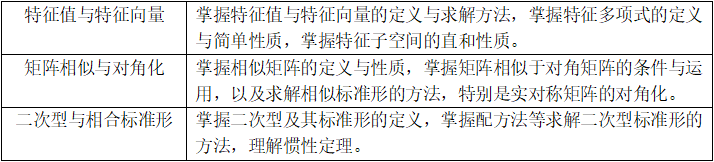
\includegraphics[scale=0.58]{9.png}
\end{figure}
注:由于本学期正交以及正定内容部分班级未讲授,因此也没有包含在本讲义中.讲义中可能有少量(2-3题)涉及
二次型正交标准化方法,可以简要了解或略过.
\section{特征值与特征向量}
从本章起,我们主要研究线性变换(而非一般线性映射)和方阵的性质.
\subsection{特征值与特征向量的定义与求解}
首先介绍线性变换和矩阵的特征值与特征向量的概念:
\begin{definition}
	设$\sigma$是线性空间$V(\mathbf{F})$上的一个线性变换,如果存在数$\lambda\in\mathbf{F}$
	和非零向量$\xi\in V$使得$\sigma(\xi)=\lambda\xi$,则称数$\lambda$为$\sigma$的一个特征值,
	并称非零向量$\xi$为$\sigma$属于其特征值$\lambda$的特征向量.
\end{definition}
必须注意特征向量为非零向量,否则零向量对任意$\lambda$都满足上面定义,从而失去“特征”的含义.
但是特征值可以为0,此时实际上就是线性变换的零空间.

特征值与特征向量的几何意义在于,某一线性变换的特征向量在经过变换后得到的向量与原先向量共线.

我们称关于同一个特征值$\lambda$的所有特征向量构成的集合记为$V_\lambda=\{\xi\ |\ \sigma(\xi)=\lambda\xi,\xi\in V\}$,
称为$\sigma$关于其特征值$\lambda$的特征子空间.
\begin{example}
	证明:$V_\lambda$是$V$的子空间.
\end{example}
实际上,$\sigma(\xi)=\lambda\xi$等价于$(\lambda I-\sigma)(\xi)=0$,故特征子空间就是线性变换
$\lambda I-\sigma$的核,核中必有非零向量(特征向量非零),故$\lambda I-\sigma$在$\lambda$为特征值时
必不满秩,故我们可以通过$|\lambda E-A|=0$求解特征值,其中$A$为$\sigma$在某组基下的矩阵.
对于特征向量的求解,求出$(\lambda E-A)X=0$的非零解就是特征向量在基下的坐标.

上面是线性变换的特征值与特征向量的定义,我们在考试中更一般地会遇到下述矩阵的特征值与特征向量的定义:
\begin{definition}
	设矩阵$A\in M_n(\mathbf{F})$,如果存在数$\lambda\in\mathbf{F}$和非零向量$X\in\mathbf{F}^n$使得
	$AX=\lambda X$,则称数$\lambda$为$A$的一个特征值,称非零向量$X$为$A$属于其特征值$\lambda$的特征向量.
\end{definition}
\begin{example}
	设$A=\begin{pmatrix}
		1 & -1 & 0 \\ 2 & 0 & 1 \\ 1 & a & 0
	\end{pmatrix}$,且存在非零向量$\alpha$使得$A\alpha=2\alpha$,求$\alpha$.
\end{example}
下面我们说明这两个定义的关系.实际上,假设$A$是$\sigma$在基$\alpha_1,\cdots,\alpha_n$下的表示矩阵,且
$\xi=(\alpha_1,\cdots,\alpha_n)X$,我们有
\begin{align*}
	\sigma(\xi)=\lambda\xi &\Leftrightarrow \sigma(\alpha_1,\cdots,\alpha_n)X=\lambda(\alpha_1,\cdots,\alpha_n)X \\
						   &\Leftrightarrow (\alpha_1,\cdots,\alpha_n)AX=(\alpha_1,\cdots,\alpha_n)(\lambda X) \\
						   &\Leftrightarrow AX=\lambda X
\end{align*}
因此$\lambda$同时是线性变换和矩阵的特征值,与基的选取无关,但$X$与基的选取有关.

我们在之前已经分析了求解特征值的方法,即求解$f(\lambda)=|\lambda E-A|$的根. 我们称其为矩阵$A$的特征多项式.
其$k$重根称为$k$重特征值(或称代数重数),对应的特征子空间维数称几何重数.

我们展开特征多项式得到以下定理:
\begin{theorem}
	对于$n$级矩阵$A=(a_{ij})$,记
	$$f(\lambda)=|\lambda E-A|=a_0\lambda^n+a_1\lambda^{n-1}+\cdots+a_{n-1}\lambda+a_n.$$
	则$a_0=1$,$a_n=(-1)^n|A|$,且$a_k$等于所有$k$级主子式之和乘以$(-1)^k$.
\end{theorem}
这一定理的证明无需掌握,并且关于特征多项式的进一步讨论也将在线性代数II中涉及.这里我们主要掌握两个特例,
即由韦达定理,我们有$\sum\limits_{i=1}^{n}\lambda_i=\sum\limits_{i=1}^{n}a_{ii}$,
$\prod\limits_{i=1}^{n}\lambda_i=|A|$,
即特征值按重数求和为矩阵的迹(即矩阵对角线元素之和),特征值按重数求积为矩阵行列式.
这一结论在解决某些问题时有一定作用.

\subsection{特征值的基本性质}
关于特征值,我们有如下基本性质,证明较为基本,可以自行完成:

设$\lambda$是线性空间$V(\mathbf{F})$上的线性变换$\sigma$的特征值,$\xi$是$\sigma$属于$\lambda$的特征向量,则

1. $k\lambda$是$k\sigma$的特征值,$\lambda^m$是$\sigma^m$的特征值,且$\xi$仍是相应特征向量.

2. 若$f(x)=a_nx^n+a_{n-1}x^{n-1}+\cdots+a_1x+a_0$是$\mathbf{F}$上的多项式,则$f(\sigma)(\xi)=f(\lambda)\xi$.

3. 设$\lambda$是$n$阶矩阵$A$的特征值,$A$可逆,则$\lambda^{-1}$是$A^{-1}$的特征值,$|A|\lambda^{-1}$是$A$的伴随矩阵
$A^*$的特征值,且特征向量不变.
\begin{example}
	回答以下问题:

	\textup{(1)}设$A$为三阶矩阵,$A^2-A-2E=O$,$|A|=2$,求$|A^*+3E|$\textup{;}
	
	\textup{(2)}设$A$为三阶矩阵,其特征值为$1$,$-2$,$-1$,求$|A|$,$A^*+3E$的特征值,$(A^{-1})^2+2E$的特征值
	以及$|A^2-A+E|$\textup{;}
	
	\textup{(3)}设$\alpha=(1,0,-1)^\mathrm{T}$,且$A=\alpha\alpha^\mathrm{T}$,求$|6E-A^n|$\textup{;}
	
	\textup{(4)}设$A$为三阶矩阵,其特征值为$-1$,$-1$,$5$,求$A_{11}+A_{22}+A_{33}$\textup{;}
	
	\textup{(5)}设$A$为三阶实对称矩阵,$A^2=A$且$r(A)=2$,求$|A+2E|$.
\end{example}

下面一个例子也是重要的结论,实际上在行列式专题已给出类似结论,但我们现在从特征值角度考虑这一结论:
\begin{example}
	回答以下两个问题:
	
	\textup{(1)}设$A,B$均为$n$阶矩阵,证明:$\lambda\neq 0$是$AB$的特征值,则$\lambda$也是$BA$的特征值\textup{;}
	
	\textup{(2)}设$A\in M_{m\times n}(\mathbf{C}),B\in M_{n\times m}(\mathbf{C})$,证明:
	$$\begin{pmatrix}
		AB & O \\ B & O
	\end{pmatrix}\sim\begin{pmatrix}
		O & O \\ B & BA
	\end{pmatrix},$$
	并由此推出$AB$和$BA$非零特征值相同,且$m=n$时有$|\lambda E-AB|=|\lambda E-BA|$.
\end{example}
不难发现(2)是(1)的推广.下面这一例子也是一些经典的结论,应当熟悉.
\begin{example}
	对下列矩阵$A$的特征值,能做出怎样的断言?
	
	\textup{(1)}$A$可逆/$A$不可逆/$E+A$可逆/$4E+A$不可逆\textup{;}
	
	\textup{(2)}$\det(E-A^2)=0$\textup{;}
	
	\textup{(3)}$AA^\mathrm{T}=A^\mathrm{T}A=E$(正交)/$A^2=E$(对合)/$A^2=A$(幂等)/$A^k=0$(幂零)\textup{;}
	
	\textup{(4)}$A=\lambda_0E+B$($\lambda_0$为常数,且已知$B$的$n$个特征值为$\lambda_1,\lambda_2,\cdots,\lambda_n$)\textup{;}
	
	\textup{(5)}$A$为对角块矩阵,即$A=\begin{pmatrix}
		A_1 &  &  &  \\  & A_2 &  &  \\  &  & \ddots &  \\  &  &  & A_m
	\end{pmatrix}$(与线代$\textup{II}$中不变子空间有关).
\end{example}
在上一小节我们讨论了特征值之和为迹的事实,实际上关于迹以及相关的幂零矩阵的讨论在专题三中已有涉及,
现在可以回过头去再看一些性质的证明.除此之外,我们还可以给幂零矩阵一个等价的定义:
\begin{theorem}
	一个方阵为幂零矩阵当且仅当其所有特征值均为$0$.
\end{theorem}
这一定理“仅当”部分证明比较基本,只需用到上述某一特征值性质即可,但“当”的部分无需掌握证明,需要用到线性代数II的
哈密顿-凯莱定理(事实上很多更进一步的讨论都要基于这一定理).
\subsection{特征向量的基本性质}
这一部分的定理与下一节中可对角化的等价条件直接相关,实际上有了本节的定理,可对角化条件是很显然的.
\begin{theorem}
	线性映射$\sigma$的不同特征值$\lambda_1,\cdots,\lambda_m$对应的特征向量$\xi_1,\cdots,\xi_m$线性无关.
\end{theorem}
\begin{theorem}
	线性映射$\sigma$的不同特征值$\lambda_1,\cdots,\lambda_m$对应的特征子空间$V_{\lambda_1},\cdots,V_{\lambda_m}$的和是直和,
	即$\dim(V_{\lambda_1}+V_{\lambda_2}+\cdots+V_{\lambda_m})=\sum_{j=1}^{m}\dim V_{\lambda_j}$.
\end{theorem}
以上两个定理的证明可以参考教材定理7.7及其推论,实际上二者等价,只需证出其中一个,另一个就是显然的.
两个定理有如下推论:

1. 若$\lambda_1,\cdots,\lambda_m$是线性映射$\sigma$互异的特征值,则$V_{\lambda_i}\cap\sum\limits_{j\neq i}V_{\lambda_j}=\{0\}
(i=1,\cdots,m)$,则一个特征向量不能属于多个特征值.这一推论来源于直和的一个等价条件,专题一的习题中有涉及.

2. $\sigma$的不同特征值$\lambda_1,\cdots,\lambda_m$对应的特征子空间$V_{\lambda_1},\cdots,V_{\lambda_m}$的基向量
合在一起构成的向量组线性无关,且是$V_{\lambda_1}+V_{\lambda_2}+\cdots+V_{\lambda_m}$的基.

接下来这个定理说明了代数重数和几何重数之间的关系:
\begin{theorem}
	$n$维线性空间$V(\mathbf{F})$的线性变换$\sigma$的每个特征值$\lambda_i$的重数(代数重数)大于等于其特征子空间$V_{\lambda_i}$的维数
	(几何重数).
\end{theorem}
这一定理的证明比较复杂,版本也很多,有兴趣的同学可以了解.
\subsection{习题}
\centerline{\heiti A组}
\begin{enumerate}
	\item 设$\sigma$是线性空间$\mathbf{R}[x]_3$上的线性变换,它在基$1,x,x^2$下的矩阵为
	$$A=\begin{pmatrix}
		1 & 2 & 2 \\ 2 & 1 & 2 \\ 2 & 2 & 1
	\end{pmatrix}.$$
	求$\sigma$的特征值与特征子空间.
	\item 设$A,P$都是3阶方阵,$P$可逆,已知$A$的特征值$\lambda_1=1,\lambda_2=-1,\lambda_3=2$,$B=A^3-5A^2$,
	求$|B|$,$|A+5E|$,$|5E+P^{-1}AP|$.
	\item 设$A=\begin{pmatrix}
		a & -1 & c \\ 5 & b & 3 \\ 1-c & 0 & -a
	\end{pmatrix}$,$|A|=-1$,$\alpha=(-1,-1,1)^\mathrm{T}$为$A^*$的特征向量,求$A^*$的特征值及$a,b,c$
	和$A$对应的特征值$\mu$.
	\item 设$A,B\in M_n(\mathbf{F})$,$AB=BA$,证明:若$X$是矩阵$A$属于特征值$\lambda_0$的特征向量,则
	$BX\in V_{\lambda_0}$(注:本题是解决很多$AB=BA$类问题的基础).
\end{enumerate}
\centerline{\heiti B组}
\begin{enumerate}
	\item 设$A,B$都是$n$阶矩阵,且$r(A)+r(B)<n$,证明:$A,B$有相同的特征值和特征向量.
	\item 设$V(\mathbf{F})$是$n$维线性空间,$\sigma\in L(V,V)$,证明:
	
	(1)若$\alpha,\beta$是$\sigma$的属于不同特征值的特征向量,则$c_1c_2\neq 0$时,$c_1\alpha+c_2\beta$
	不是$\sigma$的特征向量;

	(2)$V$中的每一非零向量都是$\sigma$的特征向量$\iff\sigma=c_0I_V$,其中$c_0\in\mathbf{F}$是一个常数,
	$I_V$是恒等变换.
	\item 设$A,B\in M_n(\mathbf{C})$,$B$的特征多项式$f(\lambda)=|\lambda E-B|$.证明:$f(A)$可逆的充要条件
	是$B$的任一特征值都不是$A$的特征值.
	\item 设$\lambda_1,\lambda_2,\cdots,\lambda_n$是矩阵$A=(a_{ij})_{n\times n}$的$n$个特征值,证明:
	$\lambda_1^2,\lambda_2^2,\cdots,\lambda_n^2$是$A^2$的$n$个特征值,且$\sum\limits_{i=1}^{n}\lambda_i^2=
	\sum\limits_{j=1}^{n}\sum\limits_{k=1}^{n}a_{jk}a_{kj}$.
	\item 设$A$为$n$阶矩阵,$X_1,X_2,X_3$为$n$元列向量,且$AX_1=kX_1(X_1\neq 0),AX_2=lX_1+kX_2,
	AX_3=lX_2+kX_3(l\neq 0)$,证明:$X_1,X_2,X_3$线性无关.
\end{enumerate}
\centerline{\heiti C组}
\begin{enumerate}
	\item 证明:若$AB=BA$,则$A$和$B$至少有一个共同的特征向量.
\end{enumerate}

\section{矩阵相似与对角化}
\subsection{矩阵相似的定义与性质}
我们早在线性映射矩阵表示专题中提到这一定理:
\begin{theorem}
	\textbf{基的选择对映射矩阵的影响}
	
	设线性变换$\sigma \in L(V,V)$,$B_1=\{\alpha_1,\dots,\alpha_n\}$和$B_2=\{\beta_1,\dots,\beta_n\}$
	是线性空间的$V(F)$的两组基,基$B_1$变为基$B_2$的变换矩阵为$C$,如果$\sigma$在基$B_1$下的矩阵为$A$,
	则$\sigma$关于基$B_2$所对应的矩阵为$C^{-1}AC$.
\end{theorem}
定理相关习题在相关章节有介绍,教材也有例题.这一定理研究同一个映射在不同基下表示矩阵之间的关系.
我们将具有如上性质的两个矩阵的关系称为相似的,规范定义如下:
\begin{definition}
	若对于$A,B\in M_n(\mathbf{F})$,存在可逆矩阵$C\in M_n(\mathbf{F})$, 使得
	$C^{-1}AC=B$,则称$A$相似于$B$,记作$A\sim B$.
\end{definition}
相似矩阵有以下基本性质,证明较为基本,请自行完成:

1. 相似是一种等价关系;两矩阵相似必相抵(秩相等);

2. $A\sim B$可以得到$A^\mathrm{T}\sim B^\mathrm{T}$,$A^m\sim B^m$,更一般地,对于任意多项式$f(x)$都有$f(A)\sim f(B)$,且
若$B=P^{-1}AP$,有$f(B)=P^{-1}f(A)P$.除此之外还有$A^*\sim B^*$,若$A,B$可逆,有$A^{-1}\sim B^{-1}$,$A^*\sim B^*$;

3. $A_1\sim B_1$,$A_2\sim B_2$不一定有$A_1+A_2\sim B_1+B_2$,只有当$P^{-1}A_1P=B_1,P^{-1}A_2P=B_2$时
(即相同的过渡矩阵$P$)才有$P^{-1}(A_1+A_2)P=B_1+B_2$;

4. 若$A_1\sim B_1$,$A_2\sim B_2$,则有
$$\begin{pmatrix}
	A_1 & O \\ O & A_2
\end{pmatrix}\sim\begin{pmatrix}
	B_1 & O \\ O & B_2
\end{pmatrix}\textup{;}$$

5. 相似矩阵有相同的特征多项式(逆命题不成立),即$A\sim B$有$|\lambda E-A|=|\lambda E-B|$,从而有相同的
迹,行列式,特征值,但特征向量不一定相同;

6. 与幂等矩阵相似的仍幂等,与对合矩阵相似的仍对合,与幂零矩阵相似的仍幂零
(但与正交矩阵相似的不一定正交,但与正交矩阵正交相似的是正交矩阵).
\begin{example}
	证明:两个可对角化的同阶矩阵特征值相同(包括重数)等价于它们相似.对于不可对角化的矩阵来说,这一结论还成立吗?
\end{example}
\begin{example}
	(教材定理$4.10$推广)设$P^{-1}AP=B$,证明:$A,B$分别属于同一特征值$\lambda$的特征向量$X$和$Y$满足$Y=P^{-1}X$.
\end{example}
一些题目可能需要判断矩阵是否相似,实际上我们有如下基本方法:
\begin{enumerate}
	\item 定义法:找到$P$使得$P^{-1}AP=B$即可,这一般是$A,B$没给出具体矩阵的做法,例如上面的性质证明;
	\item 我们也可以先计算两者特征多项式是否相等(即特征值是否一致),若不一致则一定不相似,得到结论,若一致且均为实对称矩阵则相似,
	否则不一定相似.于是对于这种特征值一致的情况,我们进行对角化,情况如下:
	\begin{enumerate}
		\item 若两矩阵均可对角化,则两矩阵相似(上述例题结论);
		\item 若一个矩阵可对角化,另一个矩阵不可对角化,则一定不相似;
		\item 若两个矩阵都不可对角化,不一定相似.需要两矩阵各个特征值的几何重数(即各个特征子空间维数)都一致才相似,否则不相似
		(了解结论即可,具体原因线性代数II会涉及).
	\end{enumerate}
\end{enumerate}
\begin{example}
	设$A,B\in M_n(\mathbf{F})$,证明:若$A$可逆,则$AB\sim BA$.
\end{example}
\begin{example}
	设$A=\begin{pmatrix}
		0 & 0 & 1 \\ 0 & 1 & 0 \\ 1 & 0 & 0
	\end{pmatrix},B=\begin{pmatrix}
		-1 & 0 & 0 \\ 0 & 0 & 1 \\ 0 & -1 & 2
	\end{pmatrix}$,判断$A$与$B$是否相似.
\end{example}
最后我们谈一个拓展内容,我们考虑矩阵方程$AX-XB=O$,若$A,B$都是$n$阶方阵且$X$可逆,则$A$与$B$相似,所以
这一矩阵方程的解空间的维数实际上刻画了$A$与$B$的相似程度.我们有如下结论,不要求掌握,也不要求证明,了解即可:
\begin{theorem}
	设$A,B$分别为数域$P$上$n$阶、$m$阶方阵,则$A,B$有$r$个两两不等的公共特征值,则矩阵方程$AX-XB=O$有秩为
	$r$的矩阵解.反之,若数域为复数域,矩阵方程$AX-XB=O$有秩为$r$的矩阵解,则$A,B$至少有$r$个公共的特征值
	(计重数).
\end{theorem}
由此,复数域上$n$阶、$m$阶方阵$A,B$的矩阵方程$AX=XB$只有零解的充要条件是$A,B$没有公共特征值.
\subsection{可对角化的条件}
我们知道,矩阵可对角化意味着矩阵相似于一个对角矩阵,即存在可逆矩阵$P$使得$P^{-1}AP=\Lambda$,其中
$\Lambda=\textup{diag}(\lambda_1,\lambda_2,\cdots,\lambda_n)$为对角矩阵.

将$P^{-1}AP=\Lambda$变形为$AP=P\Lambda$,并将矩阵$P$按列分块为$P=(X_1,X_2,\cdots,X_n)$,则有
$A(X_1,X_2,\cdots,X_n)=(X_1,X_2,\cdots,X_n)\textup{diag}(\lambda_1,\lambda_2,\cdots,\lambda_n)$,
利用分块矩阵乘法我们有$AX_j=\lambda_jX_j(X_j\neq 0,j=1,2,\cdots,n)$.

通过上述过程我们容易证明$n$维空间上线性映射可对角化当且仅当有$n$个线性无关的特征向量.并且这一过程也是我们
求解对角化问题的基本方法.综合上述推导以及上一节中2.3小节的定理,我们有如下结论:
\begin{theorem}
	设$V$是数域$\mathbf{F}$上的$n$维线性空间,$\sigma$是$V$上的线性变换,$\lambda_1,\lambda_2,\cdots,\lambda_s\in\mathbf{F}$
	是$\sigma$的所有互异特征值,则以下条件等价:
	
	\textup{(1)}$\sigma$可对角化\textup{;}
	
	\textup{(2)}$\sigma$有$n$个线性无关的特征向量,它们构成$V$的一组基\textup{;}
	
	\textup{(3)}$V=V_{\lambda_1}\oplus V_{\lambda_2}\oplus\cdots\oplus V_{\lambda_s}$\textup{;}
	
	\textup{(4)}$n=\dim V_{\lambda_1}+\dim V_{\lambda_2}+\cdots+\dim V_{\lambda_s}$\textup{;}
	
	\textup{(5)}$\sigma$每个特征值的代数重数等于几何重数\textup{.}
\end{theorem}
实际上对于矩阵我们有对应的定理,此处不再赘述.我们有一个推论,若有$n$个互不相同的特征值则一定能对角化,
这是(2)的直接推论,但反之不成立,有多重特征值的矩阵也可能可以对角化,只要满足上述条件.

实际上由特征值的性质,我们容易知道数域$\mathbf{F}$上矩阵$A$可对角化,则$A^*$可对角化,对于数域$\mathbf{F}$上
任意多项式$f(x)$,$f(A)$也可对角化,且$A$可逆时,$A^{-1}$也可对角化.
\begin{example}
	证明$r$阶上三角矩阵$(r>1)$
	$$J_0=\begin{pmatrix}
		\lambda_0 & 1 &  &  \\ 
		  & \lambda_0 & \ddots &  \\
		  &  & \ddots &  1 \\
		  &  &  &  \lambda_0
	\end{pmatrix}$$
	不与对角阵相似.
\end{example}
\begin{example}
	设$A=(a_{ij})_{n\times n}$是上三角矩阵.
	
	\textup{(1)}求$A$的全部特征值\textup{;}

	\textup{(2)}若$A$主对角元互不相等,证明:$A$与对角阵相似\textup{;}

	\textup{(3)}若$n$个主对角元相等且$A$不为对角矩阵,证明:$A$不与对角阵相似.
\end{example}
\begin{example}
	设$\alpha$和$\beta$是$\mathbf{R}^n(n>1)$中两个列向量,$A=\alpha\beta^\mathrm{T}\neq O$.
	
	\textup{(1)}求$A$的特征值\textup{;}
	
	\textup{(2)}证明:$\alpha^\mathrm{T}\beta=0\iff A$不可对角化.
\end{example}
最后需要说明一点,如果一个矩阵可对角化,那么我们可以将其表示为$A=P\Lambda P^{-1}$,其中
$P$可逆(即所谓特征值分解).实际上相抵、相合都有类似的表示思想,在解决一些题目时是重要的.
\begin{example}
	设$n$阶实对称矩阵$A$的特征值$\lambda_i\ge 0(i=1,\cdots,n)$.证明:存在特征值都是非负数的实对称矩阵
	$B$使得$A=B^2$(本题可推广为多次幂).
\end{example}
\begin{example}
	设三阶矩阵$A$的特征值为$\lambda_1=-2,\lambda_2=1,\lambda_3=2$,对应的特征向量分别为
	$\alpha_1=(1,1,0)^\mathrm{T},\alpha_2=(1,0,1)^\mathrm{T},\alpha_3=(1,1,1)^\mathrm{T}$,求矩阵$A$.
\end{example}
\subsection{对角化问题的一般解法}
下面我们总结一下求解对角化问题的基本方法:对于一个$n$阶可对角化矩阵$A$,求变换矩阵$P$使得$P^{-1}AP=\Lambda$,步骤如下:

1. 求出$A$的所有不同特征值;

2. 求出$A$在不同特征值下的特征子空间的基;

3. 将这组基按列排列成矩阵$P$.

这一过程的合理性在本小节开头就有叙述.下面我们来看一个基本的例子:
\begin{example}
	设$A=\begin{pmatrix}
		2 & 2 & 0 \\ 8 & 2 & a \\ 0 & 0 & 6
	\end{pmatrix}$相似于对角矩阵,求常数$a$,并求可逆矩阵$P$使得$P^{-1}AP$为对角矩阵.
\end{example}
除此之外,我们还可以利用对角化求解矩阵的幂的问题,在专题三中已经介绍,此处不再赘述.

\subsection{实对称矩阵对角化}
这一部分内容因为涉及正交的概念所以有班级未提及,因此我们只能回顾不涉及正交的部分.
教材定义7.7给出了共轭矩阵的概念,下方给出了大量的性质,此处不再赘述.我们的重点在于以下两个定理:
\begin{theorem}
	实对称矩阵的特征值都是实数.
\end{theorem}
这一定理的证明应当掌握,特别是如何证明实数的方法(即共轭等于自身).
\begin{theorem}
	实对称矩阵一定可以相似对角化.
\end{theorem}
这一定理证明只需要讲教材定理7.13除去正交即可.以上两个定理十分重要,是我们接下来讨论以及解决一些问题的基础.
\begin{example}
	已知$A$是实反对称矩阵,证明:

	\textup{(1)}$A$的特征值必为$0$或纯虚数\textup{;}

	\textup{(2)}$E-A^2$是可逆矩阵.
\end{example}
当然要注意的一点是,因为无法涉及正交的内容,本节习题中所有的对角化问题都无需进行施密特正交化,只需要像
上一小节介绍的方法那样求出一般的可逆矩阵即可.
\subsection{幂等矩阵}
若$n$阶方阵$A$满足$A^2=A$,则$A$称为幂等矩阵.幂等矩阵具有如下基本性质,请自行证明:

1. $A$是幂等矩阵等价于$r(A)+r(A-E)=n$;

2. $A$为幂等矩阵则一定可对角化,特征值为0和1,其中1的重数等于$r(A)$;

3. $A$是幂等矩阵时,$r(A)=\textup{tr}(A)$;

4. 所有秩为1迹也为1的矩阵均为幂等矩阵.

实际上,幂等矩阵还有很多其他的性质,我们可以回到映射的角度去理解这一矩阵,
例如其与投影变换的等价性(与像空间、核空间有关,可以自行证明).
\begin{example}
	设$A$,$B$为两个$n$阶幂等矩阵,证明:

	\textup{(1)}$A+B$为幂等矩阵当且仅当$AB=BA=O$;

	\textup{(2)}$A-B$为幂等矩阵当且仅当$AB=BA=B$;

	\textup{(3)}若$AB=BA$,则$AB$为幂等矩阵,反之,若$AB$为幂等矩阵,是否必有$AB=BA$;

	\textup{(4)}若$E-A-B$可逆,则$r(A)=r(B)$.
\end{example}
\subsection{习题}
注:这一专题的很多习题需要大家熟练掌握所学的性质,例如熟练掌握可对角化的充要条件,对于题目给出的“实对称”或者
特征值、特征向量个数等关键词以及一些基本题型等保持敏感,并合理运用,需要各位同学自己多多熟悉(当然最终考试
难度可能略低于这些问题).除此之外,在考试判断题中也可能有一些基本性质的考察,因为本章涉及性质很多,请千万
不要混淆滥用,应当学会证明和给反例,而非死记硬背.

\centerline{\heiti A组}
\begin{enumerate}
	\item 求矩阵

	$$
	A=\left(\begin{array}{ccc}
	0 & -1 & 1 \\
	-1 & 0 & 1 \\
	1 & 1 & 0
	\end{array}\right)
	$$
	
	的所有特征值,对应的特征子空间,以及与 $A$ 相似的一个对角矩阵.
	\item 设$A=\begin{pmatrix}
		a & b \\ c & d
	\end{pmatrix}$为二阶实矩阵.

	(1)若$|A|<0$,问:$A$与对角矩阵是否相似;

	(2)若$ad-bc=1$,$|a+d|>2$,问:$A$是否可对角化.
	\item 设$A=\begin{pmatrix}
		1 & 1 & a \\ 1 & a & 1 \\ a & 1 & 1
	\end{pmatrix}$,$\beta=\begin{pmatrix}
		1 \\ 1 \\ -2
	\end{pmatrix}$,方程组$AX=\beta$有解但不唯一.

	(1)求$a$的值;

	(2)求可逆矩阵$P$使得$P^{-1}AP$为对角矩阵.
	\item 设$A$为三阶矩阵,$\alpha_1,\alpha_2,\alpha_3$线性无关,且
	$A\alpha_1=\alpha_1,A\alpha_2=\alpha_1+\alpha_2-2\alpha_3,A\alpha_3
	=\alpha_1-2\alpha_2+\alpha_3$,求$A$的特征值.
	\item 设三阶实对称矩阵$A$的各行元素之和为3,向量$\alpha_1=(-1,2,-1)^\mathrm{T}$,$\alpha_2=(0,-1,1)^\mathrm{T}$
	是方程组$AX=0$的两个解,求矩阵$P$使得$P^{-1}AP$为对角矩阵.
	\item 解决以下关于可对角化的基本问题:
	
	(1)设$A$为$n$阶矩阵,且$A^2=2A$,证明:$A$可对角化;

	(2)设$a\neq b$,且$(aE-A)(bE-A)=O$,证明:$A$可对角化(特例:对合矩阵);

	(3)设$A$为$n$阶非零矩阵,且$A^m=O(m\in\mathbf{N^+},m>1)$,
	证明:$A$不可对角化;

	(4)秩为1的矩阵$A$可对角化的充要条件是$A$的迹不为0;

	(5)设$A$为二阶矩阵,非零向量$\alpha$不是$A$的特征向量,且$A^2\alpha-
	3A\alpha+2\alpha=0$,证明:$\alpha$和$A\alpha$线性无关且$A$可对角化并求
	与$A$相似的对角矩阵.
\end{enumerate}
\centerline{\heiti B组}
\begin{enumerate}
	\item 已知$\mathbf{R}^3$的一个线性变换
	$$\sigma(x_1,x_2,x_3)=(2x_1-2x_2,-2x_1+x_2-2x_3,-2x_2).$$
	(1)求$\sigma$关于自然基$\{e_1,e_2,e_3\}$所对应的矩阵$A$;
	
	(2)求$\sigma$关于基$\{(1,1,1),(0,1,1),(0,0,1)\}$所对应的矩阵$B$;

	(3)求矩阵$C_1$,使$C_1^{-1}BC_1=A$.
	\item 设$A=\begin{pmatrix}
		0 & 0 & 1 \\ 0 & 0 & 0 \\ 1 & 0 & 0
	\end{pmatrix},B=\begin{pmatrix}
		1 & 0 & 0 \\ 0 & 1 & 2 \\ 0 & -1 & -2
	\end{pmatrix}$,证明:$A\sim B$,并求可逆矩阵$P$使得$P^{-1}AP=B$.
	\item 已知$A=\begin{pmatrix}
		2 & 0 & 0 \\ 0 & 0 & 1 \\ 0 & 1 & x
	\end{pmatrix}$与$B=\begin{pmatrix}
		2 & 0 & 0 \\ 0 & y & 0 \\ 0 & 0 & -1
	\end{pmatrix}$相似.

	(1)求$x$和$y$;

	(2)求一个可逆矩阵$P$,使$P^{-1}AP$为对角矩阵.
	\item 设$A=\begin{pmatrix}
		1 & 2 & 0 & 0 & 0 \\ 4 & 3 & 0 & 0 & 0 \\ 0 & 0 & 1 & -3 & 3 \\ 0 & 0 & 3 & -5 & 3 \\ 
		0 & 0 & 6 & -6 & 4
	\end{pmatrix}$,求$A$的特征值.若$A$可对角化,求可逆矩阵$P$,使$P^{-1}AP$为对角矩阵.
	\item 设三阶矩阵$A$的特征值为$\lambda_1=1,\lambda_2=2,\lambda_3=3$,它们对应的特征向量为$\xi_1=(1,1,1)^\mathrm{T},
	\xi_2=(1,2,4)^\mathrm{T},\xi_3=(1,3,9)^\mathrm{T}$,又$\beta=(1,1,3)^\mathrm{T}$,计算$A^n\beta$.
	\item 设$A=\begin{pmatrix}
		3 & 4 & 0 & 0 \\ 4 & -3 & 0 & 0 \\ 0 & 0 & 2 & 4 \\ 0 & 0 & 0 & 2
	\end{pmatrix}$,求$A^n(n\in\mathbf{N^*})$.
	\item 设$A$为$n$阶实对称幂等矩阵,$r(A)=r$,求$|A-2E|$.
	\item 已知三阶矩阵$A$和三元列向量$X$,使得向量组$X,AX,A^2X$线性无关,且满足
	$$A^3X=3AX-2A^2X.$$

	(1)记$P=(X\ AX\ A^2X)$,求三阶矩阵$B$使得$A=PBP^{-1}$;

	(2)计算行列式$|A+E|$.
	\item (秩为1的矩阵)设$n$阶矩阵$A$的元素均为1.
	
	(1)求$A$的特征值,并求矩阵$P$使得$P^{-1}AP$为对角矩阵;

	(2)若$f(x)$是$x$的$m$次多项式,且常数项为0,证明:存在$k\in\mathbf{R}$使得$f(A)=kA$,并求出$k$;

	(3)设$B$是$n$阶实对称矩阵,每行元素之和都为$b$,若$b$是$f(\lambda)=|\lambda E-B|$的单根,求$B$属于$b$的特征向量;
	当$f(\lambda)=(\lambda-b)g(\lambda)$时(其中$f(B)=0$),证明:$g(B)=kA$,其中$k$为常数,
	$A$为元素全部为1的$n$阶矩阵.
	\item 设$A,B\in M_n(\mathbf{F})$,$A$有$n$个不同的特征值,证明:$AB=BA$当且仅当$A$的特征向量也是$B$的特征向量
	(推论:若$A,B$均可对角化,$AB=BA$,则对角化的过渡矩阵可以相同).
\end{enumerate}
\centerline{\heiti C组}
\begin{enumerate}
	\item 设$B=\alpha\alpha^\mathrm{T}$,其中$\alpha=(a_1,\cdots,a_n)^\mathrm{T}\neq 0(a_i\in\mathbf{R},i=1,2,\cdots,n)$.
	
	(1)证明:$B^k=tB$,其中$k$为正整数,$t$为常数,并求$t$;

	(2)求可逆阵$P$使得$P^{-1}BP$为对角矩阵,并写出该对角矩阵.
	\item 设$A$相似于对角矩阵,$\lambda_0$是$A$的特征值,$X_0$是$A$对应于$\lambda_0$的特征向量,证明:
	
	(1)$r(A-\lambda_0 E)^2=r(A-\lambda_0 E)$;

	(2)不存在$Y$使得$(A-\lambda_0 E)Y=X_0$.
	\item 设$A,B$为$n$阶矩阵,且$A+B=AB$,求证:
	
	(1)$A,B$的特征向量是公共的;

	(2)$A$相似于对角矩阵当且仅当$B$相似于对角矩阵;

	(3)$r(A)=r(B)$.
	\item 设$A,B\in M_n(\mathbf{R})$,证明$A$与$B$在$\mathbf{R}$上相似当且仅当在
	$\mathbf{C}$上相似.

	注:实际上相似这一性质与数域无关,本题是这一结论的特例.
	\item (数学归纳法)证明:对任一$n$阶矩阵$A\in M_n(\mathbf{C})$,存在可逆矩阵$P$使得$P^{-1}AP$
	为上三角矩阵.
	\item 设$A,B\in M_n(\mathbf{F})$,$A$有$n$个不同的特征值,且$AB=BA$,证明:存在次数小于等于$n-1$
	的多项式$f(x)$使得$B=f(A)$.
\end{enumerate}

\section{二次型及其标准形}
\subsection{二次型的定义}
\begin{definition}
	$n$个元$x_1,x_2,\cdots,x_n$的二次齐次多项式
	\begin{align*}
		f(x_1,x_2,\cdots,x_n) &= \sum_{i=1}^{n}a_{ii}x_i^2+\sum\limits_{1\le i<j\le n}2a_{ij}x_ix_j \\
							  &= a_{11}x_1^2+a_{22}x_2^2+\cdots+a_{nn}x_n^2 \\
							  &\ \ \ +2a_{12}x_1x_2+\cdots+2a_{1n}x_1x_n+2a_{23}x_2x_3+\cdots+2a_{n-1,n}x_{n-1}x_n
	\end{align*}
	称为数域$\mathbf{F}$上的$n$元二次型(简称二次型).
\end{definition}
本学期研究的主要是实二次型.若令$a_{ij}=a_{ji}(1\le i<j\le n)$,则二次型可表示为
$$f(x_1,x_2,\cdots,x_n)=\sum_{i=1}^{n}\sum_{j=1}^{n}a_{ij}x_ix_j=X^\mathrm{T}AX$$
其中$X=(x_1,x_2,\cdots,x_n)^\mathrm{T}\in\mathbf{R}^n$,$A=(a_{ij})_{n\times n}$为实对称矩阵,
并称对称矩阵$A$为二次型$f(x_1,x_2,\cdots,x_n)$的矩阵.

注意,二次型实际上是一个$\mathbf{R}^n\to\mathbf{R}$的函数,所以本质上代入$x_1,\cdots,x_n$后就是一个实数,写成矩阵形式
我们也可以发现矩阵相乘结果为$1\times 1$矩阵,即一个实数,因此不必把二次型想得过于复杂.

同时需要注意,二次型对应矩阵一定是对称矩阵.实际上一个形如$f(x_1,x_2,\cdots,x_n)=\sum\limits_{i=1}^{n}\sum\limits_{j=1}^{n}a_{ij}x_ix_j$
的函数可以对应的矩阵是很多的,但我们要求$a_{ij}=a_{ji}$才能得到二次型对应的矩阵.
\begin{example}
	已知二次型
	$$f(X)=(x_1,x_2,x_3,x_4)\begin{pmatrix}
		1 & 2 & 3 & -4 \\ 3 & 2 & 1 & 4 \\ -4 & 3 & -7 & 2 \\ 0 & -6 & 8 & 4
	\end{pmatrix}\begin{pmatrix}
		x_1 \\ x_2 \\ x_3 \\ x_4
	\end{pmatrix}.$$
	写出二次型$f(X)$的矩阵.
\end{example}
\begin{example}
	回答以下问题:

	\textup{(1)}已知$A$是一个$n$阶矩阵,则$A$为反对称矩阵的充要条件是对任意$n$元列向量$X$都有$X^\mathrm{T}AX=0$\textup{;}
	
	\textup{(2)}若二次型$f(x_1,x_2,\cdots,x_n)=X^\mathrm{T}AX$对任意$n$元列向量$X$都有$f(x_1,x_2,\cdots,x_n)=0$,证明:$A=O$\textup{;}
	
	\textup{(3)}设二次型$f(x_1,x_2,\cdots,x_n)=X^\mathrm{T}AX$,$g(x_1,x_2,\cdots,x_n)=X^\mathrm{T}BX$,证明:若$f(x_1,x_2,\cdots,x_n)=
	g(x_1,x_2,\cdots,x_n)$,则$A=B$.
\end{example}
\subsection{矩阵相合的定义与性质}
\begin{definition}
	我们称$n$阶矩阵$A$相合于$B$(记作$A\simeq B$),如果存在可逆矩阵$C$使得$B=C^\mathrm{T}AC$.
\end{definition}
矩阵相合(合同)有如下基本性质:

1. 合同是等价关系;合同不同于相似,是与数域有关的;合同要求$C$必须可逆,因此是一种特殊的相抵;

2. $A\simeq B$一般不能得到$A^m\simeq B^m$(但是$A,B$为实对称矩阵时可以),但如果可逆,我们有
$A^{-1}\simeq B^{-1}$,同时如果$A_1\simeq A_2,B_1\simeq B_2$,则有$\begin{pmatrix}
	A_1 & O \\ O & B_1
\end{pmatrix}\simeq\begin{pmatrix}
	A_2 & O \\ O & B_2
\end{pmatrix}$;

3. $A\simeq B$表明$A$可以每次做相同的初等行列变换得到$B$,反之亦然.这实际上就是初等变换法求相合标准形
的基本原理,详见教材260页小字部分,感兴趣同学可以了解,一般不会要求使用这一方法.

\begin{example}
	设$A\simeq B$,$C\simeq D$,且它们都是$n$阶实对称矩阵,问:$A+C\simeq B+D$成立吗?
\end{example}
\begin{example}
	判断:矩阵相似是否一定合同?矩阵合同是否一定相似?对于实对称矩阵上述论断又是否正确呢?
	正确请说明理由,不正确请举出反例.
\end{example}
实际上,教材中引入合同与二次型使用了双线性函数这一概念,实际上与双线性函数的度量矩阵有关,感兴趣的同学可以了解,
但这部分属于小字,考试一般不做考查要求.
\subsection{二次型标准形的定义与求解}
实际上二次型可以视为一个空间曲线/曲面方程,我们希望这些方程化为标准形式,有助于我们讨论一些问题.
由于实二次型对应矩阵为实对称矩阵,实对称矩阵一定可以相似对角化,故有下面的定理:
\begin{theorem}
	任意二次型$f(X)=X^\mathrm{T}AX$总可以通过可逆的线性变换$X=PY$(其中$P$可逆)化为标准形,
	即$f(X)=X^\mathrm{T}AX\xlongequal{X=PY}Y^\mathrm{T}(P^\mathrm{T}AP)Y=d_1y_1^2+d_2y_2^2+\cdots+d_ny_n^2$.
\end{theorem}
一般而言,我们有三种方法求解二次型标准形,分别为正交变换法,配方法和初等变换法.正交变换法由于涉及正交因此不作要求,
初等变换法之前已经提及并且较为复杂,不推荐优先使用.因此我们接下来主要使用配方法.

注意,求二次型标准形不应使用之前求相似标准形的一般方法,因为只有正交矩阵才能保证$P^{-1}=P^\mathrm{T}$,一般矩阵无法保证.
当然实际上求得的对角矩阵都是由特征值按重数排列而成的,只是矩阵$P$不合要求,应当做施密特正交化.

配方法的思想非常简单,就是利用配方消除混合乘积项,将二次型表示成几个平方和的形式,最后通过坐标变换$X=CY$(又称仿射变换,其中$C$可逆)
化标准形.
\begin{example}
	用配方法把三元二次型
	$$f(x_1,x_2,x_3)=2x_1^2+3x_2^2+x_3^2+4x_1x_2-4x_1x_3-8x_2x_3$$
	化为标准形,并求所用的坐标变换$X=CY$即变换矩阵$C$.
\end{example}
配方法是合理的,因为$X=CY$,其中$C$可逆,则$X^\mathrm{T}AX=Y^\mathrm{T}(C^\mathrm{T}AC)Y$,配方法使得$C^\mathrm{T}AC$
为对角矩阵,因此可以得到相合标准形.但是这种方法不能用来求相似对角化,原因仍然是$C^{-1}=C^\mathrm{T}$需要$C$为正交矩阵,但
坐标变换矩阵不一定满足.所以一定要区分好求解相似、相合标准形使用的方法,不能因为题目经常给的是实对称矩阵而混淆,只有正交变换法
是通用的,因为正交矩阵满足$P^{-1}=P^\mathrm{T}$使得相似、相合的定义统一.

注意:有的同学可能知道正交变换法的具体操作流程,如果能保证计算正确且题目不强制配方法时可以使用,但是历年考试经常出现部分题目
求解特征值时三次方程解不出的情况,此时一定要立刻醒悟,转向配方法解决问题.

\subsection{相合规范形\ 惯性定理}
事实上,一个二次型通过正交变换标准化得到的对角矩阵对角线上元素为特征值按重数排列的结果,但是使用配方法、初等变换法则不一定,
甚至配方方式或者初等变换顺序不同都会产生不同的对角矩阵,因此相合标准形不唯一.但我们知道,相抵标准形唯一,相似标准形不考虑
排列组合因素也是唯一的,因此我们也需要统一相合标准形.

我们不难发现,任一对角矩阵一定相合于$\textup{diag}(1,\cdots,1,-1,\cdots,-1,0,\cdots,0)$(我们很容易写出对应的可逆变换矩阵),
我们称这一相合标准形为相合规范形,其中+1的个数称为矩阵的正惯性指数,-1的个数称为矩阵的负惯性指数.并且由于变换矩阵可逆,根据
相抵标准形的结论,我们有原矩阵$A$的秩$r(A)$等于这一对角矩阵的秩,于是也等于正负惯性指数之和.显然,$A$可逆时,其相合规范形
主对角元没有0.

但我们没有说明一个矩阵的相合规范形是否唯一,实际上这就是下面惯性定理的结果:
\begin{theorem}
	实对称矩阵的相合规范形唯一.
\end{theorem}
这一定理有很多等价表述,例如实对称矩阵正、负惯性指数唯一,或者实对称矩阵相合标准形中对角线上正、负、零的个数唯一.
或者实对称矩阵特征值中正、负、零的个数唯一等.
这一定理的证明方法比较经典,最关键的一步在于代入数值导出矛盾,代入的方法是在两种表达的正负号分界线前后分别置0,使得
两种表达形式一个大于0,一个小于等于0.
\begin{example}
	解答如下问题:

	\textup{(1)}设$n$元二次型$f(x_1,x_2,\cdots,x_n)=l_1^2+\cdots+l_p^2-l_{p+1}^2-\cdots-l_{p+q}^2$,其中$l_i(i=1,2,\cdots,p+q)$
	是关于$x_1,x_2,\cdots,x_n$的一次齐次式,证明:$f(x_1,x_2,\cdots,x_n)$的正惯性指数$\le p$,负惯性指数$\le q$\textup{;}
	
	\textup{(2)}已知$A$为$m$阶实对称矩阵,$C$为$m\times n$实矩阵,证明:$C^\mathrm{T}AC$的正负惯性指数
	分别小于等于$A$的正负惯性指数.
\end{example}
\begin{example}
	确定二次型$f(x_1,x_2,\cdots,x_{10})=x_1x_2+x_3x_4+x_5x_6+x_7x_8+x_9x_{10}$的秩以及正、负惯性指数.
\end{example}
惯性定理的“惯性”二字与物理中的惯性有关,实际上透露着某种不变性,根据惯性定理,我们有如下结论:

1. 我们可以按相合关系对全体$n$阶实对称矩阵分类,因为实对称矩阵相合意味着规范形唯一,我们可以按照+1、-1、0个数的不同
划分为$\cfrac{(n+1)(n+2)}{2}$个等价类(相抵、相似也是等价关系,可以思考划分等价类的方式与个数);

2. 实数域上两个实对称矩阵相合的充要条件是它们有相同的正负惯性指数,两个对角矩阵相合的充要条件是对角线上正、负、零个数相同.

注:复数域上两个对称矩阵相合的充要条件是它们的秩相同(可以思考其证明),例如$E_n$和$-E_n$在复数域上相合,但实数域上不相合.
\begin{example}
	设$A=\begin{pmatrix}
		1 & 2 & 0 \\ 2 & 1 & 0 \\ 0 & 0 & 3
	\end{pmatrix}$,$B=\begin{pmatrix}
		-2 & 0 & 0 \\ 0 & 2 & 1 \\ 0 & 1 & 2
	\end{pmatrix}$,判断$A$与$B$是否相合.
\end{example}
\subsection{标准形的应用}
我们在本学期讨论了三种标准形,即相抵标准形,相似标准形和相合标准形,实际上它们之间的关系我们已经讨论,
即相似一定相抵,相合一定相抵,但相似和相合互相没有包含关系.本节我们考虑一些基于矩阵分解的问题,利用之前所学的
相抵标准形、相似标准形、相合标准形的分解解决一些问题.本节内容可以选择性掌握.

首先看一个关于幂等矩阵的例题,需要用到相抵标准形、相似标准形的分解:
\begin{example}
	解答以下两个问题:

	\textup{(1)}证明:任意一个方阵都可以分解成一个可逆矩阵和一个幂等矩阵的乘积\textup{;}
	
	\textup{(2)}已知$A$是一个秩为$r$的$n$级非零矩阵,证明:$A$为幂等矩阵的充要条件是存在列满秩的$n\times r$矩阵$B$和行满秩的
	$r\times n$矩阵$C$使得$A=BC$且$CB=E_r$.
\end{example}
下面是一个利用相合标准形进行分解的例子:
\begin{example}
	(与正交有关)证明:每个秩为$r$的$n(r<n)$阶实对称矩阵均可表示为$n-r$个秩为$n-1$的实对称矩阵的乘积.
\end{example}
\subsection{习题}
\centerline{\heiti A组}
\begin{enumerate}
	\item 已知$A=\begin{pmatrix}
		2 & 2 & -2 \\ 2 & 5 & -4 \\ -2 & -4 & 4
	\end{pmatrix}$,分别用配方法和初等变换法将二次型$X^\mathrm{T}AX$化为标准形,并给出$X=CY$的变换矩阵$C$.
	\item 证明:秩为$r$的$n$阶实对称矩阵$A$可以表示为$r$个秩为1的实对称矩阵的和.
\end{enumerate}
\centerline{\heiti B组}
\begin{enumerate}
	\item 已知三元二次型$f(x_1,x_2,x_3)=2x_1x_2-2x_1x_3+2x_2x_3$.
	
	(1)利用配方法求其标准形,并写出坐标变换矩阵;
	
	(2)(与正交有关)求在$X=(x_1,x_2,x_3)^\mathrm{T}$满足条件$X^\mathrm{T}X=x_1^2+x_2^2+x_3^2=1$时的最小值.
	\item 设$A$为$n$阶实对称矩阵,$r(A)=n$,$A_{ij}$是$A=(a_{ij})_{n\times n}$中元素$a_{ij}$的代数余子式,
	二次型$f(x_1,x_2,\cdots,x_n)=\sum\limits_{i=1}^{n}\sum\limits_{j=1}^{n}\cfrac{A_{ij}}{|A|}x_ix_j$.

	(1)记$X=(x_1,x_2,\cdots,x_n)$,把$f(x_1,x_2,\cdots,x_n)$写成矩阵形式,并证明二次型$f(X)$的矩阵是$A^{-1}$;

	(2)二次型$g(X)=X^\mathrm{T}AX$与$f(X)$的规范形是否相同?说明理由.
	\item 设$f(x_1,x_2,x_3)=(x_1-x_3)^2+(x_2+ax_3)^2+(x_1+x_2)^2$.
	
	(1)就$a$的不同取值,求$f(x_1,x_2,x_3)=0$时的$X$;

	(2)求$f(x_1,x_2,x_3)$的规范形.
	\item 已知二次型$f(x_1,x_2,x_3)=(1-a)x_1^2+(1-a)x_2^2+2x_3^2+2(1+a)x_1x_2$的秩为2.
	
	(1)求常数$a$;

	(2)写出二次型$f(x_1,x_2,x_3)$规范形;

	(3)求方程$f(x_1,x_2,x_3)=0$的解.
	\item 设实二次型 $f(x_1,\ x_2,\ x_3)=ax_1^2+2x_2^2-2x_3^2+2bx_1x_3(b > 0)$,二次型对应的矩阵 $A$ 的
	特征值之和为 $1$,特征值之积为 $-12$.

	(1)求参数 $a,\ b$;

	(2)用配方法将$f(x_1,x_2,x_3)$化为标准形,并写出坐标变换矩阵.
	\item 已知$n$阶实对称幂等矩阵$A$的秩为$r$,求:
	
	(1)二次型$X^\mathrm{T}AX$的一个标准形;

	(2)$\det(E+A+A^2+\cdots+A^k)$.
	\item 设四元二次型$f(x_1,x_2,x_3,x_4)=X^\mathrm{T}AX$,其中$A=\begin{pmatrix}
		0 & 1 & 0 & 0 \\ 1 & 0 & 0 & 0 \\ 0 & 0 & y & 1 \\ 0 & 0 & 1 & 2
	\end{pmatrix}$.

	(1)已知$A$的一个特征值为3,求$y$;

	(2)求矩阵$P$使得$(AP)^\mathrm{T}(AP)$为对角矩阵.
\end{enumerate}
\centerline{\heiti C组}

\begin{enumerate}
	\item 设$f(x_1,x_2,\cdots,x_n)$为数域$\mathbf{F}$上的一个二次型,$A$为这个二次型的矩阵,
	$\lambda\in\mathbf{F}$为矩阵$A$的一个特征值,证明:存在不全为零的数$c_1,c_2,\cdots,c_n\in\mathbf{F}$
	使得$f(c_1,c_2,\cdots,c_n)=\lambda(c_1^2+c_2^2+\cdots+c_n^2)$.
	\item 实二次型$f(x_1,x_2,\cdots,x_n)=\sum\limits_{i=1}^{s}(a_{i1}x_1+a_{i2}x_2+\cdots+a_{in}x_n)^2$,
	证明:$f(x_1,x_2,\cdots,x_n)$的秩等于矩阵$A=(a_{ij})_{s\times n}$的秩.
	\item 证明:$f(x_1,x_2,\cdots,x_n)=\begin{vmatrix}
		0 & x_1 & \cdots & x_n \\
		-x_1 & a_{11} & \cdots & a_{1n} \\
		\vdots & \vdots &  & \vdots \\
		-x_n & a_{n1} & \cdots & a_{nn}
	\end{vmatrix}$是二次型,并求出此二次型的矩阵.
	
	下面都是关于惯性定理的习题,可能比较刁钻,可以参考答案了解即可.
	\item (考虑惯性定理的证明)设$n$元二次型$X^\mathrm{T}AX$的矩阵$A$可逆,且$x_{k+1}=\cdots=x_n=0$
	时,$f(X)=0$,其中$k\le\cfrac{n}{2}$,证明:二次型$f(X)$的符号差(即正负号的差)$t$满足
	$|t|\le n-2k$.
	\item (考虑惯性定理)证明以下命题:
	
	(1)设$A$是$n$级实对称矩阵,且$|A|<0$,证明:必存在实$n$元列向量$X$使得$X^\mathrm{T}AX<0$;

	(2)若实二次型$X^\mathrm{T}AX$有$X_1,X_2$使得$X_1^\mathrm{T}AX_1>0,X_2^\mathrm{T}AX_2<0$,
	则存在$X_0\neq 0$使得$X_0^\mathrm{T}AX_0=0$.
	\item 二次型$X^\mathrm{T}AX$是秩为$n$的$n$元实二次型,证明:存在$\mathbf{R}^n$的一个$(n-|s|)/2$
	维子空间$V_1$(其中$s$为符号差数)使得对任意$X\in V_1$有$f(X)=0$.
	\item 求实线性空间$\mathbf{R}^{n\times n}$上的二次型$q(A)=\textup{tr}(A^2),\ A\in V$的
	正、负惯性指数.
\end{enumerate}

\end{document}